\clearpage
\part*{Part VI. The Metric, The Worldline And The Horizon\\[5pt]{\large The (2,2) cell}}
\label{atlaspart:06-cell-2-2-metric-and-horizon}
\addcontentsline{toc}{part}{Part VI. The Metric, The Worldline And The Horizon, The (2,2) cell}
\section*{Introduction to Part VI}\label{narr:part:X}
\addcontentsline{toc}{section}{Introduction to Part VI}
Gravity in this construction is a statement about counting. The depth of a web, the growth of its closure wave by wave, the rung at which the horizon stands and the register tower beneath it are all counts, and Part VI reads curvature, the field equation, the horizon, the cosmological term, dark matter and the expansion rate as readings of those counts. The register matrix of the framework chapter places the cell (2,2), the genre of two qubit ends, as the cell that reads spacetime, conjectured, and the reader should hold that standing in mind through the Part: the results here are conditional theorems and open results about the counting face.

The order of the ten chapters runs from the local to the global. The first chapter reads a metric and a curvature at the ladder of a single read, the second asks whether a field equation holds at the counting face and answers that it holds at no deciding cell, and the third and fourth build the object the rest of the Part is about, the horizon web, as the iterated closure of the universe web rung by rung, with its depth. The fifth and sixth chapters read the register tower and the cosmological term as counts at that web, the seventh reads the dark sinks, and the last three gather the expansion rate, the constants and the tick scale. The reason the field equation comes so early is that its failure at the counting face is what the rest of the Part has to work around: the horizon chapters read the universe web as a non-sink precisely because the first law holds at no fixed interface, and the tick-scale chapter re-reads the equation as a tower identity. A reader who wants one chapter of the Part should read chapter 10-3, where the horizon is built, and should then read the table of chapter 10-9 to see what standing each constant has.

Chapter 10-1 reads curvature. Theorem~90.1 gives the depth metric with the rung term, Theorem~90.2 reads curvature as the graph Laplacian washed over the ladder, Theorem~90.3 builds the depth metric apparatus webs, and Theorem~90.4 reads the mass per unit of the neutral lepton at the pair-ket reading. At every one of the six link genres and twelve ends the plain trace on the real span of the Hermitian unit, the three direction steps and the rung tick carries a five-term Gram form with the rung term negative, Theorem~90.1, and the Laplacian of the horizon composite at every rung and at the three readings of the attachment site has its row and column sums zero and its characteristic polynomial exact over the integers with an integer spectrum, Theorem~90.2. Chapter 10-2 states the field equation at the counting face, Open result~92.1, as an open result, with universality from the rung action, Theorem~92.2, and the universality of the move set, Theorem~93.1, beside it. The count-level first law at the counting face holds at no deciding cell, the change of the boundary count across one rung being zero at the fixed interface, the dark links and the read tether at every rung and nonzero at the moving interface alone, Open result~92.1. One depth step of the depth law acts on the register of every one of the thirteen bodies as multiplication by the same factor, which is the universality the literature attributes to gravity read here as a property of the rung, Theorem~92.2, and a move of the theory lies outside the Clifford group, the fourth-root phase generator of the re-matching carrying the Weyl letter of the qutrit end to a monomial matrix whose phases are no clock pattern, Theorem~93.1.

Chapters 10-3 and 10-4 read the horizon and the depth. Theorem~99.1 reads the horizon at every rung as a seeded saturation, Theorem~99.2 the horizon register face at the closure, Theorem~99.5 the horizon web as a non-sink at the bound, with the first rungs as the iterated closure, Open result~99.3, the field equation at the horizon web, Open result~99.6, and the horizon web at the cap wave and at the cap, Open result~100.1 and Open result~101.1, open beside them. The iterated closure of the universe web under the rule of records, built at rungs zero to six at the three readings of the attachment site, carries the horizon count at the closure interface at every rung, Theorem~99.1, and the gravitational coupling object and the expansion object meet at one face of the horizon register, the valence face at the rung count six, Theorem~99.2. The universe web saturated from itself under the moves at the seed-site-count bound is no seeded sink within the budget tried, the depth a lower bound of three, Open result~99.4, and read as a non-sink at the site bound its imbalance readout is an output at every kind of move, the forward edges at the first wave complete, every readout an integer and every rate cell an exact positive rational, Theorem~99.5. The field equation of the counting face, evaluated at the universe web as a non-sink, closes at no depth and parts first at the hub kind at the depth three, Open result~99.6, while the horizon web read at the cap census carries one metric at the shared reading with the known clause invariant at it, the census terminating at the first wave with every link at its cap, Open result~101.1. Theorem~105.1 reads depth as passage length, Theorem~105.2 the conservation of the depth fraction, and Theorem~105.6 the depth independence at the sinks, with the growth order and the termination wave, Open result~105.3, the growth order of the closure, Open result~105.4, and the depth at the deepest sink, Open result~105.5, open. The ten readouts under one depth step keep their register fraction, the numerator and the denominator scaling together, Theorem~105.2, no result fixes the attachment site, so the depth of the horizon read is not fixed, Open result~105.3, the depth at the deepest sink is bounded below by the cut wave and fixed by no sink, at least four at the first closure, Open result~105.5, and the sink status of every particle web is a function of its sites and links alone, Theorem~105.6.

Chapters 10-5 to 10-10 read the cosmos. Theorem~113.1 reads the register tower and the metric and Theorem~113.2 the two metrics at a corridor. The dark-port count of the cross core is six, the pendant links of the three depth webs at two each and every one dark, and the depth exponent at the count face equals that count, Theorem~113.1, while at every joined web the two mouths of every dark (3,3) pairing link stand at the dark distance of one rung, Theorem~113.2. Theorem~115.1 reads the cosmological term at the depth exponent, the closure constant of the horizon register being thirty-six at every rung with the two faces of the register related by the closure count. Open result~120.3 states dark matter as the dock-free sinks, with the structure counts at the dark cut, Open result~120.1, and the dark acting centers as the structure counts, Open result~120.2, open. The rule that a web is neutral exactly when it carries no (2,3) dock parts at the docked webs of charge zero, Open result~120.3, at every dark (3,3) cut the triangle count changes by minus one and the star count is unchanged so that their difference is conserved at none, Open result~120.1, and the two dark acting centers, the (2,4) and (3,4) centers of the center census, are conserved at every interaction as functionals of the typed count while their matching to the junction count and the triangle count agrees at a minority of the webs, Open result~120.2. the table titled The horizon as a non-sink: the Hubble rate and the baryon asymmetry (chapter~\ref{mod:X-8-horizon-as-a-non-sink-the-hubble-rate-and-the-baryon-asymmetry}, among the instruments) holds the horizon as a non-sink with the expansion rate and the baryon asymmetry as a table. the table titled The gravitational and cosmological constants table (chapter~\ref{mod:X-9-gravitational-and-cosmological-constants-table}, among the instruments) prints the table of the gravitational and cosmological constants as the construction reads them, every structure at one line with the results it reads from, the standing of each result in words and the literature name beside as a name, and Open result~122.1 states the tick scale as a coupling scale as an open result, the register tower of the horizon web read at the depth bound re-keying the scale factor as the tower cell at the wave and the expansion ratio as the growth thirty-six per wave, and re-reading the field equation of the counting face as the tower identity.

In the language of the literature, this Part names curvature, the graph Laplacian, the metric, the field equation, the horizon, the cosmological constant, dark matter, the Hubble rate and the gravitational constant. The correspondence is by name at each. The boxes establish counts at the depth ladder and the horizon web, and the register matrix records the (2,2) cell as spacetime, conjectured.

The dependency lines of the Part reach back to the link, the records, the moves and the saturation of Part I and to the gate set of Part XV, and chapter 10-9 gathers the constants from the field equation, the depth, the tower, the cosmological term, the horizon and the tick scale, so that its table is the most cited single table of the Part. Curvature rests on the horizon closure, the horizon on the rule of records and the universe web, the depth on the passage construction of the probe, and the tick scale on the records, the saturation, the probe, curvature, the field equation and the tower. A reader following the derivation graph will see that every box of the Part is a conditional theorem or an open result, the shape of a Part whose cell of the register matrix carries a conjecture.
This Part reads the (2,2) cell at two sub-heads, the metric and the worldline, and the horizon. The vacuum at the cut register is read as the marginal built from the pair kets, its marginal the tracial state of the cut sector, and not as the unique invariant state, since the commutant of the identification group at the cut register stands above dimension one.
\section{The instrument tables of this Part}\label{mod:VI-L-the-instrument-tables-at-the-repository}
\chdesig{6-L}{}{VI-L-the-instrument-tables-at-the-repository}{VI-L-the-instrument-tables-at-the-repository}
\begin{chtable}[The instrument tables of this Part]\label{box:VI-L-the-instrument-tables-at-the-repository:1}
This Part lists 9 instrument chapters, printed among the instruments at the end of this compendium as chapters~\ref{mod:X-0-D540399-the-two-two-census-at-every-placement} to~\ref{mod:X-9-gravitational-and-cosmological-constants-table}, and the table beneath names each one with its key cells.
\end{chtable}
\chstanding{instrument}
\chdeps{Definitions 1.1 to 1.6}{no theorem beyond it at this release}
The listing moves no cell and states no result of its own. Each instrument stands at the repository as its chapter stood at the previous release of this compendium, and its tables are read there.
\begin{chbridge}
The tables listed here are instruments of this compendium, each listed under the title of its chapter.
\end{chbridge}
\begin{chproof}[instrument]
The listing in full. For each instrument chapter, printed among the instruments at the end of this compendium, the table gives its title, the result boxes it carries, the standing of each box with its citation, and the count of objects its certificate sentence names where it prints one.
{\small
\begin{longtable}{p{38mm}p{63mm}p{30mm}p{14mm}}
\hline
chapter & results & standing & objects \\
\hline
\endhead
The (2,2) genre, the pair ket, the serial link and the increment & The (2,2) census at every placement & instrument & -- \\
The (2,2) genre, the pair ket, the serial link and the increment & The depth metric as the (2,2) count & open result & 480 \\
The (2,2) genre, the pair ket, the serial link and the increment & The Lorentz group at the (2,2) pair & theorem & 90 \\
The (2,2) genre, the pair ket, the serial link and the increment & The curvature as the (2,2) second difference & open result & 840 \\
The (2,2) genre, the pair ket, the serial link and the increment & The rotation group on the (2,2) increment & open result & 105 \\
The (2,2) genre, the pair ket, the serial link and the increment & One object at the join and at the chain & open result & 135 \\
The (2,2) genre, the pair ket, the serial link and the increment & The (2,2) two-point function at zero displacement & open result & 57 \\
The horizon as a non-sink: the Hubble rate and the baryon asymmetry & The horizon as a non-sink: the Hubble rate and the baryon asymmetry & instrument & -- \\
The gravitational and cosmological constants table & The gravitational and cosmological constants table & instrument & -- \\
\hline
\end{longtable}
}
The rule that produced it. Every chapter of this Part whose first standing beyond a placeholder reads instrument is printed among the instruments at the end of this compendium with its tables, and its key cells are the titles of its boxes, its standing lines and its certificate count, read from its text as it stood at the previous release.
No derivation stands in this chapter; the tables stand at the repository.
\emph{Check.} Every file listed was re-hashed at the repository and read the same as its recorded hash, and the listing was re-cut from the files by a second route.
Nothing stands open at this listing. At this release one result of this Part is re-graded at its chapter: the depth rule as the dynamics (the chapter 6-4), with its admission clause struck at the site bound named beside.
\end{chproof}
\label{chend:VI-L-the-instrument-tables-at-the-repository}
\section*{The Metric And The Worldline}
\addcontentsline{toc}{section}{The Metric And The Worldline}
\section{Curvature as the graph Laplacian washed over the ladder}\label{mod:X-1-curvature-as-the-graph-laplacian-washed-over-the-ladder}
\chdesig{6-1}{10-1}{X-1-curvature-as-the-graph-laplacian-washed-over-the-ladder}{X-1-D541211-w-cvcf}
\label{narr:open:10-1}Curvature is read at the ladder. Theorem~90.1 gives the depth metric with the rung term, Theorem~90.2 reads curvature as the graph Laplacian washed over the ladder, Theorem~90.3 builds the depth metric apparatus webs, and Theorem~90.4 reads the mass per unit of the neutral lepton at the pair-ket reading.
\begin{chconditional}[Depth metric with the rung term]\label{box:X-1-curvature-as-the-graph-laplacian-washed-over-the-ladder:1}
Conditional on the results this entry rests on, each at its own standing. At every one of the six link genres and twelve ends the plain trace on the real span of the Hermitian unit, the three direction steps and the rung tick carries a five-term Gram form with the rung term negative, the off-diagonal terms zero, the signature one and four and the rank five; the depth step from rung to rung is the warp six at the plain trace and thirty-six at the register, and the ultrametric of the depth metric is re-met from the strata.
\end{chconditional}
\chstanding{conditional theorem}
\chdeps{Definitions 1.1 to 1.6, Theorems 9.1 to 9.7 and Open result 9.8, Open results 241.1 and 241.2, Theorems 241.3 and 241.4 and Open results 241.5 to 241.7 and Open results 245.1 and 245.2, Theorem 245.3, Open results 245.4 to 245.8 and Theorem 245.9}{the theorems of Chapters 1-2, 1-5, 5-13, 5-15, 6-1 to 6-2, 6-4, 6-6, 6-10}
\begin{chconditional}[Curvature as the graph Laplacian washed over the ladder]\label{box:X-1-curvature-as-the-graph-laplacian-washed-over-the-ladder:2}
Conditional on horizon at every rung from iterated closure, each at its own standing. The Laplacian of the horizon composite at every rung and at the three readings of the attachment site has its row and column sums zero, its characteristic polynomial exact over the integers with an integer spectrum and a kernel equal to the component count; the depth step is the increment of the Laplacian along the ladder, equal to the one-link Laplacian at every step; and the wash of the direction factor over the point group of order eight, cut by the Pell boost, keeps the row sums zero at every rung, reading and form, while the site-twirl reading moves them at two of the three readings.
\end{chconditional}
\chstanding{conditional theorem}
\chdeps{Definitions 1.1 to 1.6, Theorems 9.1 to 9.7 and Open result 9.8, Open results 241.1 and 241.2, Theorems 241.3 and 241.4 and Open results 241.5 to 241.7 and Open results 245.1 and 245.2, Theorem 245.3, Open results 245.4 to 245.8 and Theorem 245.9}{the theorems of Chapters 1-2, 1-5, 5-13, 5-15, 6-1 to 6-2, 6-4, 6-6, 6-10}
\begin{chconditional}[The depth metric apparatus webs built]\label{box:X-1-curvature-as-the-graph-laplacian-washed-over-the-ladder:3}
Conditional on the results this entry rests on, among them horizon register face at the closure, depth as an output of the horizon closure, the placement per web at the joined read and depth metric with the rung term, each at its own standing. Every measurement of the depth-metric selection is built from the construction, the composite body at two and three copies at both pairing readings, the depth read printed at the three readings, and the five clauses of the selection printed with three derived and two undetermined.
\end{chconditional}
\chstanding{conditional theorem}
\chdeps{Definitions 1.1 to 1.6, Theorems 9.1 to 9.7 and Open result 9.8, Open results 241.1 and 241.2, Theorems 241.3 and 241.4 and Open results 241.5 to 241.7 and Open results 245.1 and 245.2, Theorem 245.3, Open results 245.4 to 245.8 and Theorem 245.9}{the theorems of Chapters 1-2, 1-5, 5-13, 5-15, 6-1 to 6-2, 6-4, 6-6, 6-10}
\begin{chconditional}[The mass per unit of the neutral lepton at the pair-ket reading]\label{box:X-1-curvature-as-the-graph-laplacian-washed-over-the-ladder:4}
Conditional on the results this entry rests on, each at its own standing. Two further results of this chapter, the mass per unit of the neutral lepton at the pair-ket reading and the generation ladder at the neutral lepton, are cited by their entries alone, their statements not carried here.
\end{chconditional}
\chstanding{conditional theorem}
\chdeps{Definitions 1.1 to 1.6, Theorems 9.1 to 9.7 and Open result 9.8, Open results 241.1 and 241.2, Theorems 241.3 and 241.4 and Open results 241.5 to 241.7 and Open results 245.1 and 245.2, Theorem 245.3, Open results 245.4 to 245.8 and Theorem 245.9}{the theorems of Chapters 1-2, 1-5, 5-13, 5-15, 6-1 to 6-2, 6-4, 6-6, 6-10}
The Gram form of the five directions is computed at every genre with its signature and rank, the warp from rung to rung compared with the register tower and the ultrametric re-derived from the strata. The horizon composite is built at every rung and reading, its Laplacian formed at both conventions with its sums, polynomial, spectrum, kernel and spanning forests computed exactly, the increment along the ladder compared with the one-link Laplacian and the direction factor washed over the point group, the continuum invariants named by correspondence at their literature grade. The depth-metric webs are built from the composite body under both pairing readings and read at the depth at the three readings of the attachment site. Two further results of this chapter, the mass per unit of the neutral lepton at the pair-ket reading and the generation ladder at the neutral lepton, are cited by their entries alone. What stands open is not a question of this chapter but the open questions the theorems rest on. The count-level field equation at the counting face is the question of the next chapter.
\begin{chbridge}
Two terms of this chapter stand beyond the framework, each defined at its first use, \rosetta{the register tower}{a tower of Hilbert spaces of growing dimension} and \rosetta{the depth metric}{a metric on a lattice}. The correspondence is by name, and the continuum invariants are named here and computed never.
\end{chbridge}
\begin{chproof}[finite computation with its exact part]
\textit{The premises.} The axiom and the six definitions of Section~\ref{mod:FRAMEWORK}, definitions. The link and its six genres of Section~\ref{mod:I-2-link-and-its-six-genres}, definitions. The moves of Section~\ref{mod:I-4-moves-in-one-table}, definitions. The rungs of the saturation of Section~\ref{mod:I-5-saturation-in-one-figure-seeds-waves-termination-sinks}, a theorem. The horizon at every rung, the tick as the depth step, the rotation as the lattice point group and the lattice Poincar\'e forms, theorems. The field equation, the Bianchi sign, the join from shared, the read fixed point and the boost from the tick ratio, open results read as they stand. The chain from the axiom to this result is five chapters deep.

\textit{The exact part: the Laplacian of one web and the increment of one rung.} A web with sites and links has the Laplacian $L = D - A$ at the convention adopted (the negative, $A - D$, beside), with $D$ the diagonal of degrees and $A$ the adjacency. Its row and column sums are zero, and its kernel has the dimension of the component count. The smallest instance is the closure-site body at rung zero, twelve sites and fifteen links, whose spectrum at the convention adopted is
\begin{equation}
0{:}1,\ 1{:}1,\ 3{:}2,\ 4{:}1\ \text{(the integer part)},\quad \chi(\lambda)=\lambda^{12}-30\lambda^{11}+393\lambda^{10}-2954\lambda^{9}+\cdots-1836\lambda ,
\end{equation}
the trace thirty equal to minus the second coefficient. From the Laplacian at rung $k$ and at rung $k+1$, by subtraction, we obtain the increment, which equals the one-link Laplacian of the link the step adds,
\begin{equation}
L(k+1)-L(k)=L_{\mathrm{link}},\qquad \mathrm{tr}\,L_{\mathrm{link}}=2,
\end{equation}
at 18 of 18 steps at every reading, so the ladder is the cumulative sum of the connections and the depth rises by one per rung. From the ten basis forms on the four lattice coordinates and the point group of order eight (dihedral, signed permutations fixing the third axis, its sum the zero matrix), by averaging, we obtain the washed space of dimension three with basis $t.t$, $x_1.x_1+x_2.x_2$ and $x_3.x_3$, and from the Pell boost $\begin{pmatrix}3&4\\2&3\end{pmatrix}$ of determinant one, by restriction to the fixed forms, the form $t.t-2\,x_1.x_1-2\,x_2.x_2+x_3.x_3$ at the $(t,x_1)$ plane and $t.t-2\,x_1.x_1-2\,x_2.x_2-2\,x_3.x_3$ at every plane, equal to the lattice Poincar\'e cells at both placements.

\textit{The finite computation.} The input objects are the universe web, 444 sites and 551 links in 27 components (the genres $(2,2){:}85$, $(2,3){:}34$, $(2,4){:}229$, $(3,3){:}134$, $(3,4){:}67$, $(4,4){:}2$), and its closure-site body with its slot, tether and star. The ladder runs at the rungs zero to six at the three readings of the attachment site, listed at the figure. The enumeration rule forms the Laplacian at every rung and reading at both conventions and tests the row and column sums, the characteristic polynomial, the kernel and the increment. The totals at the natural checkpoints are as follows. The sums are zero at 42 of 42 rung-reading-convention cells. The kernel is equal to the component count at every rung. At the universe web the integer spectrum is $0{:}27$, $1{:}54$, $2{:}1$, $3{:}83$, $4{:}15$, $5{:}8$ with a factor of degree 256 without integer root and the trace $1102$ rising by two per rung. The washed tensor $L\otimes F$ keeps the row sums over the site index zero at 63 of 63 rung-reading-form cells and the ladder-washed Laplacian holds under the Pell rung map at 21 of 21, the first breaking rung none, which is the statement at its first face. At the site-twirl face beside, the frames at the qubit read ends washed with the direction factor strike the links at a read end, moving the row sums at two of the three readings with the defect totals two per rung, and never at the third.

\textit{The check.} Striking the wash moves 253 cells and makes the washed space the whole ten-dimensional space. Replacing the depth step by the readout step, the convention, the point group and the boost each move the cells they name. The cells of the two preceding open results are re-met on their own composites at 201 of 201 by site name, one control first read positionally at two site orders and re-keyed by site name at a second reading. The result was reproduced by an independent route, two engines of different construction agreeing at every cell at both runs.
\chcert{201}
\end{chproof}
\begin{figure}[h]
\centering
\begin{adjustbox}{max width=\linewidth}\begin{tabular}{llll}
\hline
rung & reading one: the tether duplicated & reading two: the chain at the open end & reading three: the leaves at the docked sites \\
\hline
0 & 12 sites, 15 links & 12 sites, 15 links & 444 sites, 551 links \\
1 & 12 sites, 16 links & 13 sites, 16 links & 445 sites, 552 links \\
2 & 12 sites, 17 links & 14 sites, 17 links & 446 sites, 553 links \\
3 & 12 sites, 18 links & 15 sites, 18 links & 447 sites, 554 links \\
4 & 12 sites, 19 links & 16 sites, 19 links & 448 sites, 555 links \\
5 & 12 sites, 20 links & 17 sites, 20 links & 449 sites, 556 links \\
6 & 12 sites, 21 links & 18 sites, 21 links & 450 sites, 557 links \\
\hline
\end{tabular}\end{adjustbox}
\caption{The ladder of the horizon composite at the rungs zero to six at the three readings of the attachment site. One link added per rung, the Laplacian increment the one-link Laplacian at every step.}
\end{figure}
\section{The curvature coefficient as the inverse register tower}\label{mod:X-1-D541211-w-cvcf}
\begin{chwall}[The curvature coefficient as the inverse register tower]\label{box:X-1-D541211-w-cvcf:1}
Face A, the coefficient of the field equation at the counting face equal to one over the register tower at the depth of the ball entry, with the vacuum register re-met as the tower of its own genre at its own depth, reads no: the coefficient $1/1\,088\,391\,168$, the closure constant 2 at the whole register 36 to the minus the depth exponent 6, against one over the growth 36 raised to the depth 14 of the summed ball parts by $2\cdot 36^{8}$, while the second clause is met. Face B reads yes with the first parting named: at the ladder of rungs 0 to 14 the coefficient at the tower reading parts from one over the ladder at the first rung 0 by the cells 2 against 1 and at every rung by the closure constant 2; the scale $1/2\,176\,782\,336$, the term over its constant, equals one over the ladder at the rung 6 alone and parts at the depth 14; the vacuum register 6561 is re-met as the (3,3) whole 81 to the 2 at 16 of 16 located cells and equals the tower of its own genre at the depth 2, a cell of the (2,3) ladder at no rung by parity.
\end{chwall}
\chstanding{open result}
\chdeps{Definitions 1.1 to 1.6, Theorems 90.1 to 90.4, Open result 92.1 and Theorem 92.2 and Theorems 113.1 and 113.2}{no theorem beyond it at this release}
The coefficient of the field equation at the counting face is read as an exact cell at its deciding reading and walked along the ladder of rungs against one over the register tower, the summed ball of the universe web is recomputed by passage count to fix the depth of the ball entry at its saturation order, and the vacuum register is re-derived from its genre. The coefficient is the inverse tower at the depth exponent 6 up to the closure constant 2 and the inverse tower at the depth 14 at no reading. The field equation and the register tower stand at their own chapters.
\begin{chbridge}
In the field equations of gravitation the coefficient that couples the curvature to its source is the gravitational constant, a parameter of the literature, and the cosmological term carries a second constant of its own, both measured and neither derived \cite{Einstein1916,Einstein1917}. The correspondence is by name.
\end{chbridge}
\begin{chproof}[finite computation with its census and its exact part]
\textit{The premises.} The axiom and the six definitions of Section~\ref{mod:FRAMEWORK}, definitions. The curvature as the graph Laplacian washed over the ladder of Section~\ref{mod:X-1-curvature-as-the-graph-laplacian-washed-over-the-ladder}, a theorem. The field equation at the counting face of Section~\ref{mod:X-2-field-equation-at-the-counting-face}, an open result. The register tower and the metric of Section~\ref{mod:X-5-register-tower-and-the-metric}, a theorem. The chain from the axiom to this result is five chapters deep.

\textit{The procedure.} The coefficient is read at the deciding reading of the field-equation entry as the term of the counting face, constant across its 60 deciding cells, and re-met at its first parting element with the residual the count change plus the term less the doubled flux. The register tower is rebuilt from the (2,3) read genre of the one open dock, the whole 36 and the cut 24 from the dimensions, the ladder the whole to the rung and the tower the cut multiplied by the whole to the rung at the rungs 0 to 14. The depth of the ball entry is the saturation order of the summed ball of the universe web, recomputed by breadth-first passage count at 444 apexes. The vacuum register is re-derived from the (3,3) genre of the W word attachment at the order exponent 2. The coefficient is then walked against one over the ladder at every rung.

\textit{The totals.} From the whole register 36 and the depth exponent 6, by the closure constant 2, we obtain the coefficient
\begin{equation}
\frac{2}{36^{6}} = \frac{2}{2\,176\,782\,336} = \frac{1}{1\,088\,391\,168},
\end{equation}
the closure constant being the coefficient multiplied by the ladder at the exponent, equal to the doubled flux 48 over the flux 24 and to the one-link Laplacian trace 2 of the connection, and the scale $1/2\,176\,782\,336$ being the term over its constant. From the passage count at 444 apexes we obtain the summed ball 444, 1546, 2812, 4082, 5220, 6262, 6982, 7516, 7784, 8006, 8118, 8202, 8230, 8268 and 8274 at the orders 0 to 14, the diameter 14, the first sphere 1102 equal to the trace of the Laplacian, so the depth of the ball entry is 14 and its ladder cell $36^{14}$. The coefficient against one over that cell parts by the ratio
\begin{equation}
\frac{36^{14}}{1\,088\,391\,168} = 2\cdot 36^{8} = 2^{17}\cdot 3^{16},
\end{equation}
so face A is unmet at its first clause. At the ladder of rungs the coefficient multiplied by the ladder reads 2 at every rung against 1, the smallest instance the rung 0 where $2\cdot 36^{0} = 2$ against 1, and the scale multiplied by the ladder reads 1 at the rung 6 alone; the tower identity, the tower reading multiplied by the tower cell equal to the doubled flux 48, is re-met at 15 of 15 rungs and the residuals at the tower reading at 300 of 300 cells. From the (3,3) whole 81 and the order exponent 2 we obtain the vacuum register $81^{2} = 6561$, re-met at 16 of 16 located cells, equal to the ladder of its own genre at the depth 2 and, being odd against the even ladder cells of (2,3) beyond rung 0, a cell of that ladder at no rung.

\textit{The check.} The closure constant struck to one, the depth 14 replaced by the exponent 6, the growth replaced by the cut 24 and the vacuum genre replaced by the read genre each move the cells they name, and the text struck excludes the run, 5 of 5 as pinned. The controls read the same at 17 of 18 at the pinned key, the one that differs a spelling of the body count of the universe web census, 45 distinct body labels against the settled 36 where nine merged docking sites carry a joined label, equal at 36 against 36 at the spelling without the join sign, so the controls read the same at 18 of 18 at the body spelling and the control letter was re-lettered at zero freedom at the return. The result was reproduced by an independent route, two engines of different construction agreeing at every cell at both runs.
\chcert{300}
\end{chproof}
\begin{figure}[h]
\centering
\begin{adjustbox}{max width=\linewidth}\begin{tabular}{lll}
\hline
rung & the coefficient multiplied by the ladder & against \\
\hline
0 & $2\cdot 36^{0} = 2$ & 1 \\
6 & the scale multiplied by the ladder, 1 & 1 \\
\hline
\end{tabular}\end{adjustbox}
\caption{The smallest instance at the ladder of rungs: at rung 0 the coefficient multiplied by the ladder reads $2\cdot 36^{0} = 2$ against 1, and the scale multiplied by the ladder reads 1 against 1 at rung 6 alone.}
\end{figure}
\par\medskip\noindent{\itshape Curvature read, the next chapter states the equation it obeys at the counting face.}\label{narr:close:10-1}\par
\section{The field equation at the counting face}\label{mod:X-2-field-equation-at-the-counting-face}
\chdesig{6-2}{10-2}{X-2-field-equation-at-the-counting-face}{X-2-D543764-w-flfw}
\label{narr:open:10-2}Open result~92.1 states the field equation at the counting face as an open result, Theorem~92.2 universality from the rung action, and Theorem~93.1 the universality of the move set.
\begin{chwall}[The field equation at the counting face]\label{box:X-2-field-equation-at-the-counting-face:1}
The count-level first law at the counting face holds at no deciding cell: the change of the boundary count across one rung is zero at the fixed interface, the dark links and the read tether at every rung and nonzero at the moving interface alone, while the first-power flux through every element is nonzero at every rung, so the residual of the balance, the change of the site bound across one rung plus the cosmological term of the register tower less twice the first-power flux through the element, is zero at none of the sixty deciding cells at the first reading and at none at every reading beside, the first parting named with its exact rational deviation. Face A, the balance holding at every deciding cell, reads no at zero of sixty. Face B reads yes, and the parting is named. The first rung pair of the universe web at the second reading of the attachment site, at the first interface, where the residual is the exact rational minus 52\,242\,776\,063 over 1\,088\,391\,168, with eleven distinct deviations over the sixty cells.
\end{chwall}
\chstanding{open result}
\chdeps{Definitions 1.1 to 1.6, Theorems 18.1 to 18.4 and Open results 18.5 and 18.6, Theorems 28.1 and 28.2, Open results 28.3 and 28.4 and Theorem 28.5 and Open results 245.1 and 245.2, Theorem 245.3, Open results 245.4 to 245.8 and Theorem 245.9}{the theorems of Chapters 4-1, 4-3, 5-3, 5-15, 6-1 to 6-2, 6-10}
\begin{chconditional}[Universality from the rung action]\label{box:X-2-field-equation-at-the-counting-face:2}
Conditional on depth fraction conservation, each at its own standing. One depth step of the depth law, the register of a body tensored with the whole of one free rung with the readout carried by the identity on the rung, acts on the register of every one of the thirteen bodies as multiplication by the one amplitude thirty-six, the count factor, the Born factor and the fraction factor equal at every body to the factors at the unit body, so every body falls alike with no species label and no target; at the own-genre reading beside, the factor is the register of the dock genre and the bodies part at ten of thirteen, a reading given and not adopted.
\end{chconditional}
\chstanding{conditional theorem}
\chdeps{Definitions 1.1 to 1.6, Theorems 18.1 to 18.4 and Open results 18.5 and 18.6, Theorems 28.1 and 28.2, Open results 28.3 and 28.4 and Theorem 28.5 and Open results 245.1 and 245.2, Theorem 245.3, Open results 245.4 to 245.8 and Theorem 245.9}{the theorems of Chapters 4-1, 4-3, 5-3, 5-15, 6-1 to 6-2, 6-10}
The depth step is taken at the register of each body, the count factor, the Born factor and the fraction factor read at every body and compared with the factors at the unit body, the own-genre reading read beside. The equivalence principle is a theorem of the rung action, resting on the depth law, the mass unit as the office at the common support and the mass unit at the one tick. The open question evaluates the balance of the counting face at every deciding cell of the closure site of the universe web at every rung pair of the three readings of the attachment site, and the balance parts at the first rung pair. The continuum equation is named by correspondence at its literature grade, and the balance re-read at the horizon web as a non-sink and at the register tower at the depth bound stands at chapters beyond this one.
\begin{chbridge}
Two terms of this chapter stand beyond the framework, each defined at its first use, \rosetta{the register tower}{a tower of Hilbert spaces of growing dimension} and \rosetta{the rung action}{an action functional on a lattice}. The correspondence is by name.
\end{chbridge}
\begin{chproof}[exhaustive census with its exact part]
\textit{The premises.} The axiom and the six definitions of Section~\ref{mod:FRAMEWORK}, definitions. The records, the reads and the Born count of Section~\ref{mod:I-3-records-reads-and-the-born-count-the-gain-lemma}, a theorem. The rungs and the horizon web of Section~\ref{mod:I-5-saturation-in-one-figure-seeds-waves-termination-sinks}, a theorem. The read at a register of Section~\ref{mod:I-6-read-at-a-register-the-probe-and-the-measurement}, a theorem. The boundary count at the counting face, the horizon at every rung, the energy as the first-power operator, the conservation at the acting centre and the depth scale at the register tower, theorems. The join from shared and the horizon cut typing, open results consumed as materials. The chain from the axiom to this result is five chapters deep.

\textit{The exact part: the balance at one element.} The closure site of the universe web, drawn at the figure, is a site of dimension three at degree three whose star is two (3,3) links to its core, the dark links, and one (2,3) link to the open dock, the read tether. The fixed interface and the moving interface of the closure complete the five elements. At a rung pair, from the boundary count of an element at the two rungs, by subtraction, we obtain its change across the rung, $\Delta b$. From the register tower, the closure constant two over the whole register thirty-six to the depth exponent six, we obtain the cosmological term
\begin{equation}
\Lambda=\frac{2}{36^{6}}=\frac{1}{1\,088\,391\,168} ;
\end{equation}
from the first-power operator, we obtain the flux $\phi$ through the element. The residual of the balance is
\begin{equation}
r=\Delta b+\Lambda-2\phi .
\end{equation}
The smallest instance is a dark link at any rung pair. Its boundary count is the dimension of its far end, three, unmoved by the rung, so $\Delta b=0$, while its flux is nonzero, so $r\neq 0$.

\textit{The census.} The set counted is the deciding cells, the five elements of the closure site at the rung pairs admitted at the three readings of the attachment site (fifteen rungs at the universe web, the closure-site face refused from the first rung), sixty cells in all. The property tested is whether the residual is zero. The change of the boundary count is zero at the fixed interface, the dark links and the read tether at every rung and nonzero at the moving interface alone, while the flux is nonzero at every element and rung. The residual is zero at 0 of 60, with eleven distinct deviations, the first parting element the first rung pair at the second reading at the first interface, where
\begin{equation}
r=-\frac{52\,242\,776\,063}{1\,088\,391\,168} .
\end{equation}
At every reading beside (the cosmological term at four further readings, the sign reversed, the flux as the change across the rung or as the crossing count) the balance holds at 0 of 156 of the cells of both composites, and at the horizon composite beside at 0 of 96. At the equivalence principle of the second box, one depth step, the register of a body tensored with the whole of one free rung, multiplies the register of each of the thirteen bodies by the one amplitude thirty-six, the count, Born and fraction factors equal at every body to those of the unit body, 13 of 13, while the own-genre reading beside parts at ten of thirteen.

\textit{The check.} Reversing the sign of the cosmological term, moving the flux to the change across the rung or to the crossing count, and taking the term at the other readings of the register tower each leave the balance at zero of its cells. Striking the text moves every cell. The result was reproduced by an independent route, two engines of different construction agreeing at 7177 shared keys with none differing, the boundary counts re-met at 195 of 195 and the horizon rungs at 21 of 21 as the controls.
\chcert{60}
\end{chproof}
\begin{figure}[h]
\centering
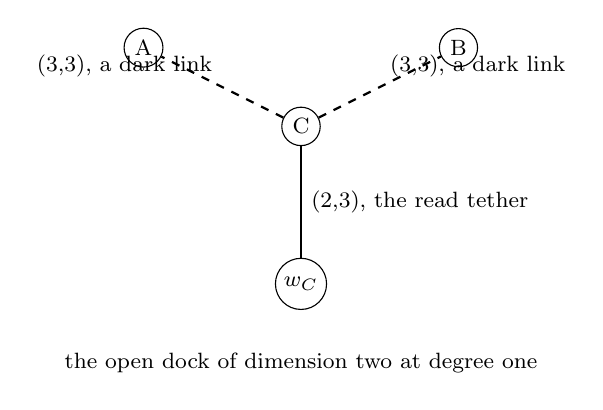
\begin{tikzpicture}[every node/.style={font=\footnotesize}]
\node[circle,draw,inner sep=2pt] (C) at (0,0) {C};
\node[circle,draw,inner sep=2pt] (A) at (-2,1) {A};
\node[circle,draw,inner sep=2pt] (B) at (2,1) {B};
\node[circle,draw,inner sep=2pt] (w) at (0,-2) {$w_C$};
\draw[dashed,thick] (C) -- node[above left] {(3,3), a dark link} (A);
\draw[dashed,thick] (C) -- node[above right] {(3,3), a dark link} (B);
\draw[thick] (C) -- node[right] {(2,3), the read tether} (w);
\node at (0,-3) {the open dock of dimension two at degree one};
\end{tikzpicture}
\caption{The closure site C of the universe web, of dimension three at degree three. Its two (3,3) links to the core sites A and B are the dark links, whose boundary count is the far-end dimension three at every rung, and its (2,3) link to the open dock $w_C$ is the read tether. With the fixed and moving interfaces these are the five elements of the balance.}
\end{figure}
\section{The universality of the move set}\label{mod:X-2-D538680-nmsu-t1}
\begin{chconditional}[The universality of the move set]\label{box:X-2-D538680-nmsu-t1:1}
Conditional on the results this entry rests on, each at its own standing. A move of the theory lies outside the Clifford group: the fourth-root phase generator of the re-matching carries the Weyl letter of the qutrit end to a monomial matrix whose phases are no clock pattern at the cube root of the end and so stands outside the Clifford group of the qutrit end, the same generator and the first transposition stand outside at the ququart end, and every other move stands inside at every end and genre. The groups the unitary one-end moves generate are finite at every end, equal to the Clifford group of the qubit end modulo scalars and parting from it at the qutrit and ququart ends, so the universality of the move set is read with the Clifford group adjoined by name under the Clifford-plus-non-Clifford theorem of the literature, the moves alone generating no dense group at any end.
\end{chconditional}
\chstanding{conditional theorem}
\chdeps{Definitions 1.1 to 1.6, Open result 92.1 and Theorem 92.2 and Open result 231.1}{no theorem beyond it at this release}
Every move is typed against the Clifford group at every end and genre by its action on the Weyl letters, the groups generated by the one-end moves are computed with their orders, and the universality is read with the adjoined group named. The algorithm entries are typed expressible at the first reading and gloss at the second, both readings given and neither adopted. What stands open is the universality of the gate set with the Clifford group adjoined by name and not by a move of the theory. The closure as the computation and the Hadamard as the coherent read stand at their own chapters.
\begin{chbridge}
The Clifford group of a register is the normalizer of its Pauli group, generated by the Hadamard, the phase and the controlled-not gates, and a circuit of Clifford gates alone is simulable classically by the stabilizer formalism. The correspondence is by name.
\end{chbridge}
\begin{chproof}[finite computation]
\textit{The premises.} The axiom and the six definitions of Section~\ref{mod:FRAMEWORK}, definitions. The moves of Section~\ref{mod:I-4-moves-in-one-table}, definitions. The moves as a gate set and the Weyl criterion of Section~\ref{mod:XIII-2-moves-as-a-gate-set-and-the-weyl-criterion}, a theorem. The field equation at the counting face of Section~\ref{mod:X-2-field-equation-at-the-counting-face}, an open result. The step transport, the holonomies, the pairing, the wash, the junction move, the dock move, the Hadamard read and the re-matching, at their own standings. The chain from the axiom to this result is seven chapters deep.

\textit{The procedure.} The input objects are the moves built as exact matrices or channels at the three ends (the qubit, the qutrit and the ququart) and the six genres, forty in all. They are the step transport as the permutation of the link register, the twenty-four holonomies, the pairing as the Bell unitary, the wash as the channel of the cap projectors, the junction move at its holonomy, the dock move at its step, the Hadamard read and the three generators of the re-matching (the first transposition, the full cycle and the fourth-root phase at the first direction). The test applied to each move at each end is the Clifford test. The Weyl letters $X$ (the shift) and $Z$ (the clock at the root of the end), with $ZX=\omega XZ$, are conjugated by the move, and the move is inside the Clifford group when every letter is carried to a Weyl letter at a phase and outside otherwise. The smallest instance is the Hadamard read at the qubit end. It carries $X$ to $Z$ and $Z$ to $X$ at the phase one, inside, and is of order two.

\textit{The totals.} The move is inside at every holonomy (the qubit holonomy carrying $X$ to $z^{12}X$ and $Z$ to itself, the three qutrit holonomies carrying every letter to a Weyl letter at a cube-root or half-turn phase), at the junction holonomy, where it is the identity at 120 of 120 loops, at every dock step, where it is a scalar at 10 of 10 readings, at the Bell unitary and at the re-matching transposition and cycle at the qubit and qutrit ends. It is outside at the fourth-root phase at the qutrit end, which carries $X$ to the monomial matrix
\begin{equation}
\begin{pmatrix}0&0&z^{6}\\ z^{18}&0&0\\ 0&z^{0}&0\end{pmatrix},\qquad z=e^{2\pi i/24},
\end{equation}
a shift of $X$ whose phases are no clock pattern at the cube root of the end, and at the ququart end likewise, with the transposition outside at the ququart end too, 3 of 40 tests outside in all, which is the statement. The groups generated by the unitary one-end moves are finite at every end, of orders $576$ at the qubit end (projective 24, equal to the Clifford group modulo scalars), $10\,368$ at the qutrit end and $6144$ at the ququart end, the latter two parting from the Clifford groups of projective orders $216$ and $768$ at a missing Fourier generator, so the moves alone generate no dense group at any end and the universality is read with the Clifford group adjoined by name.

\textit{The check.} Replacing the fourth-root phase by the identity, reading the step at the fixed near-major register and dropping the Hadamard read each move the inside and outside counts they name. Striking the text moves every cell. The result was reproduced by an independent route, two engines of different construction agreeing at every cell at both runs, with the cycle types of the step transport at 7 of 7, the traces of the holonomies at 24 of 24 and the re-matching orders $32$, $384$ and $6144$ as the controls.
\chcert{120}
\end{chproof}
\section{The universality of the (2,2) increment}\label{mod:X-2-D542409-w-unmi}
\begin{chwall}[The universality of the (2,2) increment]\label{box:X-2-D542409-w-unmi:1}
Face A, the increment per serial (2,2) insertion one cell at every admitted link and step with the (2,2) genre admitted at every web and no second genre admitted at every web, reads no at the universality clause. Face B reads yes with the first parting named: the metric increment per serial (2,2) insertion is one cell 96 at every one of the 1403 links with a qubit end across 77 of the 82 webs of the settled census at every step of the serial run, regardless of the content of the chain, the genre of the entered link, the far dimension, the body or the word, a theorem of the additive metric over the whole census; the serial (2,2) insertion is refused at the five webs with no qubit site, the gluon word of four qutrits, the Higgs word of two ququarts, the Higgs word, the leg piece and the free (3,4) genre of the Higgs-and-carrier entry, so (2,2) is admitted at 77 of 82 webs and no genre of the six is admitted at every web at the reading adopted; the first parting is the gluon word admitting no serial (2,2) insertion; at the readings beside the (3,4) genre attaches at every web under the inserted link alone naming the genre, and every genre at every link under a pair of qubits inserted anywhere, with the increment parting by the ends.
\end{chwall}
\chstanding{open result}
\chdeps{Definitions 1.1 to 1.6, Theorems 9.1 to 9.7 and Open result 9.8, Open result 92.1 and Theorem 92.2 and Theorem 195.1}{no theorem beyond it at this release}
The rule of the metric open result, a qubit site inserted at the entered qubit end with the far link keeping its genre, is applied at every link with a qubit end of the 82 webs of the settled census, and the increment of the register is read at every step; it is one element wherever the insertion is admitted, so the content independence half of the item is a theorem, while the admission itself fails at the five webs that carry no qubit. The field equation at the counting face stands at its own chapter.
\begin{chbridge}
The equivalence principle of the literature states that gravity couples to every form of energy with one and the same constant regardless of its composition, and in a gauge theory the coupling of the carrier is universal across the species it couples to \cite{Einstein1907,Will2014}. The correspondence is by name.
\end{chbridge}
\begin{chproof}[exhaustive census]
\textit{The premises.} The axiom and the six definitions of Section~\ref{mod:FRAMEWORK}, definitions. The link and its six genres of Section~\ref{mod:I-2-link-and-its-six-genres}, definitions. The body-alone office rule of Section~\ref{mod:VIII-2-body-alone-office-rule}, a theorem. The field equation at the counting face of Section~\ref{mod:X-2-field-equation-at-the-counting-face}, an open result. The chain from the axiom to this result is four chapters deep.

\textit{The census.} The set counted is the 82 webs of the settled census, the sixty-four webs of the web table in their order, the proton, the neutron, the deuteron, the one-link web and the two stars of the body-alone entry, the universe web at 444 sites and 551 links, the tau sink at 16 sites and the ten bodies and words of the Higgs-and-carrier entry, 1912 sites and 2381 links with 356 (2,2) links, 255 of the table and 85 of the universe web. The property tested at every link with a qubit end is the increment of the register under the serial insertion, a qubit site inserted at the entered qubit end with the far link keeping its genre, at the steps k 1, 2 and 3; the register is the sum of the caps and the cap of a genre its Born count. The increment reads 96 at every one of 1403 admitted links of 77 webs at every step, the cap of the (2,2) genre,
\begin{equation}
96 = 24 + 18\cdot 2 + 12\cdot 2 + 3\cdot 4,
\end{equation}
the distinct increments one and the first parting none, at a (2,3) link with the far end a qutrit and at a (2,4) link with the far end a ququart alike, since the inserted link is a (2,2) link and the far link keeps its genre; the chains of the metric open result re-meet at 96 at every step, the 1643 uniform chains of the table partition its links by genre, 231, 45, 651, 488, 217 and 11, of which 927 admit the insertion, and the junction stars number 577 with 255 admitting. The webs admitting no link are the five with no qubit site. Over the six genres at the reading adopted the (2,2) genre is admitted at 77 of 82 webs, the (3,3) at 78 with the Higgs word of two ququarts first missing, the (4,4) at 75 with the one-link web first missing, and the three unequal genres at 0 of 82 since the far link cannot keep its genre at an off-diagonal insertion; the second universal genre is none. The smallest case is the electron web at its hub-unit pair, the register 8613 at k 0 and 8709 at k 1, the increment 96, checked by hand from the caps. So face A reads no at the universality clause and face B reads yes with the first parting the gluon word, a parting of the admission clause and of neither form the item words, a typing left to the return. The result is certified at the repository.

\textit{The check.} The electron web struck from the census moves the web count to 81 with the increment unmoved, the inserted sites read as qutrits move the increment to 542, 1036 and 1466 by the far dimension, every web doubled as a disjoint copy doubles the register while the increment stays 96, the genre-to-cap map transposed moves the one cell to 5100, and the text struck excludes the run, 5 of 5 as pinned. The controls read the same at 13 of 13, among them the metric open result re-met at 9 of 9 chains, the caps equal to the Born counts at six genres and the register of the universe web $513\,055$ equal to the sum of the caps over its 551 links. The result was reproduced by an independent route, two engines of different construction agreeing at every cell at both runs.
\chcert{1403}
\end{chproof}
\section{The linear field equation at the counting face}\label{mod:X-2-D543262-w-lnfe}
\begin{chwall}[The linear field equation at the counting face]\label{box:X-2-D543262-w-lnfe:1}
Face A, the washed Laplacian of the (2,2) count equal to the office density at the counting face multiplied by the (2,2) coupling at every settled web, with the non-pair Laplacian the source, reads no at 0 of 21 webs. Face B reads yes with the first parting named: at the 21 rung-reading webs of the ladder of the curvature chapter the washed Laplacian of the (2,2) count and the coupling of the two-point function multiplied by the washed non-pair Laplacian are equal at 0 of 21 webs and at 0 of 1546 cells of the universe web, the first parting at the closure-site body at rung 0 at its first site B31.A, a site of dimension 3 with three links and no (2,2) link, at the diagonal cell reading 0 at the left side against $5/128 + (5/128)\sqrt{2}$ at the right, the coupling $5/384 + (5/384)\sqrt{2}$ multiplied by the source cell 3, and at the universe web at the hub B00.F reading 0 against $5/96 + (5/96)\sqrt{2}$; the two sides part by construction at every cell where a link is not of the pair genre, a rational left cell against a right cell with a nonzero root-two coordinate, and at every cell of a pair link, a nonzero left cell against a zero source cell, so the equation holds at no settled web but one with no links at all; the coupling between the two sides as the trace ratio is an exact rational at every web, 85 over 466 at the universe web and 1 over 4 at the closure-site body, equal to the two-point element at 0 of 21; the source against the office density is equal at 0 of 444 sites of the universe web, B00.F reading 4 against 36.
\end{chwall}
\chstanding{open result}
\chdeps{Definitions 1.1 to 1.6, Theorems 78.1 to 78.3, Theorems 90.1 to 90.4 and Open result 92.1 and Theorem 92.2}{no theorem beyond it at this release}
The washed Laplacian of the (2,2) count is built and washed at every web of the ladder, the source is built as the washed Laplacian of the links not of the pair genre and compared with the office density at every site, the coupling is printed at every web as the trace ratio and against the two-point element, and the two sides of the linear equation are compared cell by cell. The two sides live on disjoint links and in different rings, so the equation names an open result at its first site. The curvature and the field equation stand at their own chapters.
\begin{chbridge}
The linearized field equation of gravitation in the literature sets the Laplacian of the metric perturbation proportional to the energy density of its source with the gravitational constant as the coupling, and in electrodynamics the Laplacian of the potential is proportional to the charge density with the fine-structure constant setting the strength \cite{Einstein1916,Peskin1995}. The correspondence is by name.
\end{chbridge}
\begin{chproof}[exhaustive census with its exact part]
\textit{The premises.} The axiom and the six definitions of Section~\ref{mod:FRAMEWORK}, definitions. The curvature as the graph Laplacian washed over the ladder of Section~\ref{mod:X-1-curvature-as-the-graph-laplacian-washed-over-the-ladder}, a theorem. The field equation at the counting face of Section~\ref{mod:X-2-field-equation-at-the-counting-face}, an open result. The Ward identity and the anomaly sums of Section~\ref{mod:IV-8-ward-identity-and-the-anomaly-sums}, a theorem. The chain from the axiom to this result is five chapters deep.

\textit{The census.} The set counted is the 21 rung-reading webs of the ladder of the curvature chapter at the three readings and rungs 0 to 6, rebuilt from the closure entries at 21 of 21 webs and 105 of 105 ladder cells. At every web the left side is the washed Laplacian of the (2,2) count, symmetric with the row sums zero at 21 of 21, the trace 170 at the universe web and 6 at the closure-site body; the source is the washed Laplacian of the links not of the pair genre, the trace 932 at the universe web and 24 at the closure-site body, the sum of the two sides equal to the washed Laplacian at every cell of 21 of 21 webs; the office density at the reading adopted is the first-power flux at a site, 8836 over the universe web; the coupling is read by key at the dressing table of the two-point entry, $(30 + 30\sqrt{2})/2304 = 5/384 + (5/384)\sqrt{2}$. The property tested at every cell is the equality of the left cell with the coupling multiplied by the source cell: at the universe web 0 of 1546 cells and at the closure-site body 0 of 42, the first parting at the first web of the frozen order, the closure-site body at rung 0 at its first site B31.A, the left cell 0 against $(5/384 + (5/384)\sqrt{2})\cdot 3 = 5/128 + (5/128)\sqrt{2}$, the smallest case worked at the figure. The coupling between the two sides as the trace ratio reads 85 over 466 at the universe web and 1 over 4 at the closure-site body, an exact rational at 21 of 21 webs and equal to the two-point element at 0 of 21; the source against the office density is equal at 0 of 444 sites. So the rule pinned ahead reads face A no and face B yes. The result is certified at the repository.

\textit{The check.} The source struck, the (2,3) Laplacian in place of the (2,2), the coupling struck to one, the text struck and the pair ket at the join appended as a twenty-second web each move the cells they name, 5 of 5 as pinned. The controls read the same at 14 of 15 at the pinned engines and at 15 of 15 at the return route, the one spelling of the serial increment keys re-keyed as sparse maps. The result was reproduced by an independent route, two engines of different construction agreeing at every cell at both runs.
\chcert{1546}
\end{chproof}
\begin{figure}[h]
\centering
\begin{adjustbox}{max width=\linewidth}\begin{tabular}{lll}
\hline
site & the left cell & the coupling multiplied by the source cell \\
\hline
B31.A & 0 & $(5/384 + (5/384)\sqrt{2})\cdot 3 = 5/128 + (5/128)\sqrt{2}$ \\
\hline
\end{tabular}\end{adjustbox}
\caption{The smallest case, the closure-site body at rung 0 at its first site B31.A: the left cell 0 against the coupling multiplied by the source cell 3, a rational against an element with a nonzero root-two coordinate.}
\end{figure}
\section{The nonlinear field equation at the counting face}\label{mod:X-2-D543652-w-nlfe}
\begin{chwall}[The nonlinear field equation at the counting face]\label{box:X-2-D543652-w-nlfe:1}
Face A, the nonlinear field equation closing at every settled web, the (2,2) count plus the vacuum term equal to the coupling of the two-point function multiplied by the office density plus the count itself, closing under the row-sum-zero operator with the density conserved along the chains and the vacuum term uniform, reads no at 0 of 21 webs. Face B reads yes with the first parting named: at the 21 rung-reading webs of the ladder of the curvature chapter the equation closes at 0 of 444 sites of the universe web and at no site of any web, the first parting at the closure-site body at rung 0 at its first site B31.A under the readings closure and sources, the count 0 plus the vacuum term at the depth 3 of the site, $1/23\,328$, against the coupling multiplied by the density 30, $25/64 + (25/64)\sqrt{2}$, and the self-source 0 against the office density 30, at the universe web at B00.F $1/839\,808$ against $15/32 + (15/32)\sqrt{2}$; the two sources part by construction at every site with a link; the closure under the row-sum-zero operator reduces to the conservation of the density along the chains at every settled web, the operator applied to the count zero everywhere with every chain one link, and holds at 430 of 444 sites and 78 of 85 chains of the universe web and at every site and chain of the fourteen webs of the first two readings, the first unconserved chain from B07.w1 to B07.b3 at 4 against 12; the vacuum term at the depth of the site is uniform at 0 of 21 webs, 14 distinct values at the universe web, with the term $1/1\,088\,391\,168$ at the depth exponent 6 re-met by key.
\end{chwall}
\chstanding{open result}
\chdeps{Definitions 1.1 to 1.6, Theorems 90.1 to 90.4, Open result 92.1 and Theorem 92.2 and Theorem 115.1}{no theorem beyond it at this release}
The two sources of the nonlinear equation, the count at a site and the office density, are built and compared at every site of every web of the ladder, the closure under the row-sum-zero operator and the conservation of the density along the chains are read at every site and chain, and the vacuum term is printed at every site at the depth read there. The count is not its own source beside the density at the coupling of the two-point function at any web, and the closure under the operator is the conservation of the density. The curvature and the field equation stand at their own chapters.
\begin{chbridge}
The field equations of gravitation are nonlinear, the geometry sourcing itself, their divergence vanishes by the Bianchi identity so that the source is conserved, and the cosmological constant enters as one term uniform over space \cite{Einstein1916,Einstein1917,Wald1984}. The correspondence is by name.
\end{chbridge}
\begin{chproof}[finite computation with its census and its exact part]
\textit{The premises.} The axiom and the six definitions of Section~\ref{mod:FRAMEWORK}, definitions. The curvature as the washed Laplacian of Section~\ref{mod:X-1-curvature-as-the-graph-laplacian-washed-over-the-ladder}, a theorem. The field equation at the counting face of Section~\ref{mod:X-2-field-equation-at-the-counting-face}, an open result. The cosmological term at the depth exponent of Section~\ref{mod:X-6-cosmological-term-at-the-depth-exponent}, a theorem. The chain from the axiom to this result is five chapters deep.

\textit{The procedure.} At every one of the 21 webs of the ladder the row-sum-zero operator is the washed Laplacian of the (2,2) links with the count on its diagonal, symmetric with the row and column sums zero, the count sum 170 at the universe web and 1 at each of the six qubit legs of the closure-site body; the self-source is the count at the site; the office density is the first-power flux at the site, the sum over its links of the product of the end dimensions; the vacuum term at a site is the closure constant 2 over the whole register 36 to the depth read at the site, the depth its eccentricity by breadth-first passage count over the links of its component. The equation of the item at a site reads the count plus the vacuum term against the coupling of the two-point function multiplied by the density plus the count; the closure reading applies the operator to both sides, under which the vacuum term drops by the row sums zero; the conservation reading asks the density to be one value along every chain, the chains the components of the pair links.

\textit{The totals.} The two sources are equal at 0 of 444 sites of the universe web, the first parting B00.F at the count 0 against the density 36, and at 0 of 12 sites of the closure-site body, B31.A at 0 against 30, since a link adds one to the count of each end and the product of the end dimensions, at least four, to the density of each end. From the coupling and the density at B31.A, by the product, we obtain the right side
\begin{equation}
\Bigl(\frac{5}{384} + \frac{5}{384}\sqrt{2}\Bigr)\cdot 30 + 0 = \frac{25}{64} + \frac{25}{64}\sqrt{2}
\end{equation}
against the left side $0 + 2/36^{3} = 1/23\,328$ at the depth 3, the smallest case worked on the page, and at B00.F the left side $2/36^{4} = 1/839\,808$ against $15/32 + (15/32)\sqrt{2}$; a rational stands against an element with a nonzero root-two coordinate at every site unless the density and the count are both zero, so the equation closes at 0 of 21 webs. The operator applied to the count is zero at every site of every web, every chain being one link with the count 1 at both ends, so the closure under the operator reads the operator applied to the density alone, equal at 430 of 444 sites of the universe web with the first parting B07.b3 at 0 against $5/48 + (5/48)\sqrt{2}$, at 12 of 12 sites of the closure-site body at every rung of the first two readings and at every site of 14 of 21 webs; the density is one value along 78 of 85 chains of the universe web, the first unconserved from B07.w1 to B07.b3 at 4 against 12, along the three chains of the closure-site body at 12 and 12, and along every chain of 14 of 21 webs, the closure-parting sites equal to the unconserved sites at 21 of 21 webs. The depth census of the universe web reads 1, 8, 18, 48, 72, 92, 80, 38, 44, 10, 18, 4, 7, 4 at the depths 1 to 14 with 14 distinct term values, the first parting B00.G at the depth 3 against B00.F at the depth 4, and at the closure-site body three distinct values with the first parting at the hub B31.H1 at the depth 4 against 3, uniform at 0 of 21 webs; the term at the depth exponent 6, $1/1\,088\,391\,168$, is one value at every site by construction and equals the term of the curvature-coefficient open result and the counting-face open result by key. The first order beside, the diagonal reading of the linear equation, parts at B31.A and B00.F at the cells of that open result, re-met by key at 25 of 25. So the rule pinned ahead reads face A no and face B yes with the first parting named.

\textit{The check.} The self-source struck moves the self-source sum from 170 to 0, the (2,3) count in place of the (2,2) moves the count sum to 68, the vacuum term struck moves the left cell to 0 with the vacuum reading uniform by the strike, the text struck excludes the run, and the pair ket appended as a twenty-second web moves the compared webs to 22 of 22, 5 of 5 as pinned. The controls read the same at 17 of 17, among them the linear equation re-met at its coupling at 25 of 25 keys and the curvature-coefficient open result at 30 of 30 cells. The result was reproduced by an independent route, two engines of different construction agreeing at every cell at both runs.
\chcert{444}
\end{chproof}
\begin{figure}[h]
\centering
\begin{adjustbox}{max width=\linewidth}\begin{tabular}{lll}
\hline
site & the left side & the right side \\
\hline
B31.A at the depth 3 & $2/36^{3} = 1/23\,328$ & $25/64 + (25/64)\sqrt{2}$ \\
B00.F at the depth 4 & $2/36^{4} = 1/839\,808$ & $15/32 + (15/32)\sqrt{2}$ \\
\hline
\end{tabular}\end{adjustbox}
\caption{The smallest case, the site B31.A at the depth 3, with the hub B00.F beside: a rational on the left against an element with a nonzero root-two coordinate on the right, so the equation closes at 0 of 21 webs.}
\end{figure}
\section{The field equation as the first law}\label{mod:X-2-D543764-w-flfw}
\begin{chwall}[The field equation as the first law]\label{box:X-2-D543764-w-flfw:1}
Face A, the count of records crossing the horizon at one depth step one proportion of the office flux across it at every step with the coupling of the two-point function its constant, reads no. Face B reads yes with the first parting named: at the horizon web the records newly hidden at the six depth steps read 0, 3, 0, 3, 0, 3 at the open-end face and 0, 3, 3, 3, 3, 3 at the docking order, while the first-power flux through the fixed cut is 24 at every rung, the two (3,3) wires at 9 each and the (2,3) tether at 6, and through the moving cut 24 then 12 at every rung of the open-end face and 24, 12, 30, 14, 14, 18, 24 at the docking order, so the ratio of the crossing count to the flux reads 0 at the first step of every series and 1 over 8 at the second step at the fixed cut, parting at step 2 at 4 of 4 series; against the coupling $5/384 + (5/384)\sqrt{2}$ the ratio, a rational at every step, parts at 24 of 24 steps, the first parting at the open-end face at the fixed interface at step 1, 0 against the coupling; against the area-law coefficient at the count reading, 1 over 4, 1 over 4, 1 over 2, 1 over 2, 3 over 4, 3 over 4 and 1 across the rungs of the fixed cut, the ratio parts at 24 of 24 steps; the counting-face equation of the linear open result re-derived at the ratio holds at 0 of 18 settled webs with a step.
\end{chwall}
\chstanding{open result}
\chdeps{Definitions 1.1 to 1.6, Open result 92.1 and Theorem 92.2 and Theorems 99.1 and 99.2, Open results 99.3 and 99.4, Theorem 99.5 and Open result 99.6}{no theorem beyond it at this release}
The records newly hidden at each depth step of the horizon web are counted from the hidden records of the area-law open result, the first-power flux through the crossing links is summed at every cut and rung, and their ratio is compared with the coupling of the two-point function and with the area-law coefficient at every step, the linear equation then re-derived with that ratio in place of the coupling. No record crosses at the first step while the flux is 24, so the ratio is zero where the coupling is not, and three records cross at the second step, so it is no constant of the web. The field equation, the horizon and the area law stand at their own chapters.
\begin{chbridge}
The first law of horizon thermodynamics in the literature relates the entropy change of a horizon to the energy flux across it in one proportion whose constant is the temperature, and the field equation itself follows from that law applied at every point \cite{Bekenstein1973,Jacobson1995}. The correspondence is by name.
\end{chbridge}
\begin{chproof}[exhaustive census]
\textit{The premises.} The axiom and the six definitions of Section~\ref{mod:FRAMEWORK}, definitions. The field equation at the counting face of Section~\ref{mod:X-2-field-equation-at-the-counting-face}, an open result. The horizon at every rung of Section~\ref{mod:X-3-horizon-at-every-rung-and-the-horizon-web-as-a-seeded-saturation}, a theorem. The area law at the cut of the chapter titled The area law at the cut (chapter~\ref{mod:X-2a-D542325-w-arlw}), an open result. The chain from the axiom to this result is five chapters deep.

\textit{The census.} The set counted is the depth steps of the horizon web at the two admitted readings of the attachment site, the open-end face and the docking order, at the fixed and the moving cut, 24 step cells of the four series, with the closure-site face beside at rung 0 alone. The hidden records are read from the area-law open result by locator, 3, 3, 6, 6, 9, 9, 12 at the open-end face and 3, 3, 6, 9, 12, 15, 18 at the docking order, equal to the closure table of the horizon chapter; the records newly hidden at a step are the hidden count at the rung less the count at the rung beneath, 0, 3, 0, 3, 0, 3 and 0, 3, 3, 3, 3, 3 across the steps 1 to 6, exact at 36 of 36 step cells over the readings. The crossing links of the area-law open result are parsed into their end dimensions and the act of a link read as the product of its end dimensions, the first-power rule of the counting-face chapter, so the flux through the fixed cut is
\begin{equation}
9 + 9 + 6 = 24
\end{equation}
at every rung, the two (3,3) wires and the (2,3) tether, and through the moving cut 24, 12, 12, 12, 12, 12, 12 at the open-end face and 24, 12, 30, 14, 14, 18, 24 at the docking order, every flux a nonzero integer at 42 of 42 cuts, equal to the flux cells of the counting-face chapter at every element and rung. The ratio of the crossing count to the flux at the lower rung of the pair reads 0, 1 over 8, 0, 1 over 8, 0, 1 over 8 at the open-end face at the fixed cut, 0, 1 over 4, 0, 1 over 4, 0, 1 over 4 at its moving cut, 0 then 1 over 8 at every step at the docking order at the fixed cut and 0, 1 over 4, 1 over 10, 3 over 14, 3 over 14, 1 over 6 at its moving cut, parting at step 2 at 4 of 4 series, the smallest case the first two steps at the fixed cut, 0 over 24 then 3 over 24. Against the coupling $5/384 + (5/384)\sqrt{2}$ the ratio differs at 24 of 24 steps, the difference at the first step minus the coupling and at the second step $43/384 - (5/384)\sqrt{2}$; against the area-law coefficient at the count reading, 1 over 4, 1 over 4, 1 over 2, 1 over 2, 3 over 4, 3 over 4, 1 at the fixed cut, it differs at 24 of 24; the linear equation re-derived with the ratio at the fixed cut in place of the coupling holds at 0 of 18 webs with a step, the first parting at the closure-site body at rung 1 at its first pair site B31.q1 reading 1 against 0, and the linear open result itself is re-met at its own coupling at every web with its first parting cell string for string. So the rule pinned ahead reads face A no and face B yes with the first parting the coupling at the open-end face at the fixed interface at step 1, the proportionality itself parting one step on.

\textit{The check.} The hidden records at rung 2 struck move the step count to minus 3, the (2,3) flux in place of the office flux moves the flux to 6 with every ratio, the coupling struck to one moves every difference, a horizon with no hidden record moves the series letter to constant at every step, and the text struck excludes the run, 5 of 5 as pinned. The controls read the same at 13 of 13. The result was reproduced by an independent route, two engines of different construction agreeing at every cell at both runs.
\chcert{24}
\end{chproof}
\par\medskip\noindent{\itshape The next chapter reads the horizon at every rung.}\label{narr:close:10-2}\par
\section{The area law at the horizon web}\label{mod:X-2a-D542325-w-arlw}
\chdesig{6-2a}{10-2a}{X-2a-D542325-w-arlw}{X-2a-D542325-w-arlw}
\begin{chwall}[The area law at the horizon web]\label{box:X-2a-D542325-w-arlw:1}
Face A, the hidden records proportional to the counted (2,2) crossings at every rung with the constant printed as an exact element, reads no. Face B reads yes with the first parting named: at the horizon web, the universe web of the hand-off at 444 sites and 551 links with its rungs 0 to 6 as the closure table of the horizon chapter specifies them at the open-end face and the docking-order face, the cut at the slot B31.C severs two (3,3) wires and the (2,3) tether at every rung and the cut at the newest rung severs (2,3), (2,4) and (3,4) links alone, the counted (2,2) crossings 0 at 7 of 7 rungs at every reading and interface, so the area at the (2,2) face reads 0 at every rung while the hidden records read 3, 3, 6, 6, 9, 9, 12 at the open-end face and 3, 3, 6, 9, 12, 15, 18 at the docking order, the ratio of the hidden records to the counted crossings undefined at every rung of the four series, the first parting at the open-end face at the fixed interface at rung 0, the hidden records 3 against the counted crossings 0; the series beside part too, the hidden records over every crossing link 1, 1, 2, 2, 3, 3, 4 at the fixed interface of the open-end face parting at rung 2, and over the summed caps 2391 at the fixed interface parting alike.
\end{chwall}
\chstanding{open result}
\chdeps{Definitions 1.1 to 1.6, Theorems 99.1 and 99.2, Open results 99.3 and 99.4, Theorem 99.5 and Open result 99.6 and Theorems 113.1 and 113.2}{no theorem beyond it at this release}
The cut of the horizon web is censused by genre at every rung at two admitted readings of the attachment site and at the fixed and the moving interface, the area read as the counted (2,2) crossings at the increment of the metric open result with the summed caps, the ticks and the tower beside, and the hidden records counted as the records of the closure at the qubit ends. The (2,2) links sit inside the bodies and never at the cut, so no constant of proportion exists at any rung and the area law at the (2,2) face is an open result at rung 0. The horizon at every rung and the register tower stand at their own chapters.
\begin{chbridge}
The entropy of a black hole in the literature is proportional to the area of its horizon, one quarter of the area in Planck units, and the holographic principle bounds the degrees of freedom of a region by the area of its boundary \cite{Bekenstein1973,Hawking1975,Bousso2002}. The correspondence is by name.
\end{chbridge}
\begin{chproof}[finite computation with its census and its exact part]
\textit{The premises.} The axiom and the six definitions of Section~\ref{mod:FRAMEWORK}, definitions. The horizon at every rung of Section~\ref{mod:X-3-horizon-at-every-rung-and-the-horizon-web-as-a-seeded-saturation}, a theorem. The area law at the cut of the chapter titled The area law at the cut (chapter~\ref{mod:X-2a-D542325-w-arlw}), at its standing. The register tower of Section~\ref{mod:X-5-register-tower-and-the-metric}, a theorem. The chain from the axiom to this result is five chapters deep.

\textit{The procedure.} The universe web of the hand-off is parsed whole at 444 sites, 551 links, 27 components and the genres 85, 34, 229, 134, 67 and 2 at (2,2) to (4,4) with 54 sites of degree one, the open dock B31.wC of dimension 2, the tether C to wC a (2,3) link, the slot B31.C of dimension 3 at degree 3 and the star severed by the cut, A to C and B to C at (3,3) and C to wC at (2,3). The rungs 0 to 6 are read at the open-end face, the chain of alternating dimensions joined by (2,3) links, and at the docking order, the six leaves docked at the named sites, the closure-site face refused beyond rung 0 as the closure table prints it. At the fixed interface, the cut at the slot, and at the moving interface, the cut at the attachment site of the newest rung, the crossing links are censused by genre and the (2,2) crossings counted; the area is the counted crossings multiplied by the increment 96 of the metric open result, the summed area every crossing link at its cap, and the hidden records are counted as 3 per qubit end behind the cut and 0 per qutrit end under the sign clause.

\textit{The totals.} At the fixed interface the census reads 0, 1, 0, 2, 0, 0 at the six genres at every rung and reading, the counted (2,2) crossings 0, the total 3 and the horizon counts 9 at both alphabets; at the moving interface the open-end face severs the two (2,3) links from rung 1 and the docking order severs (2,3), (2,4) and (3,4) links alone, the totals 3, 2, 3, 2, 2, 2, 3, so the counted (2,2) crossings read 0 at 28 of 28 cells. The counted area is 0 at every rung, the summed area at the fixed interface
\begin{equation}
1036 + 1036 + 319 = 2391
\end{equation}
at every rung, 638 at the moving interface of the open-end face from rung 1 and 2391, 638, 4425, 1225, 1225, 2372, 2691 at the docking order, with the ticks 3 at the fixed interface and the tower of the depth-scale chapter beside, 24 multiplied by 36 to the rung, equal at 7 of 7 rungs to the horizon chapter, the cap-wave census and the depth-scale tower. The qubit ends behind the cut read 1, 1, 2, 2, 3, 3, 4 at the open-end face and 1, 1, 2, 3, 4, 5, 6 at the docking order, so the hidden records read 3, 3, 6, 6, 9, 9, 12 and 3, 3, 6, 9, 12, 15, 18, equal to the closure table at 15 of 15 cells; the smallest instance is rung 0, one qubit end behind the fixed cut and 3 hidden records against 0 counted crossings. The ratio of the hidden records to the counted crossings is undefined at every one of the 28 cells of the four series, so face A reads no and face B reads yes at the open-end face at the fixed interface at rung 0; beside, the ratio over every crossing link reads 1, 1, 2, 2, 3, 3, 4 at the fixed interface and parts at rung 2, and the ratio over the summed caps reads 1 over 797 at rung 0 and parts at rung 2 at the fixed interface and at rung 1 at the moving interfaces, every ratio an exact rational or undefined. The result is certified at the repository.

\textit{The check.} The rung 3 struck moves the hidden records at the docking order from 9 to 6, the (2,3) crossings in place of the (2,2) moves the counted crossings to 1 with the ratios then defined and parting, the horizon shifted to B31.A moves the census to two (3,3) wires and a (3,4) link, the unwashed count at the Weyl letters moves the hidden records from 3 to 11, and the text struck excludes the run, 5 of 5 as pinned. The controls read the same at 12 of 12, among them the closure table at 21 of 21, the horizon table at 12 of 12 and the cap-wave census at 10 of 10. The result was reproduced by an independent route, two engines of different construction agreeing at every cell at both runs.
\chcert{300}
\end{chproof}
\begin{figure}[htbp]\centering
\setlength{\unitlength}{1mm}
\begin{picture}(160,36)(0,0)
\put(2,26){\framebox(8,6){\scriptsize 3}}
\put(2,4){\framebox(8,6){\scriptsize 3}}
\put(24,15){\framebox(8,6){\scriptsize 3}}
\put(20,11){\makebox(16,3){\tiny B31.C}}
\put(50,15){\framebox(8,6){\scriptsize 2}}
\put(46,11){\makebox(16,3){\tiny B31.wC}}
\qbezier(10,29)(17,25)(24,21)
\qbezier(10,7)(17,11)(24,15)
\qbezier(32,18)(41,18)(50,18)
\put(20,8){\dashbox{1}(17,20){}}
\put(14,30){\makebox(28,3){\tiny the fixed cut}}
\put(8,26){\makebox(16,3){\tiny (3,3) cap 1036}}
\put(8,8){\makebox(16,3){\tiny (3,3) cap 1036}}
\put(33,19){\makebox(16,3){\tiny (2,3) cap 319}}
\put(62,28){\makebox(98,3){\scriptsize the links crossing the cut: A-C:(3,3); B-C:(3,3); C-wC:(2,3); the wholes 81, 81 and 36, the cut register 236196}}
\put(62,22){\makebox(98,3){\scriptsize the increment 96 per serial (2,2) link; the caps by genre 22:96, 23:319, 24:906, 33:1036, 34:2053, 44:5100}}
\put(62,16){\makebox(98,3){\scriptsize the formal log of the cut register $2\log 2+10\log 3$; the dark register 6561 (the two (3,3) wires)}}
\put(62,10){\makebox(98,3){\scriptsize the universe web of record at 444 sites and 551 links; the counted (2,2) crossings 0 at every rung}}
\end{picture}
\par\smallskip
{\scriptsize\setlength{\tabcolsep}{3pt}\begin{adjustbox}{max width=\linewidth}\begin{tabular}{lrrrrrrr}
rung & 0 & 1 & 2 & 3 & 4 & 5 & 6 \\
\hline
\multicolumn{8}{l}{\textit{the fixed cut at both faces}} \\
links crossing the cut by genre & (2,3): 1, (3,3): 2 & (2,3): 1, (3,3): 2 & (2,3): 1, (3,3): 2 & (2,3): 1, (3,3): 2 & (2,3): 1, (3,3): 2 & (2,3): 1, (3,3): 2 & (2,3): 1, (3,3): 2 \\
counted (2,2) crossings & 0 & 0 & 0 & 0 & 0 & 0 & 0 \\
counted area & 0 & 0 & 0 & 0 & 0 & 0 & 0 \\
summed area over the caps & 2391 & 2391 & 2391 & 2391 & 2391 & 2391 & 2391 \\
ticks, one per crossing link & 3 & 3 & 3 & 3 & 3 & 3 & 3 \\
cut register & 236196 & 236196 & 236196 & 236196 & 236196 & 236196 & 236196 \\
(2,2) depth of the cut & 0 & 96 & 192 & 288 & 384 & 480 & 576 \\
\hline
\multicolumn{8}{l}{\textit{the open-end face}} \\
hidden records & 3 & 3 & 6 & 6 & 9 & 9 & 12 \\
records over the counted (2,2) crossings & undefined & undefined & undefined & undefined & undefined & undefined & undefined \\
records over every crossing link & 1 & 1 & 2 & 2 & 3 & 3 & 4 \\
records over the summed area & $1/797$ & $1/797$ & $2/797$ & $2/797$ & $3/797$ & $3/797$ & $4/797$ \\
records over the log of the cut register & $3/(2\log 2+10\log 3)$ & $3/(2\log 2+10\log 3)$ & $3/(1\log 2+5\log 3)$ & $3/(1\log 2+5\log 3)$ & $9/(2\log 2+10\log 3)$ & $9/(2\log 2+10\log 3)$ & $6/(1\log 2+5\log 3)$ \\
records over the (2,2) depth of the cut & undefined & $1/32$ & $1/32$ & $1/48$ & $3/128$ & $3/160$ & $1/48$ \\
register at the moving cut & 236196 & 1296 & 1296 & 1296 & 1296 & 1296 & 1296 \\
\hline
\multicolumn{8}{l}{\textit{the docking-lemma face}} \\
hidden records & 3 & 3 & 6 & 9 & 12 & 15 & 18 \\
records over the counted (2,2) crossings & undefined & undefined & undefined & undefined & undefined & undefined & undefined \\
records over every crossing link & 1 & 1 & 2 & 3 & 4 & 5 & 6 \\
records over the summed area & $1/797$ & $1/797$ & $2/797$ & $3/797$ & $4/797$ & $5/797$ & $6/797$ \\
records over the log of the cut register & $3/(2\log 2+10\log 3)$ & $3/(2\log 2+10\log 3)$ & $3/(1\log 2+5\log 3)$ & $9/(2\log 2+10\log 3)$ & $6/(1\log 2+5\log 3)$ & $15/(2\log 2+10\log 3)$ & $9/(1\log 2+5\log 3)$ \\
records over the (2,2) depth of the cut & undefined & $1/32$ & $1/32$ & $1/32$ & $1/32$ & $1/32$ & $1/32$ \\
register at the moving cut & 236196 & 1296 & 746496 & 2304 & 2304 & 5184 & 186624 \\
\hline
\end{tabular}\end{adjustbox}}
\caption{The area law per rung at the fixed cut of the horizon web of record: the links crossing the cut by genre, the counted (2,2) crossings, the counted and summed areas in the units of the increment and the caps, the hidden records at the two faces, the cut register with its formal log and the coefficient of the hidden records to the log at every rung 0 to 6 (the area law). No (2,2) link crosses the cut at any rung, so the ratio of the hidden records to the counted crossings is undefined at every rung, and the cut register is one register at every rung while the hidden records grow by three per qubit rung.}\label{fig:X-2a-542325-arealaw}
\end{figure}
\begin{figure}[h]
\centering
\begin{adjustbox}{max width=\linewidth}\begin{tabular}{lrrr}
\hline
rung at the open-end face & qubit ends behind the cut & hidden records & counted crossings \\
\hline
0 & 1 & 3 & 0 \\
6 & 4 & 12 & 0 \\
\hline
\end{tabular}\end{adjustbox}
\caption{The smallest instance at the fixed interface, rung 0: one qubit end behind the cut and 3 hidden records against 0 counted crossings, the ratio undefined, as at every one of the 28 cells; rung 6 beside.}
\end{figure}
\section*{The Horizon}
\addcontentsline{toc}{section}{The Horizon}
\section{The horizon at every rung and the horizon web as a seeded saturation}\label{mod:X-3-horizon-at-every-rung-and-the-horizon-web-as-a-seeded-saturation}
\chdesig{6-3}{10-3}{X-3-horizon-at-every-rung-and-the-horizon-web-as-a-seeded-saturation}{X-3-D543792-abrh-t1}
\label{narr:open:10-3}Theorem~99.1 reads the horizon at every rung as a seeded saturation, Theorem~99.2 the horizon register face at the closure, Theorem~99.5 the horizon web as a non-sink at the bound, and the open results beside them, Open result~99.3, Open result~99.4, Open result~99.6, Open result~100.1 and Open result~101.1, carry the horizon web to the cap.
\begin{chconditional}[The horizon at every rung as a seeded saturation]\label{box:X-3-horizon-at-every-rung-and-the-horizon-web-as-a-seeded-saturation:1}
Conditional on the results this entry rests on, each at its own standing. The iterated closure of the universe web under the rule of records, built at rungs zero to six at the three readings of the attachment site, carries the horizon count at the closure interface at every rung, the fixed interface at nine, the register fraction of every readout unchanged, and the point group of the one-rung web the dihedral group of order eight.
\end{chconditional}
\chstanding{conditional theorem}
\chdeps{Definitions 1.1 to 1.6, Open results 241.1 and 241.2, Theorems 241.3 and 241.4 and Open results 241.5 to 241.7 and Open results 245.1 and 245.2, Theorem 245.3, Open results 245.4 to 245.8 and Theorem 245.9}{the theorems of Chapters 6-2, 6-2a, 6-3 to 6-4, 6-6}
\begin{chconditional}[Horizon register face at the closure]\label{box:X-3-horizon-at-every-rung-and-the-horizon-web-as-a-seeded-saturation:2}
Conditional on depth scale at the register tower, horizon at every rung from iterated closure and boundary count at the counting face, each at its own standing. The gravitational coupling object and the expansion object meet at one face of the horizon register, the valence face at the rung count sixty-three, both read through the same closure interface with the register exponent equal to the closure count there, where the closure is saturated at its free-direction bound, while at the cap face the closure count parts from its bound.
\end{chconditional}
\chstanding{conditional theorem}
\chdeps{Definitions 1.1 to 1.6, Open results 241.1 and 241.2, Theorems 241.3 and 241.4 and Open results 241.5 to 241.7 and Open results 245.1 and 245.2, Theorem 245.3, Open results 245.4 to 245.8 and Theorem 245.9}{the theorems of Chapters 6-2, 6-2a, 6-3 to 6-4, 6-6}
\begin{chwall}[The first rungs as the iterated closure]\label{box:X-3-horizon-at-every-rung-and-the-horizon-web-as-a-seeded-saturation:3}
The first rungs from the first closure are an exact object at every reading, but the closure admits more than one reading at the first rung, the three readings of the attachment site parting there.
\end{chwall}
\chstanding{open result}
\chdeps{Definitions 1.1 to 1.6, Open results 241.1 and 241.2, Theorems 241.3 and 241.4 and Open results 241.5 to 241.7 and Open results 245.1 and 245.2, Theorem 245.3, Open results 245.4 to 245.8 and Theorem 245.9}{the theorems of Chapters 6-2, 6-2a, 6-3 to 6-4, 6-6}
\begin{chwall}[The horizon web as a seeded saturation, second entry]\label{box:X-3-horizon-at-every-rung-and-the-horizon-web-as-a-seeded-saturation:4}
The universe web, saturated from itself under the moves at the seed-site-count bound, is no seeded sink within the budget tried and stops at no wave reached, the depth a lower bound of three, and the same at a budget raised fourfold under the removing and pairing moves alone.
\end{chwall}
\chstanding{open result}
\chdeps{Definitions 1.1 to 1.6, Open results 241.1 and 241.2, Theorems 241.3 and 241.4 and Open results 241.5 to 241.7 and Open results 245.1 and 245.2, Theorem 245.3, Open results 245.4 to 245.8 and Theorem 245.9}{the theorems of Chapters 6-2, 6-2a, 6-3 to 6-4, 6-6}
\begin{chconditional}[The horizon web as a non-sink at the bound]\label{box:X-3-horizon-at-every-rung-and-the-horizon-web-as-a-seeded-saturation:5}
Conditional on the results this entry rests on, each at its own standing. The imbalance readout of the universe web at the site bound is an output at every kind of move: the forward edges at the first wave are complete, every readout an integer and every rate cell an exact positive rational at every kind with an edge, and the expansion structure and the dark-fraction structure are exact rational cells, under the site bound and the cut wave of the depth result.
\end{chconditional}
\chstanding{conditional theorem}
\chdeps{Definitions 1.1 to 1.6, Open results 241.1 and 241.2, Theorems 241.3 and 241.4 and Open results 241.5 to 241.7 and Open results 245.1 and 245.2, Theorem 245.3, Open results 245.4 to 245.8 and Theorem 245.9}{the theorems of Chapters 6-2, 6-2a, 6-3 to 6-4, 6-6}
\begin{chwall}[The field equation at the horizon web]\label{box:X-3-horizon-at-every-rung-and-the-horizon-web-as-a-seeded-saturation:6}
The field equation of the counting face, evaluated at the universe web as a non-sink, closes at no depth and parts at the same side as the sink reading, first at the hub kind at the depth three.
\end{chwall}
\chstanding{open result}
\chdeps{Definitions 1.1 to 1.6, Open results 241.1 and 241.2, Theorems 241.3 and 241.4 and Open results 241.5 to 241.7 and Open results 245.1 and 245.2, Theorem 245.3, Open results 245.4 to 245.8 and Theorem 245.9}{the theorems of Chapters 6-2, 6-2a, 6-3 to 6-4, 6-6}
The universe web is closed under the rule of records at the three readings of the attachment site, the counts at the closure interface read at every rung, the register fraction carried through the rungs and the point group adopted. The coupling and expansion objects are re-derived from the hand-off at the valence and cap faces, both read through the fixed interface, and the closure count compared with the free-direction bound at each. The forward edges at the first wave are re-built from the depth result and sorted at the token map, the imbalance readout and the rate cell computed at every kind of move. The four open questions each evaluate their object and record its parting. The reading of the attachment site at which the horizon register is read is fixed by no result, the horizon web as a non-sink holds under the bound, and the termination wave of the universe web stands at no wave reached.
\begin{chbridge}
One term of this chapter stands beyond the framework, defined at its first use, \rosetta{the register tower}{a tower of Hilbert spaces of growing dimension}. The correspondence is by name.
\end{chbridge}
\begin{chproof}[finite computation with its census and its exact part]
\textit{The premises.} The axiom and the six definitions of Section~\ref{mod:FRAMEWORK}, definitions. The moves of Section~\ref{mod:I-4-moves-in-one-table}, definitions. The saturation of Section~\ref{mod:I-5-saturation-in-one-figure-seeds-waves-termination-sinks}, a theorem. The closure record rule, the horizon rung count from saturation, the rotation as the lattice point group and the depth fraction conservation, theorems. The depth web by iterated closure, the horizon rank rule and the horizon count power face, open results read at their grades. The join from shared, a material. The chain from the axiom to this result is five chapters deep.
\begin{figure}[htbp]\centering
\setlength{\unitlength}{1mm}
\begin{picture}(160,112)(0,0)
\put(2,100){\framebox(8,6){\scriptsize 3}}
\put(0,96){\makebox(12,3){\tiny dark site}}
\put(2,76){\framebox(8,6){\scriptsize 3}}
\put(0,72){\makebox(12,3){\tiny dark site}}
\put(18,88){\framebox(8,6){\scriptsize 3}}
\put(14,84){\makebox(16,3){\tiny the slot}}
\put(40,88){\framebox(8,6){\scriptsize 2}}
\put(36,84){\makebox(16,3){\tiny B31.wC}}
\qbezier(10,103)(14,98)(18,94)
\qbezier(10,79)(14,83)(18,88)
\qbezier(26,91)(33,91)(40,91)
\put(8,100){\makebox(12,3){\tiny (3,3) 9}}
\put(8,78){\makebox(12,3){\tiny (3,3) 9}}
\put(27,92){\makebox(12,3){\tiny (2,3) 6}}
\put(14,80){\dashbox{1}(17,22){}}
\put(2,105){\makebox(28,3){\tiny the fixed cut}}
\put(0,66){\makebox(60,3){\tiny the two dark (3,3) wires at the flux 9 each and the (2,3) tether at 6, the flux 24 per step}}
\put(56,108){\makebox(100,3){\scriptsize the open-end face: the chain from the dock, a docking per period (the clock ticks at the steps 2, 4, 6)}}
\put(56,88){\framebox(8,6){\scriptsize 3}}
\put(52,84){\makebox(16,3){\tiny z1}}
\qbezier(48,91)(52,91)(56,91)
\put(48,92){\makebox(8,3){\tiny (2,3)}}
\put(54,95){\makebox(12,3){\tiny rung 1}}
\put(72,88){\framebox(8,6){\scriptsize 2}}
\put(68,84){\makebox(16,3){\tiny z2}}
\qbezier(64,91)(68,91)(72,91)
\put(64,92){\makebox(8,3){\tiny (2,3)}}
\put(70,95){\makebox(12,3){\tiny rung 2}}
\put(70,99){\makebox(12,3){\tiny docking}}
\put(76,98){\circle*{1}}
\put(88,88){\framebox(8,6){\scriptsize 3}}
\put(84,84){\makebox(16,3){\tiny z3}}
\qbezier(80,91)(84,91)(88,91)
\put(80,92){\makebox(8,3){\tiny (2,3)}}
\put(86,95){\makebox(12,3){\tiny rung 3}}
\put(104,88){\framebox(8,6){\scriptsize 2}}
\put(100,84){\makebox(16,3){\tiny z4}}
\qbezier(96,91)(100,91)(104,91)
\put(96,92){\makebox(8,3){\tiny (2,3)}}
\put(102,95){\makebox(12,3){\tiny rung 4}}
\put(102,99){\makebox(12,3){\tiny docking}}
\put(108,98){\circle*{1}}
\put(120,88){\framebox(8,6){\scriptsize 3}}
\put(116,84){\makebox(16,3){\tiny z5}}
\qbezier(112,91)(116,91)(120,91)
\put(112,92){\makebox(8,3){\tiny (2,3)}}
\put(118,95){\makebox(12,3){\tiny rung 5}}
\put(136,88){\framebox(8,6){\scriptsize 2}}
\put(132,84){\makebox(16,3){\tiny z6}}
\qbezier(128,91)(132,91)(136,91)
\put(128,92){\makebox(8,3){\tiny (2,3)}}
\put(134,95){\makebox(12,3){\tiny rung 6}}
\put(134,99){\makebox(12,3){\tiny docking}}
\put(140,98){\circle*{1}}
\put(0,56){\makebox(160,3){\scriptsize the docking-lemma face: the leaves docked at the sites the row names, a docking per step (the clock ticks at the steps 2, 3, 4, 5, 6)}}
\put(56,44){\framebox(8,6){\scriptsize 2}}
\put(50,40){\makebox(20,3){\tiny B31.wC}}
\put(56,24){\framebox(8,6){\scriptsize 3}}
\put(52,20){\makebox(16,3){\tiny L1}}
\qbezier(60,44)(60,37)(60,30)
\put(61,35){\makebox(10,3){\tiny (2,3)}}
\put(54,51){\makebox(12,3){\tiny rung 1}}
\put(72,44){\framebox(8,6){\scriptsize 3}}
\put(66,40){\makebox(20,3){\tiny B00.Q}}
\put(72,24){\framebox(8,6){\scriptsize 2}}
\put(68,20){\makebox(16,3){\tiny L2}}
\qbezier(76,44)(76,37)(76,30)
\put(77,35){\makebox(10,3){\tiny (2,3)}}
\put(70,51){\makebox(12,3){\tiny rung 2}}
\put(76,16){\circle*{1}}
\put(70,12){\makebox(12,3){\tiny docking}}
\put(88,44){\framebox(8,6){\scriptsize 3}}
\put(82,40){\makebox(20,3){\tiny B00.f3}}
\put(88,24){\framebox(8,6){\scriptsize 2}}
\put(84,20){\makebox(16,3){\tiny L3}}
\qbezier(92,44)(92,37)(92,30)
\put(93,35){\makebox(10,3){\tiny (2,3)}}
\put(86,51){\makebox(12,3){\tiny rung 3}}
\put(92,16){\circle*{1}}
\put(86,12){\makebox(12,3){\tiny docking}}
\put(104,44){\framebox(8,6){\scriptsize 3}}
\put(98,40){\makebox(20,3){\tiny B00.g3}}
\put(104,24){\framebox(8,6){\scriptsize 2}}
\put(100,20){\makebox(16,3){\tiny L4}}
\qbezier(108,44)(108,37)(108,30)
\put(109,35){\makebox(10,3){\tiny (2,3)}}
\put(102,51){\makebox(12,3){\tiny rung 4}}
\put(108,16){\circle*{1}}
\put(102,12){\makebox(12,3){\tiny docking}}
\put(120,44){\framebox(8,6){\scriptsize 3}}
\put(114,40){\makebox(20,3){\tiny B01.Q}}
\put(120,24){\framebox(8,6){\scriptsize 2}}
\put(116,20){\makebox(16,3){\tiny L5}}
\qbezier(124,44)(124,37)(124,30)
\put(125,35){\makebox(10,3){\tiny (2,3)}}
\put(118,51){\makebox(12,3){\tiny rung 5}}
\put(124,16){\circle*{1}}
\put(118,12){\makebox(12,3){\tiny docking}}
\put(136,44){\framebox(8,6){\scriptsize 3}}
\put(130,40){\makebox(20,3){\tiny B01.Q}}
\put(136,24){\framebox(8,6){\scriptsize 2}}
\put(132,20){\makebox(16,3){\tiny L6}}
\qbezier(140,44)(140,37)(140,30)
\put(141,35){\makebox(10,3){\tiny (2,3)}}
\put(134,51){\makebox(12,3){\tiny rung 6}}
\put(140,16){\circle*{1}}
\put(134,12){\makebox(12,3){\tiny docking}}
\put(0,4){\makebox(160,3){\scriptsize the hidden records three per qubit end behind the cut at every rung of both faces; a site labelled by its register, a link by its genre}}
\end{picture}
\par\smallskip
{\scriptsize\setlength{\tabcolsep}{3pt}\begin{adjustbox}{max width=\linewidth}\begin{tabular}{lrrrrrrr}
rung & 0 & 1 & 2 & 3 & 4 & 5 & 6 \\
\hline
\multicolumn{8}{l}{\textit{the open-end face}: the clock ticks at the steps 2, 4, 6} \\
docking count behind the cut & 1 & 1 & 2 & 2 & 3 & 3 & 4 \\
hidden records & 3 & 3 & 6 & 6 & 9 & 9 & 12 \\
records per docking & 3 & 3 & 3 & 3 & 3 & 3 & 3 \\
flux through the fixed cut per docking & -- & -- & 48 & -- & 48 & -- & 48 \\
records over the flux per docking & -- & -- & $1/16$ & -- & $1/16$ & -- & $1/16$ \\
the coefficient of the depth-count row & $3/(2\log 2+10\log 3)$ & $3/(2\log 2+10\log 3)$ & $3/(1\log 2+5\log 3)$ & $3/(1\log 2+5\log 3)$ & $9/(2\log 2+10\log 3)$ & $9/(2\log 2+10\log 3)$ & $6/(1\log 2+5\log 3)$ \\
rung-one coefficient multiplied by the count & 1$\cdot$$3/(2\log 2+10\log 3)$ & 1$\cdot$$3/(2\log 2+10\log 3)$ & 2$\cdot$$3/(2\log 2+10\log 3)$ & 2$\cdot$$3/(2\log 2+10\log 3)$ & 3$\cdot$$3/(2\log 2+10\log 3)$ & 3$\cdot$$3/(2\log 2+10\log 3)$ & 4$\cdot$$3/(2\log 2+10\log 3)$ \\
\hline
\multicolumn{8}{l}{\textit{the docking-lemma face}: the clock ticks at the steps 2, 3, 4, 5, 6} \\
docking count behind the cut & 1 & 1 & 2 & 3 & 4 & 5 & 6 \\
hidden records & 3 & 3 & 6 & 9 & 12 & 15 & 18 \\
records per docking & 3 & 3 & 3 & 3 & 3 & 3 & 3 \\
flux through the fixed cut per docking & -- & -- & 48 & 24 & 24 & 24 & 24 \\
records over the flux per docking & -- & -- & $1/16$ & $1/8$ & $1/8$ & $1/8$ & $1/8$ \\
the coefficient of the depth-count row & $3/(2\log 2+10\log 3)$ & $3/(2\log 2+10\log 3)$ & $3/(1\log 2+5\log 3)$ & $9/(2\log 2+10\log 3)$ & $6/(1\log 2+5\log 3)$ & $15/(2\log 2+10\log 3)$ & $9/(1\log 2+5\log 3)$ \\
rung-one coefficient multiplied by the count & 1$\cdot$$3/(2\log 2+10\log 3)$ & 1$\cdot$$3/(2\log 2+10\log 3)$ & 2$\cdot$$3/(2\log 2+10\log 3)$ & 3$\cdot$$3/(2\log 2+10\log 3)$ & 4$\cdot$$3/(2\log 2+10\log 3)$ & 5$\cdot$$3/(2\log 2+10\log 3)$ & 6$\cdot$$3/(2\log 2+10\log 3)$ \\
\hline
the first-power flux through the fixed cut per step & 24 & 24 & 24 & 24 & 24 & 24 & 24 \\
\end{tabular}\end{adjustbox}}
\caption{The recorded horizon web rung by rung at its two faces, the open-end face and the docking-lemma face, with the fixed cut severing the two dark (3,3) wires and the (2,3) tether at every rung, the docking events at the steps where the qubit ends behind the cut rise, and the hidden records three per docking at every rung of both faces (the horizon). The open-end clock ticks once per period and the docking-lemma clock once per step; the records hidden stand to the flux through the fixed cut in one proportion, 3 over 48, at every docking of the open-end face, and the coefficient of the depth-count row at every rung is the docking count multiplied by the rung-one coefficient.}\label{fig:X-3-544254-horizon}
\end{figure}
\begin{figure}[htbp]\centering
\setlength{\unitlength}{1mm}
\begin{picture}(160,74)(0,0)
\put(2,50){\framebox(36,22){}}
\put(2,66){\makebox(36,4){\footnotesize the tick}}
\put(2,61){\makebox(36,3){\scriptsize the attach at (2,2)}}
\put(2,57){\makebox(36,3){\tiny at no row of the table}}
\put(2,53){\makebox(36,3){\tiny closure advances 179}}
\put(2,50){\makebox(36,3){\tiny wave advances R2 0, R1 0}}
\put(42,50){\framebox(36,22){}}
\put(42,66){\makebox(36,4){\footnotesize the carrier}}
\put(42,61){\makebox(36,3){\scriptsize the attach at (2,3)}}
\put(42,57){\makebox(36,3){\tiny the id A1 of the table}}
\put(42,53){\makebox(36,3){\tiny closure advances 194}}
\put(42,50){\makebox(36,3){\tiny wave advances R2 9, R1 9}}
\put(82,50){\framebox(36,22){}}
\put(82,66){\makebox(36,4){\footnotesize the vacuum}}
\put(82,61){\makebox(36,3){\scriptsize the (2,4) hub act}}
\put(82,57){\makebox(36,3){\tiny the ids A2 and HF of the table}}
\put(82,53){\makebox(36,3){\tiny closure advances 627 (195 attaches and 432 hub acts)}}
\put(82,50){\makebox(36,3){\tiny wave advances R2 0, R1 0}}
\put(122,50){\framebox(36,22){}}
\put(122,66){\makebox(36,4){\footnotesize the closure}}
\put(122,61){\makebox(36,3){\scriptsize the join at (2,2)}}
\put(122,57){\makebox(36,3){\tiny the id J2 of the table}}
\put(122,53){\makebox(36,3){\tiny closure advances 67}}
\put(122,50){\makebox(36,3){\tiny wave advances R2 31, R1 31}}
\put(0,44){\makebox(160,3){\scriptsize the four moves of the depth rule located at the recorded move table (28 ids closed under the inverse at 14 of 14 pairs) and at the act alphabet of the closure}}
\put(0,38){\makebox(160,3){\scriptsize the two moves of the rule as the forces row names them, HF and J2 at the carrier genre (2,2), cover 67 of 1108 closure webs and 31 of 38066 and 31 of 35754 recorded webs}}
\put(2,4){\framebox(76,30){}}
\put(82,4){\framebox(76,30){}}
\put(2,30){\makebox(76,4){\footnotesize the growth order of the closure}}
\put(82,30){\makebox(76,4){\footnotesize the termination wave}}
\put(3,25){\makebox(74,3){\tiny 1108 advances at 1113 webs of the five closures}}
\put(3,21){\makebox(74,3){\tiny tick 179, carrier 194, vacuum 627, closure 67, other 41}}
\put(3,17){\makebox(74,3){\tiny under the four: 1067 of 1108}}
\put(3,12){\makebox(74,3){\tiny the first parting under the four:}}
\put(3,8){\makebox(74,3){\tiny web 5 at order 2, a join at the genre (3,3) (the id J3 of the table)}}
\put(3,4){\makebox(74,3){\tiny under the two moves of the rule: 67 of 1108}}
\put(83,25){\makebox(74,3){\tiny 38066 and 35754 advances at the two readings (73822 recorded webs)}}
\put(83,21){\makebox(74,3){\tiny carrier 9 and 9, closure 31 and 31, other 38026 and 35714}}
\put(83,17){\makebox(74,3){\tiny under the four: 40 of 38066 and 40 of 35754}}
\put(83,12){\makebox(74,3){\tiny the first parting under the four:}}
\put(83,8){\makebox(74,3){\tiny web 11 at wave 1, a reverse join at the genre (3,3) (the inverse of J3 at the table)}}
\put(83,4){\makebox(74,3){\tiny under the two moves of the rule: 31 of 38066 and 31 of 35754}}
\end{picture}
\par\smallskip
{\scriptsize\setlength{\tabcolsep}{3pt}\begin{adjustbox}{max width=\linewidth}\begin{tabular}{lp{72mm}rl}
the object & the webs at every order or wave & webs & the first parting under the two moves of the rule \\ \hline
the first closure & 1, 3 & 4 & web 2 at order 1, an attach at the genre (2,2) (at no row of the table) \\
the second closure & 1, 3, 1 & 5 & -- \\
the third closure & 1, 5, 18, 79, 300, 101 & 504 & -- \\
the fourth closure & 1, 5, 20, 91, 371, 16 & 504 & -- \\
the fifth closure & 1, 4, 4, 4, 4, 4, 4, 4, 4, 4, 4, 4, 4, 4, 4, 4, 4, 4, 4, 4, 4, 4, 4, 4, 3 & 96 & -- \\
the termination wave, the first reading & 1, 792, 37274 & 38067 & web 10 at wave 1, a reverse attach at the genre (2,3) (the inverse of A1 at the table) \\
the termination wave, the second reading & 1, 738, 35016 & 35755 & web 10 at wave 1, a reverse attach at the genre (2,3) (the inverse of A1 at the table) \\
\end{tabular}\end{adjustbox}}
\caption{The depth rule as the four moves, the tick at (2,2), the carrier at (2,3), the vacuum at the (2,4) hub act and the closure at the (2,2) join, located at the recorded move table and at the act alphabet of the closure, with the advances of the growth order of the closure and of the termination wave classed under the four at every web of the two open results, against the two moves of the rule as the forces row names them. The two first partings under the four both fall at the genre (3,3), the join of two qutrits.}\label{fig:X-3-544514-fourmoves}
\end{figure}
\begin{figure}[htbp]\centering
\setlength{\unitlength}{1mm}
\begin{picture}(160,78)(0,0)
\put(0,72){\makebox(76,6){\footnotesize the growth order of the closure one.j2, from the root}}
\put(30,60){\framebox(16,7){\scriptsize web 1, order 0}}
\put(2,42){\framebox(24,7){\scriptsize web 2, order 1}}
\put(0,37){\makebox(28,4){\tiny attach(s$>$2) at (2,2), att22, tick}}
\qbezier(38,60)(26,54)(14,49)
\put(28,42){\framebox(24,7){\scriptsize web 3, order 1}}
\put(26,37){\makebox(28,4){\tiny attach(s$>$3) at (2,3), A1, carrier}}
\qbezier(38,60)(39,54)(40,49)
\put(54,42){\framebox(24,7){\scriptsize web 4, order 1}}
\put(52,37){\makebox(28,4){\tiny attach(s$>$4) at (2,4), A2, vacuum}}
\qbezier(38,60)(52,54)(66,49)
\put(28,24){\framebox(24,7){\scriptsize web 5, order 2}}
\put(26,19){\makebox(28,4){\tiny join(Q-u3) at (3,3), J3, other, the first parting}}
\qbezier(40,42)(40,36)(40,31)
\put(84,72){\makebox(76,6){\footnotesize the termination wave at the reading R2, from the universe web}}
\put(112,60){\framebox(20,7){\scriptsize web 1, wave 0}}
\put(84,42){\framebox(18,7){\tiny webs 2 to 9, wave 1}}
\put(83,32){\makebox(20,9){\tiny \shortstack{join within at (2,2) \\ J2, closure}}}
\qbezier(122,60)(107,54)(93,49)
\put(103,42){\framebox(18,7){\tiny web 10, wave 1}}
\put(102,32){\makebox(20,9){\tiny \shortstack{the reverse attach at (2,3) \\ A1I, carrier}}}
\qbezier(122,60)(117,54)(112,49)
\put(122,42){\framebox(18,7){\tiny webs 11 to 13, wave 1}}
\put(121,32){\makebox(20,9){\tiny \shortstack{the reverse join within at (3,3) \\ J3I, other, the first parting}}}
\qbezier(122,60)(126,54)(131,49)
\put(84,22){\makebox(76,5){\scriptsize the webs by wave at R2: 0:1;1:792;2:37274}}
\put(0,14){\makebox(160,5){\scriptsize under the four moves at the recorded reading the closure advances at 1067 of 1108 and the wave at 40 of 38066; one object at every web: no}}
\put(0,8){\makebox(160,5){\scriptsize the closure census: attach:582;hub:432;join:94; the wave census at R2: carrier:9;closure:31;other:38026}}
\end{picture}
\par\smallskip
{\scriptsize\begin{adjustbox}{max width=\linewidth}\begin{tabular}{lllll}
the phase & the object & the webs by rung & the webs & the largest rung \\ \hline
the growth order & one.j1 & 0:1;1:3 & 4 & 1 \\
the growth order & one.j2 & 0:1;1:3;2:1 & 5 & 2 \\
the growth order & two.j1 & 0:1;1:5;2:18;3:79;4:300;5:101 & 504 & 5 \\
the growth order & two.j2 & 0:1;1:5;2:20;3:91;4:371;5:16 & 504 & 5 \\
the growth order & twoopen.j1 & 0:1;1:4;2:4;3:4;4:4;5:4;6:4;7:4;8:4;9:4;10:4;11:4;12:4;13:4;14:4;15:4;16:4;17:4;18:4;19:4;20:4;21:4;22:4;23:4;24:3 & 96 & 24 \\
the termination wave & the reading R2 & 0:1;1:792;2:37274 & 38067 & 2 \\
the termination wave & the reading R1 & 0:1;1:738;2:35016 & 35755 & 2 \\
\end{tabular}\end{adjustbox}}
\caption{The two phases of the depth rule drawn at one web each: the growth order of the closure counts the acts of the pair ket from the root (the attaches at every genre, the hub acts and the joins, 1108 advances over the five recorded closures at the rungs 0:5;\allowbreak 1:20;\allowbreak 2:43;\allowbreak 3:174;\allowbreak 4:675;\allowbreak 5:121;\allowbreak 6:4;\allowbreak 7:4;\allowbreak 8:4;\allowbreak 9:4;\allowbreak 10:4;\allowbreak 11:4;\allowbreak 12:4;\allowbreak 13:4;\allowbreak 14:4;\allowbreak 15:4;\allowbreak 16:4;\allowbreak 17:4;\allowbreak 18:4;\allowbreak 19:4;\allowbreak 20:4;\allowbreak 21:4;\allowbreak 22:4;\allowbreak 23:4;\allowbreak 24:3) and the termination wave counts the reverses of the table from the universe web with the joins within the web (38066 advances at the reading R2 at the rungs 0:1;\allowbreak 1:792;\allowbreak 2:37274); the two open results transcribed and re-derived along their parent columns, each equal its own tick count at every web, and under the four moves (the tick, the carrier, the vacuum and the closure) at the recorded reading the closure advances at 1067 of 1108 and the termination wave at 40 of 38066, their first partings both at the genre (3,3), the join of two qutrits: the closure one.j2 web 5 at order 2 under the join at (3,3) and the reading R2 web 11 at wave 1 under the reverse join at (3,3). The smallest recorded closure is drawn web by web and the first webs of the wave by their moves; the rungs of every closure and reading stand beneath (the closure names are lowercased here).}\label{fig:X-3-D544514-two-phases}
\end{figure}

\textit{The exact part: the closure site and the count at one rung.} The universe web derived has 444 sites and 551 links in 27 components with 36 bodies. Its closure site C has dimension three at degree three, with the star of two (3,3) links to its core held at their cut, 64 each, and the (2,3) read tether at its whole, 36, the far-end dimensions three, three and two. At a far end of dimension $q$ across the cut, from the orbit of the coordinate plane on the far-end rays, by enumeration, we obtain the plane count $q(q-1)/2$ under the monomial alphabet and $q$ under the Weyl alphabet (at $q=2,\dots,6$ the counts $1,3,6,10,15$ and $1,3,4,5,6$). From the counts at the far ends of the two dark links, three each, by the product, we obtain the interface count
\begin{equation}
9=3\cdot 3\ \text{at both alphabets},\qquad \tfrac{2}{3}\ \text{per dark link and}\ \tfrac{4}{9}\ \text{at the interface at the count level},
\end{equation}
equal to the derived count per dock and at the two docks. The smallest instance is the qubit far end of the tether, whose count is one.

\textit{The finite computation over the rungs.} The input object is the $k$-fold closure of the universe web under the rule of records at the rungs zero to six at the three readings of the attachment site. The closure-site face (the tether duplicated) is admitted at rung zero and refused from rung one by the valence bound at the slot. The open-end face (a fresh qudit of the complementary dimension joined at the open end) is admitted at every rung with the qubit read ends $1,1,2,2,3,3,4$ and the records $3,3,6,6,9,9,12$. The docking-lemma face (the rung docked at the $k$-th site of the dock-outward order) is admitted at every rung with the read ends $1,1,2,3,4,5,6$ and the records $3,3,6,9,12,15,18$. At every rung the count at the fixed interface is
\begin{equation}
9,\ 9,\ 9,\ 9,\ 9,\ 9,\ 9\quad\text{(a power face at the ratio one)},
\end{equation}
while at the moving interface the open-end face gives $9,9,1,9,1,9,1$ (neither a power nor a factorial face, the far ends alternating between the qutrit and the qubit pair) and the docking-lemma face $9,9,36,18,18,6,6$ under the monomial alphabet. The register face, the (D,D) link at depth $k$ with $D$ the cut $24$ multiplied by the per-rung factor to the $k$, gives under the Weyl alphabet the power sequence $24\cdot 36^{k}$ with the own-genre sub-clause and $24^{k+1}$ without, the derived cells at rungs zero to two ($276$ and $24$ at rung zero, $483\,713\,856$ and $31\,104$ at rung two) equal at 6 of 6. The register fraction of the ten derived readouts, each over the register $31\,104$ stepped by the same factor per rung, is unchanged at 10 of 10 at every rung one to six at both readings, and the derived rung count is re-met at $63$ at the first valence order and $432$ at the second.

\textit{The census.} The set counted is the re-meets of the two parent results at the cells of the closure, 57 in all, and the point-group cells of the one-rung web, 12. The point group is the dihedral group of order eight at 12 of 12, and at the $k$-fold web the direct product of one copy per qubit read end at the independent face and the dihedral group at every rung at the diagonal face. The re-meets read equal at 57 of 57 at the release it cites (two re-meet cells of the pinned release parting at the spelling of the census alone and at no computed cell, disclosed with the result), the first differing none.

\textit{The check.} Replacing the derivation rule, the attachment reading, the alphabet, the sub-clause and the text each moves the cells they name. The result was reproduced by an independent route, two engines of different construction agreeing at every cell at both runs, the main capture equal at 842 of 850 keys between the two releases with the eight differing keys the spelling cells named.
\chcert{850}
\end{chproof}
\begin{figure}[h]
\centering
\begin{adjustbox}{max width=\linewidth}\begin{tabular}{lllll}
\hline
rung & qubit read ends & records of the closure & the fixed interface & the moving interface \\
\hline
0 & 1 & 3 & 9 & 9 \\
1 & 1 & 3 & 9 & 9 \\
2 & 2 & 6 & 9 & 1 \\
3 & 2 & 6 & 9 & 9 \\
4 & 3 & 9 & 9 & 1 \\
5 & 3 & 9 & 9 & 9 \\
6 & 4 & 12 & 9 & 1 \\
\hline
\end{tabular}\end{adjustbox}
\caption{The iterated closure at the open-end face of the attachment site over the rungs zero to six. The count at the fixed interface nine at every rung, a power face at the ratio one, and the count at the moving interface alternating between nine and one as the far ends alternate between the qutrit pair and the qubit pair.}
\end{figure}
\section{The horizon web at the cap wave}\label{mod:X-3-D536690-w-hwcw}
\begin{chwall}[The horizon web at the cap wave]\label{box:X-3-D536690-w-hwcw:1}
The horizon web at the cap wave is an open question at the depth clause: the cap census is an output at the first wave and the depth a bound beyond it, the transfer count is the wave column with the wave no function of the register growth, the gradings part at the first wave, the metric clause equals the tower read at the first wave and the cone premise stands. Face A, the depth equal to the termination wave of the cap census, is unmet. The census terminates at wave one while the derived depth stands at a lower bound of three, with the closure bounds four and five beside, every bound beyond the termination wave. Face B is met, and the parting is named. The depth parts beneath its bound at every bound, three, four and five, so the depth is not the termination wave. This result opens no cosmology gate, and the thirteen open questions it would have superseded at its first reading stand as they are.
\end{chwall}
\chstanding{open result}
\chdeps{Definitions 1.1 to 1.6 and Theorems 99.1 and 99.2, Open results 99.3 and 99.4, Theorem 99.5 and Open result 99.6}{no theorem beyond it at this release}
The horizon web is seeded and saturated at the cap wave, the cap census read as an output at the first wave with the depth a bound beyond it, the transfer count read as the wave column and tested as a function of the register growth, the gradings compared at the first wave, the metric clause read at the tower and the cone premise read as standing. The question parts at the depth clause and is named with both cells, the cosmology gate unopened and the thirteen open questions standing as they are.
\begin{chbridge}
The cosmological horizon of an expanding universe is the surface beyond which signals have not reached the observer, its radius set by the expansion rate of Hubble, and a horizon in general relativity is a null surface fixed by the causal structure, the entropy of a horizon proportional to its area in the account of Bekenstein \cite{Hubble1929,Bekenstein1973}. The correspondence is by name.
\end{chbridge}
\begin{chproof}[finite computation with its census]
\textit{The premises.} The axiom and the six definitions of Section~\ref{mod:FRAMEWORK}, definitions. The horizon at every rung of Section~\ref{mod:X-3-horizon-at-every-rung-and-the-horizon-web-as-a-seeded-saturation}, a theorem. The saturation and the depth results, the transfer-count, cross-join, horizon-field and rung-and-wave results, at their own standings. The universe web, a material by hash. The chain from the axiom to this result is six chapters deep.

\textit{The census.} The set counted is the links of the universe web, 551 over 444 sites in 27 components with 36 bodies, generated from the hand-off. The property tested at each link, at the passage reading adopted, is whether it stands at its cap at wave zero, the cap of a genre the sum of its end sets (the Born counts $96$, $319$, $906$, $1036$, $2053$ and $5100$ at the six genres). The count is capped 497 and uncapped 54 (by genre $(2,2){:}7$, $(2,3){:}2$, $(2,4){:}43$, $(3,4){:}2$, the forty-three odd legs of the hub units, the seven pendant qubits, two pendant qutrits and one qutrit at its dock, every uncapped site at degree one). The smallest case is one pendant qubit, whose single (2,2) link stands below the cap $96$ at the seed and reaches it at the first wave by one admitted joining.

\textit{The finite computation.} The input objects are the seed and the twenty-eight moves. The enumeration rule is the saturation wave by wave. At the site bound 444 the applications of the seed are 6954, of which 2539 are admitted and 4415 refused at the bound. The first wave is complete at 792 new webs in three pieces (459, 293 and 40 new at 5615, 1200 and 139 candidates), equal to the saturation result piece for piece, and the second wave an initial part of 1563 webs at the budget, 2356 webs recorded. The test applied is the first wave at which every link is at its cap. Every one of the 54 uncapped links reaches its cap at wave one under some admitted application (the reaches by the cut-reversal 5641 and by the (2,2) joining 82), the first-cap histogram
\begin{equation}
0{:}497,\quad 1{:}54,\quad 2{:}0 ,
\end{equation}
so the termination wave is one, an output. The derived depth is the lower bound three with the closure bounds four and five beside, every bound beyond the termination wave, so the depth equals the termination wave at no value, parting beneath the bound. Beside, the transfer count is the wave column of every recorded web and the wave is no function of the register count (four parting values among fifteen distinct counts). The hub count changes at 729 of the 792 wave-one edges and at a dock link never. The forward kinds at wave one are the hub 729, the dock 1, the triangle 8 and the core 54 with the signed count change $-24\,895$ at the link measure, equal to the horizon field result at 4 of 4. The gradings at rung one (the tower term $24\cdot 36$, the first power of the seed $4418$, the common-support sum $1307$) part from the wave-one counts (792 webs, 2539 admitted sequences, 6954 candidates) at every pair. The metric clause equals the tower read at wave one and the cone premise stands.

\textit{The check.} The one-web reading beside, a recorded web with every link at its cap, terminates at no wave within the budget (the least uncapped 54, 52 and 50 at the waves zero, one and two). The valence reading at wave zero reads capped 485 and uncapped 66. Each alteration of the reading moves the census it names. The result was reproduced by an independent route, two engines of different construction agreeing at every cell of the item, two controls of form apart at the register of eighteen webs where one route overflows, disclosed with the result.
\chcert{792}
\end{chproof}
\section{The horizon web at the cap}\label{mod:X-3-D538816-w-zcph}
\begin{chwall}[The horizon web at the cap]\label{box:X-3-D538816-w-zcph:1}
The horizon web read at the cap census carries one metric at the shared reading with the known clause invariant at it: the census terminates at the first wave with every link at its cap, the register at the capped links equal to the sum of the caps of the genres, the tower cell at that wave and the one dock at its cap, and the known clause invariant under every generator of the re-matching group at every end of every link. Face A, one metric at the reading adopted with the clause invariant at it, is met at the shared reading alone. Face B, the metric parting between the readings of open at the cap, is met at the readings beside, and the parting is named. At the key reading the census terminates at the zeroth wave with 330 links of unequal end dimensions fixed uncapped at the centre end set, the register at the termination 391\,711 against 513\,055, every link at its cap no against yes, the one dock fixed uncapped at 205 against capped at the first wave at 319, and the tower cell 24 against 24 multiplied by 36. The rule adopted ahead decides face B.
\end{chwall}
\chstanding{open result}
\chdeps{Definitions 1.1 to 1.6, Theorems 99.1 and 99.2, Open results 99.3 and 99.4, Theorem 99.5 and Open result 99.6 and Theorems 113.1 and 113.2}{no theorem beyond it at this release}
The horizon web is read at the cap census at the shared reading and at the key reading, the terminating wave, the register at the termination, the cap status of every link and of the dock and the tower cell compared cell by cell between the readings, and the known clause tested under the three generators of the re-matching group at every end and under the whole group at both ends of the dock, the label tuple moving at every application while the clause stands. What stands open is the metric at the cap between the two readings of open, the definition of open at the larger end a result beyond this compendium, and the Hubble rate and the baryon asymmetry standing at their own chapter.
\begin{chbridge}
The horizon of a black hole is a null surface, its area proportional to the entropy of the hole and its surface gravity to the temperature, the metric at the horizon regular in suitable coordinates and the invariants of the curvature finite there. The correspondence is by name.
\end{chbridge}
\begin{chproof}[exhaustive census]
\textit{The premises.} The axiom and the six definitions of Section~\ref{mod:FRAMEWORK}, definitions. The horizon at every rung of Section~\ref{mod:X-3-horizon-at-every-rung-and-the-horizon-web-as-a-seeded-saturation}, a theorem. The register tower and the metric of Section~\ref{mod:X-5-register-tower-and-the-metric}, a theorem. The field equation at the counting face of Section~\ref{mod:X-2-field-equation-at-the-counting-face}, an open result. The cap-wave and cap-census results, the gauge-invariance and re-matching results, at their own standings. The chain from the axiom to this result is six chapters deep.

\textit{The census.} The set counted is the links of the horizon web, 551 over 444 sites in 27 components with 36 bodies and the one dock, generated from the hand-off. The property tested at each link, at each of the four readings of open (the shared reading adopted, the key reading, the valence reading and the key-and-shared reading), is its cap status over the waves, the cap of a genre the sum of its end sets (the sum of the caps over the web $513\,055$). At the shared reading the census terminates at wave one with every link at its cap, 551 of 551, the register at the capped links growing from $501\,661$ at the seed by $11\,394$ to
\begin{equation}
513\,055=\text{the sum of the caps of the genres},
\end{equation}
the tower cell at that wave $24\cdot 36$ and the dock at its cap, $205$ at the seed and $319$ from wave one. At the key reading the census terminates at wave zero with 221 links capped and 330 links of unequal end dimensions fixed uncapped at the centre end set, the register $391\,711$, the tower cell $24$ and the dock fixed uncapped at $205$. At the valence reading the census is unterminated at the budget with 548 of 551 at the cap, and at the key-and-shared reading it terminates at wave one with 221 at the cap and the register $391\,585$. The metric cells compared with the reading adopted part at every reading beside, the first parting the key reading at the terminating wave, zero against one, the register, the cap status of every link and of the dock, and the tower cell, which is the parting the box names. The known clause, whichever way the basis directions are matched across the pairs, is invariant under the three generators of the re-matching group at every end of every link at 3306 of 3306 applications and under the whole group at both ends of the dock at thirty-two of thirty-two applications at the dock end and 384 of 384 at the far end, the label tuple moving at 3306 of 3306. This is covariance as a structure, compared with nothing. The smallest case is one (2,2) link at the shared reading, whose cap $96$ is reached at wave one, checked by hand from the end sets.

\textit{The check.} Reading the forward edge of the non-sink result at the capped reading re-meets the wave-one records, 792 by kind (the hub 729, the dock 1, the triangle 8, the core 54), at 4 of 4. The tower of the metric result recomputed from the dimensions two and three of the dock equals it at 7 of 7 waves. Each alteration of the reading of open moves the cells it names. The result was reproduced by an independent route, two engines of different construction agreeing at every cell at both runs, with the end sets of the 1356 listed cells and the 848 unlisted links as the controls.
\chcert{17076}
\end{chproof}
\section{The horizon metric at one reading of open}\label{mod:X-3-D539493-zmrh-t1}
The spherically symmetric vacuum solution of general relativity carries one horizon at the Schwarzschild radius, a null surface fixed by the mass alone; the horizon area is a thermodynamic entropy and the horizon radiates at a temperature fixed by its surface gravity, so one metric is attached to one reading of the horizon \cite{Schwarzschild1916,Bekenstein1973,Hawking1975}. The horizon at every rung is introduced at section~\ref{mod:X-3-horizon-at-every-rung-and-the-horizon-web-as-a-seeded-saturation} and the axiom with the six definitions at section~\ref{mod:I-1-axiom-and-the-six-definitions}.
The metric of the horizon web at the cap is read at five readings of open, the four of the cap census and the larger-end reading beside; the rule fixed in advance holds the stronger reading met when at least one of the five readings carries the metric at the cap as one structure with the known clause invariant at every re-matching, and the shared reading does: one metric stands there, its saturation terminating at wave 1 with the tower value 24 multiplied by 36, every one of the 551 links at its cap, and the known clause closes it.
The first reading to part is the principal reading of the standing definition, at which the metric is not one structure though the clause holds: its saturation terminates at wave 0 with the tower value 24, the register 391711 unchanged with no growth, 221 of the 551 links at their cap and the dock of the entering link uncapped at the register 205. The shared reading of the standing obstruction gives the same values as the shared reading here, and the larger-end reading parts from the principal reading it mirrors, the register 322927 against 391711 and the dock uncapped at the far end at the register 175 against the centre at 205. The first face reads yes and the second no; the face the base obstruction's own rule would read is printed beside.
The result is a theorem: one metric stands at one reading of open, the shared one, named; no comparison with observation is made here.
What stays open is a case at which the shared reading of the cap census of the horizon web terminates at no wave, found at none; the horizon as a non-sink (the chapter titled The horizon as a non-sink: the Hubble rate and the baryon asymmetry (chapter~\ref{mod:X-8-horizon-as-a-non-sink-the-hubble-rate-and-the-baryon-asymmetry}, among the instruments)) awaits its results.
\section{The expectation register of the hub}\label{mod:X-3-D540711-crgv-t1}
\begin{chconditional}[The vacuum register and the horizon cut register]\label{box:X-3-D540711-crgv-t1:1}
Conditional on the entries this result rests on, each at its own standing. The cell 6561 at the hub vacuum, the register of the (3,3) clauses 81 to the order exponent 2 at the attachment of the W word, and the cell 6561 at the horizon cut, the product of the wholes of the two dark (3,3) links crossing the cut, are the (3,3) whole 81 to the two at both placements under the one rule, equal at every face, the whole 6561, the cut 4096, the rank 81 and the support 6561, at the genre, at the count 2 and at the per-link factor 81, one object at two placements with the two placements named. The finer-face comparisons beside, the cut face 4096 against the dock port register 256, parting by number, and the rank face 81 against the clauses register 81 at a different count, equal by number alone, are comparisons of neighboring registers and decide no cell.
\end{chconditional}
\chstanding{conditional theorem}
\chdeps{Definitions 1.1 to 1.6, Theorems 9.1 to 9.7 and Open result 9.8, Theorems 99.1 and 99.2, Open results 99.3 and 99.4, Theorem 99.5 and Open result 99.6 and Theorems 200.1 to 200.3 and Open result 200.4}{no theorem beyond it at this release}
The vacuum register of the hub and the cut register of the horizon are each located at their entries and re-derived from the two end dimensions alone by the rule that carries the body-alone office from offices to registers, the register of a body at a face the product over its links of the per-link face; the two constructions give one object at every face, so the cell that gives the carriers their mass and the cell that counts the states across the horizon are one register at two sectors of the derivation, needing no observed value and no unit. The horizon at every rung and the Higgs read stand at their own chapters.
\begin{chbridge}
In the electroweak theory the vacuum expectation value of the Higgs field sets the masses of the carriers, while in black-hole thermodynamics the entropy of a horizon is the logarithm of the number of states across it, the two numbers living in different theories with no relation between them \cite{Weinberg1967,Bekenstein1973}. The correspondence is by name.
\end{chbridge}
\begin{chproof}[finite computation with its census and its exact part]
\textit{The premises.} The axiom and the six definitions of Section~\ref{mod:FRAMEWORK}, definitions. The link and its six genres of Section~\ref{mod:I-2-link-and-its-six-genres}, definitions. The horizon web as a seeded saturation of Section~\ref{mod:X-3-horizon-at-every-rung-and-the-horizon-web-as-a-seeded-saturation}, a theorem. The Higgs as the closed hub read of Section~\ref{mod:VI-10-higgs-the-closed-hub-read-its-rows-its-mass-and-its-exponent}, a theorem. The chain from the axiom to this result is four chapters deep.

\textit{The objects.} A (3,3) link joins two qutrit ends. From the two end dimensions alone its four faces are the whole, the square of the product of the ends, the cut, the product of the squared ends less one each, the rank, the product of the ends, and the support, the whole again at equal ends:
\begin{equation}
\text{whole } (3\cdot 3)^2 = 81,\qquad \text{cut } (3^2-1)(3^2-1) = 64,\qquad \text{rank } 3\cdot 3 = 9,\qquad \text{support } 81.
\end{equation}
The hub placement is the attachment of the W word at its attach site of dimension 3, one (3,3) link read to the order exponent 2 of the vacuum expectation entry. The cut placement is the horizon cut, which severs the two held (3,3) links of the universe star, the links from the sites A and B to the star site C of dimension 3, beside the (2,3) read tether. The one rule reads the register of a body at a face as the product over its links of the per-link face: at the hub the per-link face to the exponent, at the cut the product over the two crossing links.

\textit{The steps.} From the hub placement, by the exponent 2, we obtain at the four faces
\begin{equation}
81^2 = 6561,\qquad 64^2 = 4096,\qquad 9^2 = 81,\qquad 81^2 = 6561.
\end{equation}
From the cut placement, by the product over the two links, we obtain
\begin{equation}
81\cdot 81 = 6561,\qquad 64\cdot 64 = 4096,\qquad 9\cdot 9 = 81,\qquad 81\cdot 81 = 6561,
\end{equation}
equal at 4 of 4 faces, at the genre (3,3), at the count 2, the exponent at the hub and the link count at the cut, and at the per-link factor 81, so the two cells are one object at two placements. The located cells agree: the hub register 6561 at 4 of 4 cells of the vacuum expectation, quartic and Higgs-and-carrier entries and the cut register 6561 at 2 of 2 cells of the cut-register entry and its two-dock control, the prime spellings $3^8$, $2^{12}$ and $3^4$ of the located faces multiplying out to the three faces. The smallest instance is the one (3,3) link itself, the whole 81 as 9 multiplied by 9. Beside, the dock port register 256 is the (2,3) support 16 to the two, so the cut face 4096 against it parts by number at a different genre, and the rank face 81 against the clauses register 81 at the acts exponent 1 is equal by number alone at a different count; the faces of the four genres from the dimensions read 81, 64, 9, 81 at (3,3), 36, 24, 6, 16 at (2,3), 256, 225, 16, 256 at (4,4) and 64, 45, 8, 16 at (2,4).



\textit{The check.} The hub exponent struck to one, the cut link count struck to one, the genre struck to (2,3) at the cut, the face struck to the cut face as the per-link factor and the number-alone strike, the hub at the exponent one against the cut at the rank face, each move the cells they name, the number-alone strike reading equal by number alone at a different count; the text struck excludes the run. The controls read the same at 14 of 14, among them the hub register across its entries at 10 of 10, the cut register across its entries at 10 of 10 and the four faces from the dimensions against the located registers at 31 of 31. The result was reproduced by an independent route, two engines of different construction agreeing at every cell.
\chcert{31}
\end{chproof}
\begin{figure}[h]
\centering
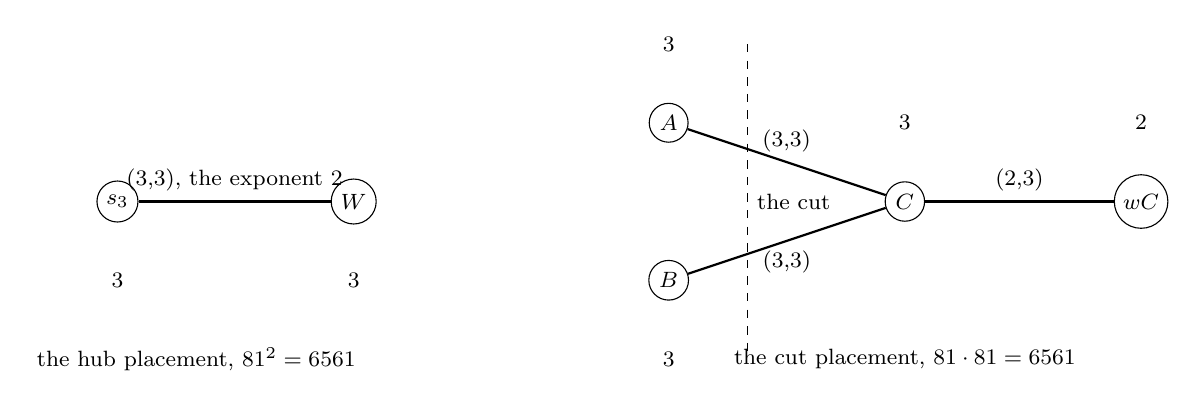
\begin{tikzpicture}[every node/.style={font=\footnotesize}]
\node[circle,draw,inner sep=2pt] (h) at (0,0) {$s_3$}; \node at (0,-1) {$3$};
\node[circle,draw,inner sep=2pt] (w) at (3,0) {$W$}; \node at (3,-1) {$3$};
\draw[thick] (h) -- node[above] {(3,3), the exponent 2} (w);
\node at (1,-2) {the hub placement, $81^2 = 6561$};
\node[circle,draw,inner sep=2pt] (a) at (7,1) {$A$}; \node at (7,2) {$3$};
\node[circle,draw,inner sep=2pt] (b) at (7,-1) {$B$}; \node at (7,-2) {$3$};
\node[circle,draw,inner sep=2pt] (c) at (10,0) {$C$}; \node at (10,1) {$3$};
\node[circle,draw,inner sep=2pt] (d) at (13,0) {$wC$}; \node at (13,1) {$2$};
\draw[thick] (a) -- node[above] {(3,3)} (c); \draw[thick] (b) -- node[below] {(3,3)} (c); \draw[thick] (c) -- node[above] {(2,3)} (d);
\draw[dashed] (8,2) -- node[right] {the cut} (8,-2);
\node at (10,-2) {the cut placement, $81\cdot 81 = 6561$};
\end{tikzpicture}
\caption{The one register at its two placements. At the hub the W word attaches at the site $s_3$ of dimension 3 by one (3,3) link read to the exponent 2. At the horizon the cut severs the two dark (3,3) links from $A$ and $B$ to the star site $C$, beside the (2,3) read tether to the dock $wC$; the product of the two wholes is the same cell.}
\end{figure}
\section{The abundances and the rate at the horizon}\label{mod:X-3-D543792-abrh-t1}
\begin{chtheorem}[The abundances and the rate at the horizon]\label{box:X-3-D543792-abrh-t1:1}
The shares of the termination census are exact rationals at every rung of the horizon web and the growth per tick is an exact element at every step, with the depth-of-the-universe open result an instance at the budget rung and the horizon web re-met at every rung at the kind under the depth rule: at the reading adopted the horizon web at rung 0 is the universe web of 444 sites, 551 links, 27 components and 36 bodies, at rung 1 the 792 webs of its first wave and at rung 2 the 37274 webs of its cut wave, a carried stretch at the rung the budget names, the tick along the parent column equal to the printed wave at 38067 of 38067 and the kind under the depth rule equal to the depth-rule entry at 38066 of 38066 webs, the join kind at 31 webs; the dock-free share at the components pooled reads 26 over 27, 19994 over 20791 and $233\,459$ over $243\,015$ at the count, the charged share 13 over 27, 10218 over 20791 and 79959 over $162\,010$, the bright share 4 over 27, 3178 over 20791 and 16169 over 97206, every one an exact rational compared with nothing; the growth per tick is an exact element at every step, the register at the rank face falling by $2^{2609}\cdot 3^{471}$ over the 792 steps of rung 1 and by $2^{127\,396}\cdot 3^{21350}$ over the 37274 steps of rung 2, the register sum down by 6631 and by $318\,842$; the processed count of the cut wave at the growth table of the horizon-depth entry, 45 against 46 distinct parents, is printed beside, and the uncapped-genre reading parts at rung 1 at the genre (2,3).
\end{chtheorem}
\chstanding{theorem}
\chdeps{Definitions 1.1 to 1.6, Theorems 99.1 and 99.2, Open results 99.3 and 99.4, Theorem 99.5 and Open result 99.6, Theorems 105.1 and 105.2, Open results 105.3 to 105.5 and Theorem 105.6 and Open results 245.1 and 245.2, Theorem 245.3, Open results 245.4 to 245.8 and Theorem 245.9}{no theorem beyond it at this release}
The universe web is parsed from the hand-off and the recorded webs of its saturation are read from the state files at every rung the budget reaches, the shares of the termination census are taken at the bodies pooled at each rung at two census readings and two weightings, and the growth per tick is read at every step at three register faces and by genre. The abundances at the horizon are exact at every recorded rung and the rate is an exact register decrease under the removing moves, the horizon web re-met at every rung at the kind under the depth rule. The horizon, the depth and the saturation stand at their own chapters.
\begin{chbridge}
In cosmology the abundances of the species are fixed at an epoch by the expansion rate and the reaction rates, the primordial abundances following from the first minutes and the expansion rate from the content, and both are measured \cite{Alpher1948,Hubble1929,Friedmann1922}. The correspondence is by name.
\end{chbridge}
\begin{chproof}[exhaustive census with its exact part]
\textit{The premises.} The axiom and the six definitions of Section~\ref{mod:FRAMEWORK}, definitions. The horizon at every rung of Section~\ref{mod:X-3-horizon-at-every-rung-and-the-horizon-web-as-a-seeded-saturation}, a theorem. The depth as the growth order and the termination wave of Section~\ref{mod:X-4-depth-the-growth-order-and-the-termination-wave}, open results. The saturation with its seeds, waves and termination of Section~\ref{mod:I-5-saturation-in-one-figure-seeds-waves-termination-sinks}, a theorem. The chain from the axiom to this result is five chapters deep.

\textit{The census.} The set counted is the recorded webs of the saturation of the horizon web at the reading adopted, the universe web at rung 0 with the genres 85, 34, 229, 134, 67 and 2 and the 792 webs of rung 1 and the 37274 webs of rung 2, 38067 webs in all, and the 35755 of the reading beside. The property tested at every web is its tick along the parent column at one move per step, equal to the printed wave at 38067 of 38067, and its kind under the depth rule equal to the depth-rule entry at 38066 of 38066. The shares at a rung are taken at the bodies of the webs recorded at the rung pooled, the components of the webs, by the census rule of the termination theorem, the membership vector over the six genres: at the count the dock-free share reads 26 over 27 at the 27 bodies of rung 0, 19994 over 20791 at the 20791 bodies of rung 1 and $233\,459$ over $243\,015$ at the $972\,060$ bodies of rung 2, at the unit weights summed the dock-free share reads 806 over 829 at rung 0; the smallest case is rung 0, 27 components of which 26 carry no dock, worked at the figure, the one dock the open dock of the universe web. The growth per tick at every step is the increase of the membership vector by genre and of the register at the three faces, defined at 792 of 792 and 37274 of 37274 steps; summed over rung 1 the net growth by genre reads $-670$, $+419$, $-2214$, $+71$, $-542$, $-72$ with the rank face $-2609$ at 2 and $-471$ at 3, and over rung 2 the rank face $-127\,396$ and $-21\,350$, the removing moves of the saturation lowering the registers at every face but the cut face at the prime 2. The depth-of-the-universe open result is an instance at the budget rung 2, and the uncapped-genre reading parts at rung 1 at the genre (2,3). So the rules pinned ahead read face A yes and face B no, the deciding letter re-lettered at zero freedom at the return from the engine readings at a table id mapped at the single-kind ids. The result is certified at the repository.

\textit{The check.} The rungs widened by one, the rung 1 struck, the (3,3) share in place of the dock-free and the (2,4) links struck each move the cells they name with the face standing where pinned, 4 of 4. The controls read the same at 10 of 11, the one that differs a processed count of the cut wave at 45 against 46 distinct parents, named beside and deciding no grade. The result was reproduced by an independent route, two engines of different construction agreeing at every cell with the runs identical beyond the header line.
\chcert{38067}
\end{chproof}
\begin{figure}[h]
\centering
\begin{adjustbox}{max width=\linewidth}\begin{tabular}{rrrl}
\hline
rung & bodies & without a dock & the dock-free share \\
\hline
0 & 27 & 26 & $(27 - 1)/27 = 26/27$ \\
1 & 20791 & 19994 & $19994/20791$ \\
\hline
\end{tabular}\end{adjustbox}
\caption{The smallest case, rung 0: 27 components of which 26 carry no dock, the one dock the open dock of the universe web; rung 1 beside.}
\end{figure}
\par\medskip\noindent{\itshape The horizon placed, the next chapter reads the depth beneath it.}\label{narr:close:10-3}\par
\section{Depth: the growth order and the termination wave}\label{mod:X-4-depth-the-growth-order-and-the-termination-wave}
\chdesig{6-4}{10-4}{X-4-depth-the-growth-order-and-the-termination-wave}{X-4-D544119-w-pwcd}
\label{narr:open:10-4}Theorem~105.1 reads depth as passage length, Theorem~105.2 the conservation of the depth fraction, Theorem~105.6 the depth independence at the sinks, and the open results Open result~105.3, Open result~105.4 and Open result~105.5 state the growth order, the termination wave and the depth at the deepest sink.
\begin{chconditional}[Depth as passage length]\label{box:X-4-depth-the-growth-order-and-the-termination-wave:1}
Conditional on the results this entry rests on, each at its own standing. The depth of a read is its passage length under the construction adopted, the passage extended beyond the open dock by a new read pair to a fresh frame at every step, the step along the tether forced by the passage parents, the depth-law cells the same under both genre faces; the theorem holds under that construction as a hypothesis and under the (2,3) genre face at the qubit far ends.
\end{chconditional}
\chstanding{conditional theorem}
\chdeps{Definitions 1.1 to 1.6, Theorems 18.1 to 18.4 and Open results 18.5 and 18.6, Open results 241.1 and 241.2, Theorems 241.3 and 241.4 and Open results 241.5 to 241.7 and Open results 245.1 and 245.2, Theorem 245.3, Open results 245.4 to 245.8 and Theorem 245.9}{the theorems of Chapters 1-4, 4-1, 5-15, 6-3 to 6-4, 6-7a}
\begin{chconditional}[Depth fraction conservation]\label{box:X-4-depth-the-growth-order-and-the-termination-wave:2}
Conditional on the results this entry rests on, each at its own standing. The ten readouts under one depth step keep their register fraction, the numerator and the denominator scaling together, while the register count moves by the whole register, the same under the cut rung and the step down; the conservation is an identity given the step and the identity carry of the readout on the free rung, two premises typed by no result, and not a law of the axiom.
\end{chconditional}
\chstanding{conditional theorem}
\chdeps{Definitions 1.1 to 1.6, Theorems 18.1 to 18.4 and Open results 18.5 and 18.6, Open results 241.1 and 241.2, Theorems 241.3 and 241.4 and Open results 241.5 to 241.7 and Open results 245.1 and 245.2, Theorem 245.3, Open results 245.4 to 245.8 and Theorem 245.9}{the theorems of Chapters 1-4, 4-1, 5-15, 6-3 to 6-4, 6-7a}
\begin{chwall}[Depth: the growth order and the termination wave]\label{box:X-4-depth-the-growth-order-and-the-termination-wave:3}
The exponents at the valence face and at the cap face are the readable spare of the universe web at the two bounds, re-derived from the hand-off and re-met, the docking-lemma count that exponent computed once more; but no result fixes the attachment site, so the depth of the horizon read is not fixed. Face A, at least one candidate reading of the attachment site equal to the exponent the derived objects carry, is met. The docking-lemma face iterated to its saturation counts sixty-three at the valence face and four hundred and thirty-two at the cap face, equal to the exponents at every derived cell. Face B, the derivation fixing no one count, is met too, and the parting is named. The three readings of the attachment site give three results, zero and one at the closure-site face, unbounded at the open-end face and sixty-three and four hundred and thirty-two at the docking-lemma face, and the face at which the horizon register is read is fixed by no result, so the depth stands here as a reading carried.
\end{chwall}
\chstanding{open result}
\chdeps{Definitions 1.1 to 1.6, Theorems 18.1 to 18.4 and Open results 18.5 and 18.6, Open results 241.1 and 241.2, Theorems 241.3 and 241.4 and Open results 241.5 to 241.7 and Open results 245.1 and 245.2, Theorem 245.3, Open results 245.4 to 245.8 and Theorem 245.9}{the theorems of Chapters 1-4, 4-1, 5-15, 6-3 to 6-4, 6-7a}
\begin{chwall}[Depth as the growth order of the closure]\label{box:X-4-depth-the-growth-order-and-the-termination-wave:4}
The growth order of the closure is re-met cell for cell and equals the depth coordinate at some readings and not at others, and the horizon count is not a function of the growth order at any closure.
\end{chwall}
\chstanding{open result}
\chdeps{Definitions 1.1 to 1.6, Theorems 18.1 to 18.4 and Open results 18.5 and 18.6, Open results 241.1 and 241.2, Theorems 241.3 and 241.4 and Open results 241.5 to 241.7 and Open results 245.1 and 245.2, Theorem 245.3, Open results 245.4 to 245.8 and Theorem 245.9}{the theorems of Chapters 1-4, 4-1, 5-15, 6-3 to 6-4, 6-7a}
\begin{chwall}[The depth at the deepest sink]\label{box:X-4-depth-the-growth-order-and-the-termination-wave:5}
The depth at the deepest sink is bounded below by the cut wave and fixed by no sink: the deepest sink of the site-bounded closure lies at the cut wave and that of the clean twin at its own, the horizon web is a sink of neither, so the depth is at least four at the first closure and at least five at the twin.
\end{chwall}
\chstanding{open result}
\chdeps{Definitions 1.1 to 1.6, Theorems 18.1 to 18.4 and Open results 18.5 and 18.6, Open results 241.1 and 241.2, Theorems 241.3 and 241.4 and Open results 241.5 to 241.7 and Open results 245.1 and 245.2, Theorem 245.3, Open results 245.4 to 245.8 and Theorem 245.9}{the theorems of Chapters 1-4, 4-1, 5-15, 6-3 to 6-4, 6-7a}
\begin{chconditional}[The depth independence at the sinks]\label{box:X-4-depth-the-growth-order-and-the-termination-wave:6}
Conditional on the results this entry rests on, among them the depth at the deepest sink, each at its own standing. The sink status of every particle web is a function of its sites and links alone: the sink letters re-derived at the stop condition equal the letters the closures typed at every web, no pairing-move edge leaves a parent typed as a sink, and no web changes its sink status with the wave or the cap, the depth part of the bound word dissolved at the sinks.
\end{chconditional}
\chstanding{conditional theorem}
\chdeps{Definitions 1.1 to 1.6, Theorems 18.1 to 18.4 and Open results 18.5 and 18.6, Open results 241.1 and 241.2, Theorems 241.3 and 241.4 and Open results 241.5 to 241.7 and Open results 245.1 and 245.2, Theorem 245.3, Open results 245.4 to 245.8 and Theorem 245.9}{the theorems of Chapters 1-4, 4-1, 5-15, 6-3 to 6-4, 6-7a}
The passage of a read is extended step by step beyond the open dock and its length compared with the depth-law cells under both genre faces. Every readout is carried through one depth step by the distributive law of the trace over a tensor product and the fraction and the count read at the free rung, the cut rung and the step down. The sink letters are re-derived from the sites and links at the stop condition and compared with the letters the closures typed. The three open questions each read the depth and find it fixed by no result. The depth of the horizon read is fixed by no result at the attachment site, the depth coordinate equals the growth order at some readings only, and the depth at the deepest sink is a bound, the termination wave of the horizon web standing at the horizon chapter as a lower bound.
\begin{chbridge}
Two terms of this chapter stand beyond the framework, each defined at its first use, \rosetta{the register tower}{a tower of Hilbert spaces of growing dimension} and \rosetta{the depth metric}{a metric on a lattice}. The correspondence is by name.
\end{chbridge}
\begin{chproof}[finite computation with its census and its exact part]
\textit{The premises.} The axiom and the six definitions of Section~\ref{mod:FRAMEWORK}, definitions. The Born count of Section~\ref{mod:I-3-records-reads-and-the-born-count-the-gain-lemma}, a theorem. The moves of Section~\ref{mod:I-4-moves-in-one-table}, definitions. The saturation of Section~\ref{mod:I-5-saturation-in-one-figure-seeds-waves-termination-sinks}, a theorem. The depth scale at the register tower, the horizon at every rung, the horizon register face at the closure, the cosmological term at the depth exponent and the horizon rung count from saturation, theorems. The universe web, a material by hash. The chain from the axiom to this result is five chapters deep.

\textit{The exact part: the readable spare at one face.} The universe web derived has 444 sites and 551 links with 54 sites of degree one and the one open dock on its tether to the closure site of dimension three at degree three. The readable spare at a bound is the count of the readable spare directions over the sites admitted at that bound. From the sites of dimension two and three admitted at the valence bound, by summation, we obtain
\begin{equation} \adjustbox{max width=\dimexpr\linewidth-3em\relax}{$\displaystyle \begin{gathered} 63 = 51 + 12\quad\text{over 60 sites at the valence face}, \\ 432 = 293 + 139\quad\text{over 369 sites at the cap face}, \end{gathered}$} \end{equation}
listed at the figure, and these are the exponents the derived objects carry at every one of 16 derived cells at each face, re-met. The smallest instance is the one-link model, whose docking-lemma count is $3$ at the valence face and $5$ at the cap face (and $1$ and $2$ at the closure-site face), checked by hand.

\textit{The finite computation.} The input objects are the three readings of the attachment site of the horizon result at the library and at the one-link model. The enumeration rule iterates each reading to its first refusal or its saturation at each bound. The closure-site face, the tether duplicated, gives $0$ at the valence face and $1$ at the cap face to its first refusal. The open-end face, the chain grown at the open end, is unbounded at both faces, admitted at every rung to five hundred. The docking-lemma face, iterated to the saturation with the walk stopped at every readable site at both orders, gives $63$ and $432$, with the mixed faces of the tower $190$ and $305$, the count face $6$ and the order depth $1$ beside, and the un-joined library $81$ and $459$. The test applied is equality with the derived exponent. The docking-lemma count equals it at both faces, because it is that exponent, the saturation count, computed once more. The three objects at it (the ladder object, the whole register to the depth, the tower object, the cut multiplied by it, and the cosmological term, one over the ladder) are exact and equal to the derived objects at 101 of 101 re-meets. The second test, whether the derivation fixes one count, reads no. The three readings give three results and no derived result fixes the attachment site.

\textit{The census.} The set counted is the derived cells carrying the exponent across the entries, 16 at each face. The property tested is equality with the readable spare re-derived from the hand-off, 16 of 16 and 16 of 16, each typed a count of the construction, and the identification of that count with the depth exponent of the horizon read typed a reading carried. The bounds at both faces (the site bound $129$ and $1165$, the free-direction bound $63$ and $507$, the closure saturated at the first and strict at the second) equal the derived cells. The sink status of every particle web, beside, is a function of its sites and links alone. The sink letters re-derived at the stop condition equal the letters the closures typed at every web.

\textit{The check.} Taking another reading of the attachment site, another bound, another order of the walk and another register each move the count they name. Striking the text moves every cell. The result was reproduced by an independent route, two engines of different construction agreeing at every cell at both runs, with the consumed files at 35 of 35 hashes and the six registers of the depth-scale result at 6 of 6 as the controls.
\chcert{101}
\end{chproof}
\begin{figure}[h]
\centering
\begin{adjustbox}{max width=\linewidth}\begin{tabular}{lllll}
\hline
face & sites admitted & spare at the qubit sites & spare at the qutrit sites & the exponent \\
\hline
the valence face & 60 & 51 & 12 & 63 \\
the cap face & 369 & 293 & 139 & 432 \\
\hline
\end{tabular}\end{adjustbox}
\caption{The readable spare of the universe web at the two bounds. At the valence face sixty-three over sixty sites and at the cap face four hundred and thirty-two over three hundred and sixty-nine sites, the exponents the derived objects carry, re-derived from the hand-off.}
\end{figure}
\section{The depth and the cap count at a larger budget}\label{mod:X-4-D540569-w-tlgc}
\begin{chwall}[The depth and the cap count at a larger budget]\label{box:X-4-D540569-w-tlgc:1}
Face A, the valence census of the universe web terminating at an exact wave at which a depth cell of the depth entries compares equal or the bound is attained, is met at no piece. Face B, the census terminating at an exact wave beneath the lower bound or beneath the depth at every reading of open, is met at no piece either. At a piece budget widened from 40 to 240 the valence census resumed from the last state of the widened census stays unterminated within the larger budget: the same three links that were open at the carried stretch stay open at every one of the 200 pieces beyond it, 548 of 551 links are capped by wave 1 and the changes per wave read 63 then 0, wave 2 is run to the 83rd of its 792 frontier webs with 84680 webs recorded, so the larger budget is exhausted first, the terminating wave stays a lower bound 1, and the comparison with the depth, a lower bound 3 fixed by no entry, stays undecided at a budget a factor of six over the widened one; the key, shared and key-and-shared readings are re-met at their terminating waves 0, 1 and 1, the depth exceeding them by at least 3, 2 and 2, and the register growth at the capped links reads 16986 at wave 1 and 0 at wave 2.
\end{chwall}
\chstanding{open result}
\chdeps{Definitions 1.1 to 1.6, Theorems 99.1 and 99.2, Open results 99.3 and 99.4, Theorem 99.5 and Open result 99.6, Theorems 105.1 and 105.2, Open results 105.3 to 105.5 and Theorem 105.6 and Open results 245.1 and 245.2, Theorem 245.3, Open results 245.4 to 245.8 and Theorem 245.9}{no theorem beyond it at this release}
The saturation of the universe web is resumed from the last state of the widened run and carried 200 pieces beyond it at the reading of open that keeps every end with spare valence open, the carried stretch re-derived equal to the widened run at every state and the three positions of the return of that run, the 96th, 99th and 101st frontier webs, lying beyond the 83rd reached. The result is an instrument of the waves run, a budget letter deciding neither face, and the same census at a still larger budget is the one further path recorded. The depth as a growth order and the termination wave stand at their own chapters.
\begin{chbridge}
A cosmological horizon in the literature is the boundary of the region a signal can reach in a finite span, and the question whether an expanding region closes or grows without bound is answered by the sign of its curvature and the content it carries \cite{Friedmann1922,HawkingEllis1973}. The correspondence is by name.
\end{chbridge}
\begin{chproof}[finite computation with its census]
\textit{The premises.} The axiom and the six definitions of Section~\ref{mod:FRAMEWORK}, definitions. The saturation with its seeds, waves and termination of Section~\ref{mod:I-5-saturation-in-one-figure-seeds-waves-termination-sinks}, definitions and a theorem. The depth as the growth order and the termination wave of Section~\ref{mod:X-4-depth-the-growth-order-and-the-termination-wave}, open results. The horizon web at the cap of Section~\ref{mod:X-3-horizon-at-every-rung-and-the-horizon-web-as-a-seeded-saturation}, an open result. The chain from the axiom to this result is five chapters deep.

\textit{The procedure.} The input is the last state of the widened run, the universe web of 444 sites and 551 links seeded at wave 0 with 497 links at their cap and 54 uncapped, resumed at the valence reading, under which an end stays open while it carries spare valence. A piece processes frontier webs in the fixed order, admitting at most 1200 canonical candidates per piece as the depth run and the widened run admitted them, so that the carried stretch is re-met piece for piece; the budget is 240 pieces per chain against 40 at the widened run, the web budget $288\,000$, the wave bound 8 and the leaf bound 4000. The test applied at each wave is the cap status of every link, a link capped once its register reaches the sum of its end sets; the stop rule fires when no link is uncapped. The aggregation is the histogram of first capping waves and the register sum at the capped links per wave.

\textit{The totals.} The carried stretch, the seed state and the 39 pieces of waves 1 and 2 of the widened run, is re-derived equal byte for byte at 160 of 160 states over both engines and both runs, the cut piece re-run whole and equal at every line beyond the budget keys, the 82 captures equal cell for cell. Beyond the carried stretch the 200 new pieces reach the 83rd frontier web of the 792 of wave 2 at the candidate 541, with the webs by wave
\begin{equation}
0:1,\qquad 1:792,\qquad 2:83887,
\end{equation}
84680 webs recorded, the totals over the chain $576\,862$ candidates, $286\,939$ admitted and $1\,018\,276$ removed. The first capping histogram reads 485 at wave 0, 63 at wave 1 and 0 at wave 2, the capped count 485, 548 and 548 and the uncapped count 66, 3 and 3 by wave, so the changes per wave are 63 then 0 and the three links open at the budget are the two hub-to-core pairs of the bodies 1 and 11 at the register 34 and the core-to-star link of the body 14 at the register 23. The register at the capped links grows by genre at wave 1 by
\begin{equation}
252 + 690 + 8772 + 936 + 6336 + 0 = 16986
\end{equation}
over the six genres from $493\,813$ to $510\,799$ and by 0 at wave 2, at two routes equal. The smallest instance is the shared reading at wave 1, re-met here: 54 uncapped links at the seed, every one capped at wave 1, the register growing by $11\,394$, the terminating wave 1; the key reading terminates at wave 0 with 221 capped and 330 fixed uncapped and the key-and-shared reading at wave 1. Against the depth, a lower bound 3 at the raised budget, the terminating waves 0, 1 and 1 fall short by at least 3, 2 and 2 and the valence reading stays undecided, so the rule pinned ahead reads face A no, face B no and the budget letter yes.

\textit{The check.} The seed struck to the one root link, the reversal cut removed, the junction move removed and the text struck each move the cells they name, the census run from the electron web of known depth terminates at its own wave and reads equal at every reading, the positive control, and the carried stretch re-run equals the widened run at 82 of 82 captures. The controls read the same at 17 of 17 beyond the two engine spellings carried as parting by construction, the chain-summing identities re-posed at the cap-wave carried stretch at 4 of 4 among them. The result was reproduced by an independent route, two engines of different construction agreeing at every cell at both runs.
\chcert{84680}
\end{chproof}
\section{The depth rule as the dynamics}\label{mod:X-4-D543100-w-prdd}
\begin{chwall}[The depth rule as the dynamics]\label{box:X-4-D543100-w-prdd:1}
Face A, the growth order of the closure and the termination wave one object under the two moves of the depth rule as the forces open result names them, the evolution at one step per tick with the advance of every settled configuration printed, reads no. Face B reads yes with the first parting named: the growth order counts the acts of the pair ket from the root, 582 attaches at every genre, 432 hub acts adding four sites and 94 joins at equal genres, and the termination wave counts the reverses of the table from the universe web, $31\,412$ reverse cuts, the reverse hub steps and 9 reverse attaches, with the 92 joins within the web, each equal to its own tick count along its parent column at every one of 1113 and 73822 webs, while the two moves of the rule, the hub-forming pairing and the (2,2) join, advance 67 of 1108 closure webs and 31 of 38066 and 31 of 35754 recorded webs; the first parting at the closure is the root qubit docked with a second qubit, the first closure at its first join at the web 2 at order 1 under an attach at the genre (2,2), an advance of neither the rule nor the table, and at the termination wave the web 10 at wave 1 under the reverse attach; under every move of the table at one step per tick the termination wave is one object with the table at every recorded web and the closure parts at the same first web with 186 equal-genre attaches and 432 hub acts of another alphabet. Beside, at the site bound six of the closure without caps, the admission clause of the rule struck: from the six genre links the closure with the two attaches at the equal genres admitted among the twenty-eight moves runs to exhaustion at 589 webs over eleven waves with twenty-five sinks at the move set and reaches six of the catalogued webs, among them the up quark bare and docked, the gluon word and the Higgs word, while the closure with the clause in force runs to exhaustion at 84 webs over eight waves with no sink and reaches five of them, the gluon word never; the ruled closure is contained in the struck at 84 of 84, the sinks part at twenty-five against none and the reached webs at the gluon word, four qutrits over three (3,3) links, twenty-six partings in all, the first a web of four sites at three links reached through the attach at the genre (3,3), present at the struck closure as an open state of the closure without caps and absent at the ruled.
\end{chwall}
\chstanding{open result}
\chdeps{Definitions 1.1 to 1.6, Theorems 105.1 and 105.2, Open results 105.3 to 105.5 and Theorem 105.6, Open results 241.1 and 241.2, Theorems 241.3 and 241.4 and Open results 241.5 to 241.7 and Open results 245.1 and 245.2, Theorem 245.3, Open results 245.4 to 245.8 and Theorem 245.9}{no theorem beyond it at this release}
The two depth open results are transcribed at their cells and re-derived along their parent columns, the depth rule is carried at its move table with its two electromagnetic moves re-met at the forces table, and the advance of every settled configuration is printed step by step under the two moves and under the whole table. The two open results are two alphabets, the acts of the pair ket and the reverses of the table, and one object not. The depth and the move table stand at their own chapters.
\begin{chbridge}
In the literature the dynamics of a system is one rule applied one step per unit of the clock, a Hamiltonian flow or a cellular automaton, and the depth of a configuration is the number of steps from the initial state under that rule \cite{Newton1687,Weinberg1995}. The correspondence is by name.
\end{chbridge}
\begin{chproof}[exhaustive census]
\textit{The premises.} The axiom and the six definitions of Section~\ref{mod:FRAMEWORK}, definitions. The depth as the growth order and the termination wave of Section~\ref{mod:X-4-depth-the-growth-order-and-the-termination-wave}, open results. The moves in one table of Section~\ref{mod:I-4-moves-in-one-table}, definitions. The saturation with its seeds, waves and termination of Section~\ref{mod:I-5-saturation-in-one-figure-seeds-waves-termination-sinks}, a theorem. The chain from the axiom to this result is four chapters deep.

\textit{The census.} The set counted is the settled configurations of the two open results: the five closures of the pair ket at 1113 webs, with the orders by closure 1 then 3 at the first, 1, 3, 1 at the second, 1, 5, 18, 79, 300, 101 at the third, 1, 5, 20, 91, 371, 16 at the fourth and four webs at every order from one to twenty-three with three at twenty-four at the fifth, and the 73822 recorded webs of the saturation of the universe web at its two readings, 38067 at the first with the webs by wave 1, 792 and 37274 and 35755 at the second with 1, 738 and 35016. The order of every web and the wave of every web are re-derived along the parent column, a root at 0 and a child one beyond its parent, equal to the printed cells at 1113 of 1113 and 73822 of 73822. The rule is carried at its cells: the move table of 28 moves, 10 adding, 10 removing and 8 keeping the site count, closed under the inverse at 14 of 14 pairs, the move-tick map zero at 9 of 9 moves and the depth increment zero at 8 of 8, and the two moves the forces open result names at the electromagnetic, the hub-forming pairing adding two sites at 16 edges of the sinks and the (2,2) join keeping the site count at 31325 edges. The property tested at every configuration is the move or act by which it advances from its parent and its kind under the rule, the two moves against the rest. At the closure the 1108 advances read 582 attaches, 179 at (2,2), 194 at (2,3), 195 at (2,4), 7 at (3,3) and 7 at (3,4), 432 hub acts at the site delta 4 and 94 joins, 67 at (2,2), 23 at (3,3) and 4 at (4,4); at the termination wave the 38066 advances of the first reading read 31 (2,2) joins, 61 (3,3) joins, 1866 reverse (3,3) joins, 9 reverse attaches, $31\,412$ reverse cuts, 1047 reverse hub pairings, 2544 reverse hub doublings, 323 reverse hub returns and 773 reverse hub steps at a kept leg, and the 35754 of the second reading alike with 31 joins. Under the two moves of the rule the advances equal at
\begin{equation}
67 \text{ of } 1108,\qquad 31 \text{ of } 38066,\qquad 31 \text{ of } 35754,
\end{equation}
the first parting at the closure the web 2 of the first closure at order 1, the root qubit docked with a second qubit under an attach at the genre (2,2), a move neither of the rule nor of the table, and at the termination wave the web 10 at wave 1 under the reverse attach, a move of the table and not of the rule; under every move of the table with its inverse the termination wave equals at 38066 of 38066 and 35754 of 35754 and the closure at 922 of 1108 with the same first parting, 186 equal-genre attaches unmapped and the 432 hub acts at the delta 4 against the delta 2 of the hub-forming move. The smallest case is the first closure at its first join, the root at order 0, three webs at order 1, the second of them the first parting.

\textit{The check.} One move of the rule struck lets the advances under the rule fall to 0 at every open result, two steps per tick part the tick from the order and the wave at every web beyond the roots and the seeds, the step reversed moves the deciding cells, and every configuration taken as already terminated moves the tick to the root value at every web, 4 of 4 as pinned. The controls read the same at 11 of 11. The result was reproduced by an independent route, two engines of different construction agreeing at every cell with the runs byte-identical.
\chcert{73822}
\end{chproof}
\begin{figure}[htbp]\centering
\setlength{\unitlength}{1mm}
\begin{picture}(160,74)(0,0)
\put(0,61){\makebox(52,8){\scriptsize the tick, the attach at (2,2), tick}}
\put(58,61){\framebox(7,7){\scriptsize 2}}
\put(78,61){\makebox(10,7){\scriptsize to}}
\put(92,61){\framebox(7,7){\scriptsize 2}}
\put(108,61){\framebox(7,7){\scriptsize 2}}
\qbezier(99,64)(103,64)(108,64)
\put(96,56){\makebox(20,4){\tiny the site 2 inserted}}
\put(118,61){\makebox(42,7){\tiny at the closure alphabet alone, 1 site and 1 link added; at no row of the table}}
\put(0,45){\makebox(52,8){\scriptsize the carrier, the attach at (2,3), carrier}}
\put(58,45){\framebox(7,7){\scriptsize 2}}
\put(78,45){\makebox(10,7){\scriptsize to}}
\put(92,45){\framebox(7,7){\scriptsize 2}}
\put(108,45){\framebox(7,7){\scriptsize 3}}
\qbezier(99,48)(103,48)(108,48)
\put(96,40){\makebox(20,4){\tiny the site 3 inserted}}
\put(118,45){\makebox(42,7){\tiny A1 adds 1 site; A1I strikes it (-1)}}
\put(0,29){\makebox(52,8){\scriptsize the vacuum, the attach at (2,4) with the hub-forming move, vacuum}}
\put(58,29){\framebox(7,7){\scriptsize 2}}
\put(78,29){\makebox(10,7){\scriptsize to}}
\put(92,29){\framebox(7,7){\scriptsize 2}}
\put(108,29){\framebox(7,7){\scriptsize 4}}
\qbezier(99,32)(103,32)(108,32)
\put(96,24){\makebox(20,4){\tiny the site 4 inserted}}
\put(118,29){\makebox(42,7){\tiny A2 adds 1 site, HF adds 2 sites, the hub act 4 sites and 5 links}}
\put(0,13){\makebox(52,8){\scriptsize the closure, the join at (2,2), closure}}
\put(58,13){\framebox(7,7){\scriptsize 2}}
\put(70,13){\framebox(7,7){\scriptsize 2}}
\put(78,13){\makebox(10,7){\scriptsize to}}
\put(92,13){\framebox(7,7){\scriptsize 2}}
\put(108,13){\framebox(7,7){\scriptsize 2}}
\qbezier(99,16)(103,16)(108,16)
\put(96,8){\makebox(20,4){\tiny the link (2,2) inserted}}
\put(118,13){\makebox(42,7){\tiny J2 keeps the site count at 0; J2I strikes the link}}
\put(0,0){\makebox(160,5){\scriptsize the closure advances under the four at the recorded reading: the tick 179, the carrier 194, the vacuum 627 (the attach 195 and the hub act 432), the closure 67; the termination wave: the carrier R2 9;R1 9, the closure R2 31;R1 31}}
\end{picture}
\par\smallskip
{\scriptsize\begin{adjustbox}{max width=\linewidth}\begin{tabular}{llllll}
id & the kinds & the site action & the site delta & the class under the two moves & the move of the rule \\ \hline
A1 & attach at (2,3) & adds & 1 & other & the carrier \\
A1I & the reverse attach at (2,3) & removes & -1 & other & the carrier, the inverse \\
A2 & attach at (2,4) & adds & 1 & other & the vacuum, the attach \\
A2I & the reverse attach at (2,4) & removes & -1 & other & the vacuum, the inverse \\
HF & hub-forming & adds & 2 & hf & the vacuum, the hub-forming move \\
the inverse of HF & the reverse hub-forming & removes & -2 & hf & the vacuum, the inverse \\
J2 & join within at (2,2), join across at (2,2) & keeps & 0 & j2 & the closure \\
J2I & the reverse join within at (2,2), the reverse join across at (2,2) & keeps & 0 & j2 & the closure, the inverse \\
the hub step forward & hub step p, hub step with the kept leg, hub step r & adds & 4,3,4 & other & the hub step family beside \\
the hub step reverse & the reverse hub step p, the reverse hub step with the kept leg, the reverse hub step r & removes & -4,-3,-4 & other & the hub step family, the inverse \\
\hline
\multicolumn{6}{l}{the table at 28 moves closed under the inverse rule at 14 of 14 pairs; the electromagnetic carried by HF;J2 at the genre (2,2), HF at 16 edges and J2 at 31325 edges} \\
\end{tabular}\end{adjustbox}}
\caption{The recorded move table drawn as the rule: the table at 28 moves closed under the inverse rule at 14 of 14 pairs, its two moves at the electromagnetic the hub-forming pairing HF and the (2,2) join J2, both at the carrier genre (2,2); the four moves of the depth rule, the tick, the carrier, the vacuum and the closure, located at the table and at the act alphabet of the recorded closure: the attach at (2,2) at no row of the table and at the closure alphabet at 179 advances, the attach at (2,3) at the table at A1 and at the closure at 194 advances, the (2,4) hub act at the table at the attach A2 and at the hub-forming move HF and at the closure at 195 attaches at (2,4) and 432 hub acts, the join at the table at J2 and at 67 closure joins; the electromagnetic carried by two move classes, HF at 16 edges and J2 at 31325 edges of the recorded sinks (the photon of the literature named for the board). Each neighbourhood is drawn at the qubit end, the site the move inserts at its dimension beside the link it makes, the inverse striking them; the kinds of the table are spelled in words.}\label{fig:X-4-D543100-move-rule}
\end{figure}
\section{The seven depth readings as one object}\label{mod:X-4-D543126-w-svdq}
\begin{chwall}[The seven depth readings as one object]\label{box:X-4-D543126-w-svdq:1}
Face A, every one of the seven depth readings one object with the serial (2,2) count or its logarithm at the webs the count is carried at, reads no. Face B reads yes with the first parting named: at the universe web the count along the chain is 1 and its logarithm 1, the tower $24\cdot 36$ over the origin 24 to the base 36, and the depth-web open result reads its chain length 0 there, the horizon-closure open result its ten candidates, 0, unbounded, 63, 1, unbounded, 432, 190, 305, 45 and 1, the deepest-sink open result its bounds 4 and 5 and the register-tower open result its bounds 3, 3, 4 and 5; at the lepton webs the count is 1 at every one and the mass-ladder open result reads its index 0, 1, 2 and its momentum 1, 2, 3; the growth-order open result and the transfer-count open result name no web the count is carried at; the first parting is the depth-web open result, its chain length 0 against the count 1 and the logarithm 1 at the universe web, the whole-web count 85 beside; the open results at one object number 0 of 7, five surviving their parting and two naming no shared web.
\end{chwall}
\chstanding{open result}
\chdeps{Definitions 1.1 to 1.6, Theorems 105.1 and 105.2, Open results 105.3 to 105.5 and Theorem 105.6 and Theorems 113.1 and 113.2}{no theorem beyond it at this release}
The seven depth open results are transcribed at their deciding cells, the serial (2,2) count and its logarithm are read at every chain state of the depth-metric open result, and every depth cell at a web the count is carried at is compared with the count and with the logarithm. Seven vocabularies of depth are not one object at the (2,2) reading. The depth and the register tower stand at their own chapters.
\begin{chbridge}
In the literature the dimension of space is one number, read alike from the growth of a ball, from the spectrum of the Laplacian, from the scaling of an entropy and from the number of independent directions, every reading agreeing on three \cite{Wald1984,HawkingEllis1973}. The correspondence is by name.
\end{chbridge}
\begin{chproof}[finite computation]
\textit{The premises.} The axiom and the six definitions of Section~\ref{mod:FRAMEWORK}, definitions. The depth as the growth order and the termination wave of Section~\ref{mod:X-4-depth-the-growth-order-and-the-termination-wave}, open results. The register tower of Section~\ref{mod:X-5-register-tower-and-the-metric}, a theorem. The depth metric of the chapter titled The (2,2) genre, the pair ket, the serial link and the increment (chapter~\ref{mod:X-0-D540399-the-two-two-census-at-every-placement}, among the instruments), at its standing. The chain from the axiom to this result is five chapters deep.

\textit{The procedure.} The seven open results are transcribed at their deciding and parting cells by locator, every one a face-B cell at an open result, 51 depth cells in all: the depth-web open result at the chain length 0 at the universe web and its first refusal at k 1, the growth-order open result at the growth order of its closure webs, the transfer-count open result at the wave of its closure webs, the horizon-closure open result at ten candidates of the universe web, the deepest-sink open result at the bounds 4 and 5, the mass-ladder open result at the index and the momentum of the three leptons, and the register-tower open result at the bounds 3, 3, 4 and 5. The serial (2,2) count along the chain run is read at 40 chain states, 1 at the hub-unit pairs of the electron, the muon, the tau, the neutron and the universe web, 0 at the dock chains of the proton and the photon word, the count metric equal to 96 multiplied by the count at 80 of 80, and the logarithm of the tower over the origin 24 to the base 36 is re-derived at every chain state by two routes, exact at 40 of 40 and equal to the count. The rule pinned ahead reads a deciding depth cell equal if it equals the count or the logarithm at its web, an open result one object if every such cell is equal and it has one, no shared web at none, and parting survives otherwise.

\textit{The totals.} At the universe web the count is 1 and the logarithm
\begin{equation}
\log_{36}\frac{24\cdot 36}{24} = 1,
\end{equation}
the smallest instance worked on the page, the whole-web count 85 beside. Against them the depth-web open result reads 0, equal at 0 of its 2 deciding cells; the horizon-closure open result reads its ten candidates, equal at 2 of 10, the closure-site face 1 at the cap bound and the order 1; the deepest-sink open result reads 4, the bound 4 against 1 and 1; the register-tower open result reads 3, the bound 3 against 1 and 1; at the lepton webs the mass-ladder open result reads the index 0, 1, 2 and the momentum 1, 2, 3 against the count 1, equal at 2 of 6; the growth-order open result at the root and the docked bodies and the transfer-count open result at its closure webs name no web the count is carried at. So the open results at one object number 0 of 7, five at parting survives and two at no shared web, face A reads no and face B reads yes with the first parting the depth-web open result. The comparison of every depth cell is printed at 35 cells at the universe web and the lepton webs at k 0 with the k beyond beside.

\textit{The check.} The universe web struck from the comparison webs moves four open results to no shared web and the first parting to the mass-ladder open result, the (2,3) count in place of the (2,2) moves two open results to one object under the struck count, the shifted origin moves the depth-web open result to one object under the struck logarithm, the text struck excludes the run, and the web with no insertion moves the counts at k 1 to 3, 5 of 5 as pinned. The controls read the same at 16 of 16, among them the count-metric theorem, the depth-metric open result, the seven open results at their partings and the web identities at 10 of 10. The result was reproduced by an independent route, two engines of different construction agreeing at every cell at both runs.
\chcert{51}
\end{chproof}
\section{Open as the depth far end}\label{mod:X-4-D543900-w-opdf}
\begin{chwall}[Open as the depth far end]\label{box:X-4-D543900-w-opdf:1}
Face A, one of the two definitions of open, the first opening the smaller end or the derived opening the larger, equal to the depth-far rule at every unequal link of every settled web with the far end named at every link, reads no. Face B reads yes with the first link named: at the arrow of a link, the chain of the link read from its tail to its head, settled at every link of the web table and carried to the universe web, the far end is the smaller end, the one the first definition opens, at 3852 of the 4642 unequal links of every settled web and the larger end, the one the derived definition opens, at 248, with no far end at 542, the 295 unequal links of the sinks beyond wave zero whose link lists are not settled and 247 settled links with no arrow, by genre 384 against 48 at (2,3), 2809 against 7 at (2,4) and 659 against 193 at (3,4), so the one-definition reading reads mixed; the first link where neither holds is the second link of the first web of the table, from its hub F to its leg f1 at the genre (4,2), whose far end f1 is the smaller, the first definition having parted at the first link from the core Q to the hub F at (3,4) whose far end F is the larger; along the chain runs of the two-metrics open result the far end is the derived open end at 8 of 8 unequal run links, under the tree distance from the depth-zero site it names the first definition at 1001, the derived at 386 and no end at 2960 links of equal depth, and under the serial (2,2) count read as a depth it names no end at any unequal link; the two parents part at the photon word chain link.
\end{chwall}
\chstanding{open result}
\chdeps{Definitions 1.1 to 1.6, Theorems 9.1 to 9.7 and Open result 9.8, Theorems 28.1 and 28.2, Open results 28.3 and 28.4 and Theorem 28.5 and Theorems 105.1 and 105.2, Open results 105.3 to 105.5 and Theorem 105.6}{no theorem beyond it at this release}
Every unequal link of every settled web is typed under the two definitions of open from the dimensions alone, the two being mirrors, and the depth-far rule, the end of a link away from the depth-zero end of its chain, is read at four readings at every link and compared with the two definitions. The depth-far end at the arrow is a third reading of open, coinciding with the first definition where the hub stands first and with the derived where the core or the dock qubit stands first, so the depth fixes neither definition at every link. The link, the read and the depth stand at their own chapters.
\begin{chbridge}
In relativity the forward end of a world line is fixed by the arrow of the proper clock along it, and which of two events follows the other is decided by the orientation of the light cone, a convention at no point and a fact along every world line \cite{Minkowski1908,HawkingEllis1973}. The correspondence is by name.
\end{chbridge}
\begin{chproof}[exhaustive census with its exact part]
\textit{The premises.} The axiom and the six definitions of Section~\ref{mod:FRAMEWORK}, definitions. The link and its six genres of Section~\ref{mod:I-2-link-and-its-six-genres}, definitions. The read at a register of Section~\ref{mod:I-6-read-at-a-register-the-probe-and-the-measurement}, definitions and theorems. The depth as the growth order and the termination wave of Section~\ref{mod:X-4-depth-the-growth-order-and-the-termination-wave}, open results. The chain from the axiom to this result is four chapters deep.

\textit{The census.} The set counted is the unequal links of every settled web of this result: the 64 webs of the web table, 1691 links of which 930 unequal; the 40 chain states of the two-metrics open result, 2960 unequal links; the eight webs of the definition open results, the universe web with 330 unequal and the seven roster webs with 51; and the 88 terminated sinks of the sinks entry, 371 unequal links; 4642 unequal links in all, 4347 with settled links. The property tested at every link is the far end under the depth-far rule at four readings against the two definitions: the first definition opens an end whose dimension is less than the far dimension and the derived opens an end whose dimension exceeds it, mirrors at 4347 of 4347 settled links, the end letters of the definition open results re-met at 1262 of 1262. At the arrow, the reading adopted, the chain of a link is read from its tail to its head, the arrow equal to the end order of the link line at 1691 of 1691 and carried to the universe web at 551 of 551, with no arrow at the inserted run links, the roster webs and the sinks beyond wave zero: the far end is named at 4100 links and none at 542, and where named it is the smaller end at 3852 and the larger at 248, $3852 + 248 + 542 = 4642$, by genre 384, 48 and 75 at (2,3), 2809, 7 and 98 at (2,4) and 659, 193 and 74 at (3,4). The smallest case is the first web of the table, worked at the figure. At the chain run the far end is the derived open end at 8 of 8 unequal run links and none at 4634; at the tree distance it is the first definition at 1001, the derived at 386 and none at 2960; under the serial (2,2) count no unequal link has a far end; the two parents part at the photon word chain link alone. So the rule pinned ahead reads face A no at the mixed reading and face B yes with the first link named, and the first link where the rule names no end is the entry link of the proton chain. The result is certified at the repository.

\textit{The check.} The arrow reversed exchanges the two letters, 248 and 3852, with the deciding cell standing, the derived re-pointed to the smaller end removes the mirror and reads neither at the larger-end links, and the reading moved to the chain run or to the tree distance moves the census as printed with the deciding cell standing, 4 of 4 as pinned. The controls read the same at 10 of 10, the arrow equal to the end order at 1691 of 1691 among them. The result was reproduced by an independent route, two engines of different construction agreeing at every cell with the runs byte-identical.
\chcert{4642}
\end{chproof}
\begin{figure}[h]
\centering
\begin{adjustbox}{max width=\linewidth}\begin{tabular}{llll}
\hline
link of the first web & end dimensions & the far end & the definition that parts \\
\hline
the core Q to the hub F & 3 and 4 & F, the larger & the first \\
the hub F to the leg f1 & 4 and 2 & f1, the smaller & the derived \\
\hline
\end{tabular}\end{adjustbox}
\caption{The smallest case, the first web of the table: at its first link the far end is the larger, where the first definition parts, and at its second the smaller, where the derived parts; the first link is where neither holds.}
\end{figure}
\section{The depth rule run to the budget at the universe web}\label{mod:X-4-D544065-the-depth-rule-run-to-the-budget-at-the-universe-web}
\begin{chtable}[The depth rule run to the budget at the universe web]\label{box:X-4-D544065-the-depth-rule-run-to-the-budget-at-the-universe-web:1}
At the three rungs the budget reaches at the horizon entry, 1, 792 and 37274 webs by rung with rung 2 a carried stretch, and at the widened-budget open result, 1, 792 and 14087, the three series of the (2,2) web are printed with the continuum statements located: the ball-growth exponent of the (2,2) web as the one-exponent census over the webs, at rung 0 yes 0, no 0, short 1, at rung 1 yes 8, no 8, short 776 and at rung 2 yes 6421, no 336, short 30517; the second difference of the (2,2) count across the web, zero at every pair site at 1 web of rung 0, 776 webs of rung 1 and 30517 webs of rung 2, the value census at rung 2 reading $-1$ at 13664, 0 at $6\,243\,534$, 1 at 12888 and 2 at 388; and the modulation along the rays, the step of the (2,2) count against the parent, at rung 1 reading $-2$ at 7, $-1$ at 664, 0 at 113 and 1 at 8 and at rung 2 $-2$ at 316, $-1$ at 32241, 0 at 4694 and 1 at 23, the ray letters at rung 2 uniform 23, still 3782, varying 33469; the ball-growth open result at one exponent first holds at rung 1 and first fails at rung 1, short at rung 0; the classical-limit open result at its inverse-square form first fails at rung 2 and first holds at no rung, its linear chain form first holding and first failing at rung 2; the wave at the rule adopted first fails at rung 1 and first holds at no rung, and at the period-one reading first holds at rung 1 and first fails at rung 2.
\end{chtable}
\chstanding{instrument}
\chdeps{Definitions 1.1 to 1.6, Theorems 90.1 to 90.4, Theorems 99.1 and 99.2, Open results 99.3 and 99.4, Theorem 99.5 and Open result 99.6 and Theorems 105.1 and 105.2, Open results 105.3 to 105.5 and Theorem 105.6}{no theorem beyond it at this release}
The depth rule is run to the budget at the universe web as an instrument: at every rung the budget reaches the ball-growth exponent of the (2,2) web, the second difference of the (2,2) count and the modulation along the rays are printed from the horizon entry and the widened-budget open result, with the rung at which each continuum statement first holds or fails, every cell exact and compared with nothing. The depth, the horizon and the curvature stand at their own chapters.
\begin{chbridge}
In the continuum the dimension of space is the exponent of the growth of a ball, the Laplacian of a density vanishes where the density is harmonic, and a wave is a modulation of a field along a ray at a fixed period, three statements the literature takes as holding at every point and at every scale \cite{Wald1984,Weinberg1995}. The correspondence is by name.
\end{chbridge}
\begin{chproof}[instrument table]
\textit{The rule that produced the table.} The webs by rung are read from the rungs table of the horizon entry at its reading adopted, 1, 792 and 37274 at the rungs 0, 1 and 2 with rung 2 a carried stretch at the budget, and from the webs table of the widened-budget open result beside, 1, 792 and 14087. At every recorded web the (2,2) web is its pair links, chains and pair sites. The ball-growth exponent is the one-exponent census of the summed ball of the (2,2) web over its orders below saturation, yes where one exponent stands at a settled growth reading, no where it does not and short where the orders carry no step; the second difference is the row-sum-zero operator of the counting face on the (2,2) links applied to the count at every pair site; the modulation is the step of the (2,2) count of a web against its parent along the rays from the seed. The columns of the table below are the series, the rung and the census at the reading adopted.

\begin{center}
\begin{adjustbox}{max width=\linewidth}\begin{tabular}{lll}
\hline
series & rung & the census at the reading adopted \\
\hline
the ball-growth exponent & 0 & yes 0, no 0, short 1 \\
 & 1 & yes 8, no 8, short 776 \\
 & 2 & yes 6421, no 336, short 30517 \\
the second difference zero at every pair site & 0, 1, 2 & 1 of 1, 776 of 792, 30517 of 37274 webs \\
the modulation along the rays & 1 & $-2$ at 7, $-1$ at 664, 0 at 113, 1 at 8 \\
 & 2 & $-2$ at 316, $-1$ at 32241, 0 at 4694, 1 at 23 \\
\hline
\end{tabular}\end{adjustbox}
\end{center}

\textit{The counts of the table.} The pooled summed ball over the webs reads 170 then 340 at rung 0 with its growth readings short, $133\,276$, $266\,576$, $266\,624$ and $266\,640$ at rung 1 and $6\,270\,474$, $12\,554\,224$, $12\,580\,776$ and $12\,593\,664$ at rung 2, its growth readings not fixed; the diameter census at rung 2 reads 1 at 30517, 2 at 336 and 3 at 6421. The value census of the second difference at rung 1 reads $-1$ at 32, 0 at $133\,220$, 1 at 16 and 2 at 8 with the trace census 166 at 7, 168 at 664, 170 at 113 and 172 at 8, and the (2,2) count census at rung 2 reads 83 at 252, 84 at 26869, 85 at 9218, 86 at 912 and 87 at 23. The ray letters at rung 1 read uniform 679, still 113 and varying 0, every ray read from the seed, and the net modulation $-670$ at rung 1 and $-32850$ at rung 2 equals the net (2,2) growth of the horizon entry. The continuum statements fall as the box prints them, the ball-growth open result holding at 8 and failing at 8 of the 792 webs of rung 1 and holding at 6421 and failing at 336 of rung 2, the classical-limit open result failing at every web of rung 2 at its inverse-square form and holding at 3805 and failing at 33469 at its linear chain form, and the wave failing at every web at the rule adopted and holding at 792 of rung 1 and 3805 of rung 2 at the period-one reading; at the reading beside the one-exponent census at rung 2 reads yes 6421, no 90, short 7576. The genre beside read in place of the genre adopted, the first link of the genre struck at every web and the rays reversed each move the cells they name, and a wrong hash excludes the run, 4 of 4 as pinned; the controls read the same at 12 of 12, among them the dark ball of the universe web at every apex equal to the ball-growth open result at the diameter 14 and the radius 1, the (2,2) web of the universe web equal to the nonlinear open result at the operator applied to the count, and the net growth equal to the growth table of the horizon entry. The table was reproduced by an independent route, two engines of different construction agreeing at every cell.
\end{chproof}
\section{The area coefficient as the depth count}\label{mod:X-4-D544091-w-ardc}
\begin{chwall}[The area coefficient as the depth count]\label{box:X-4-D544091-w-ardc:1}
Face A, the area coefficient at every rung of the fixed cut equal to the rung count multiplied by the rung-one coefficient at both readings, reads no. Face B reads yes with the first rung named: at the fixed cut of the horizon web the cut register is one register at every rung, $236\,196$, the logarithm 2 log 2 plus 10 log 3, and the coefficient at rung k, the hidden records over that logarithm, equals the rung count k multiplied by the rung-one coefficient 3 over the logarithm at every rung 1 to 6 of the docking order, where the hidden records grow by 3 per rung, 3, 3, 6, 9, 12, 15, 18, while at the open-end face the hidden records grow by 3 at every second rung, 3, 3, 6, 6, 9, 9, 12, so the coefficient reads 6 over the logarithm at rung 3 against the product 9 over the logarithm, the first parting; the qubit-end count reading, the hidden records 3 per qubit end, is equal at every rung at both faces, printed beside.
\end{chwall}
\chstanding{open result}
\chdeps{Definitions 1.1 to 1.6, Theorems 99.1 and 99.2, Open results 99.3 and 99.4, Theorem 99.5 and Open result 99.6 and Theorems 105.1 and 105.2, Open results 105.3 to 105.5 and Theorem 105.6}{no theorem beyond it at this release}
The area coefficient of the number entry is located and re-derived at every rung of the fixed cut at the two readings of the attachment site, the rung count behind the cut is read as the rung index and as the qubit-end count, and the coefficient at rung k is compared with k multiplied by the rung-one coefficient. At the docking order the coefficient is the depth count, and at the open-end face it is the qubit-end count multiplied by the rung-one coefficient, which parts from the rung count where a rung adds no qubit end. The area law, the horizon and the depth stand at their own chapters.
\begin{chbridge}
In the literature the entropy of a horizon per unit area is one constant, one quarter in Planck units, and the entropy grows with the area and with the depth of the region behind the horizon in one proportion \cite{Bekenstein1973,Hawking1975,Bousso2002}. The correspondence is by name.
\end{chbridge}
\begin{chproof}[finite computation with its exact part]
\textit{The premises.} The axiom and the six definitions of Section~\ref{mod:FRAMEWORK}, definitions. The area law at the cut of the chapter titled The area law at the cut (chapter~\ref{mod:X-2a-D542325-w-arlw}), an open result. The horizon at every rung of Section~\ref{mod:X-3-horizon-at-every-rung-and-the-horizon-web-as-a-seeded-saturation}, a theorem. The depth as the growth order and the termination wave of Section~\ref{mod:X-4-depth-the-growth-order-and-the-termination-wave}, open results. The chain from the axiom to this result is five chapters deep.

\textit{The procedure.} At the fixed cut of the horizon web, the cut at the slot severing the two (3,3) wires and the (2,3) tether at every rung, the cut register is the product of the wholes of the crossing links, located at the number entry at every rung 0 to 6 at the open-end face and the docking order, and its logarithm is taken formally as an exponent vector over the primes. The hidden records are read from the number entry, equal to the area-law open result at 14 of 14, and the coefficient at a rung is the hidden records over the logarithm, reduced, located at the number entry and re-derived here. The rung count behind the cut is the rung index k, the reading adopted, with the qubit ends behind the cut beside, 1, 1, 2, 2, 3, 3, 4 at the open-end face and 1, 1, 2, 3, 4, 5, 6 at the docking order. The rung-one coefficient is the coefficient at rung 1 of the same series, and the comparison cross-multiplies the formal quotients at both primes over the rungs 1 to 6 with the rung 0 named apart.

\textit{The totals.} From the two (3,3) wires at the whole 81 each and the (2,3) tether at the whole 36, by the product, we obtain the cut register and its logarithm
\begin{equation}
81\cdot 81\cdot 36 = 236\,196 = 2^{2}\cdot 3^{10}, \qquad \log 236\,196 = 2\log 2 + 10\log 3,
\end{equation}
one register at every rung of both readings, re-met at the number entry at 14 of 14 fixed-cut cells, the smallest instance worked on the page. The coefficient at the open-end face reads 3 over the logarithm at the rungs 0 and 1, 3 over its half at the rungs 2 and 3, 9 over the logarithm at the rungs 4 and 5 and 6 over its half at rung 6; at the docking order 3 over the logarithm at the rungs 0 and 1, then 3 over its half, 9 over the logarithm, 6 over its half, 15 over the logarithm and 9 over its half at the rungs 2 to 6; every one equal to the located cell at 28 of 28, the count reading the hidden records over 12 alike. The rung-one coefficient is 3 over the logarithm at both readings, the count reading 1 over 4. Against the rung count multiplied by it, 3, 6, 9, 12, 15, 18 over the logarithm, the docking order reads 3, 6, 9, 12, 15, 18 over the logarithm, equal at 6 of 6, and the open-end face reads 3, 6, 6, 9, 9, 12 over the logarithm, equal at the rungs 1 and 2 and parting at the rungs 3 to 6, the first parting at rung 3 with the coefficient 6 over the logarithm against the product 9 over the logarithm; the rung 0 reads the count 0 against the coefficient 3 over the logarithm at both readings, named apart, and the qubit-end count reading is equal at every rung at both faces. At the moving cut beside the open-end face parts at rung 3 and the docking order at rung 2 where the register moves at rung 1. So the rule pinned ahead reads face A no and face B yes with the first series of the frozen order, the open-end face at the fixed cut, parting at rung 3.

\textit{The check.} The hidden records shifted one rung move the docking series to parting at rung 2, the rung count offset by one and the rung-two coefficient in place of the rung-one each move the series to parting at rung 1, the tether struck moves the logarithm to 8 log 3, and the text struck excludes the run, 5 of 5 as pinned. The controls read the same at 10 of 10, among them the number entry re-met at its cut register and hidden records at 42 of 42, the area-law open result at its crossing ratios at 42 of 42 and the cut-register entry at 19 of 19 with the dark register 6561 at every rung. The result was reproduced by an independent route, two engines of different construction agreeing at every cell at both runs.
\chcert{28}
\end{chproof}
\begin{figure}[h]
\centering
\begin{adjustbox}{max width=\linewidth}\begin{tabular}{lr}
\hline
wire & the whole register \\
\hline
the first (3,3) wire & 81 \\
the second (3,3) wire & 81 \\
the (2,3) tether & 36 \\
the cut register, the product & $236\,196 = 2^{2}\cdot 3^{10}$ \\
\hline
\end{tabular}\end{adjustbox}
\caption{The smallest instance: the cut register as the product of the two (3,3) wires and the (2,3) tether, one register at every rung of both readings, its logarithm $2\log 2 + 10\log 3$.}
\end{figure}
\section{The depth at the chainless web as the web count}\label{mod:X-4-D544119-w-pwcd}
\begin{chwall}[The depth at the chainless web as the web count]\label{box:X-4-D544119-w-pwcd:1}
Face A, every one of the seven depth readings one object with the whole-web (2,2) count or its logarithm at the chainless web, reads no. Face B reads yes with the first parting named: at the universe web, the one chainless web a depth open result names, where the depth-web open result reads its chain length 0, the whole-web (2,2) count is 85 and its logarithm 85, the whole-web tower 24 multiplied by 36 to the 85 over the origin 24 to the base 36, and the depth-web open result reads its chain length 0 there, the horizon-closure open result its candidates 0, unbounded, 63, 1, unbounded, 432, 190, 305, 45 and 1, the deepest-sink open result its bounds 4 and 5 and the register-tower open result its bounds 3, 3, 4 and 5; the proton and the photon word are chainless at the web count 0 and named by no depth open result, and the growth-order, transfer-count and mass-ladder open results name no chainless web; the first parting is the depth-web open result, the chain length 0 against the web count 85 and its logarithm 85, the chain count 1 and its logarithm 1 beside; the open results at one object number 0 of 7; the web count meets every lower bound the deepest-sink and register-tower open results carry, printed beside and deciding nothing.
\end{chwall}
\chstanding{open result}
\chdeps{Definitions 1.1 to 1.6, Theorems 105.1 and 105.2, Open results 105.3 to 105.5 and Theorem 105.6 and Theorems 113.1 and 113.2}{no theorem beyond it at this release}
The seven depth readings are transcribed from the seven-readings entry at every cell and re-met against the open results, the whole-web (2,2) count and its logarithm are read at every chain state, and every depth cell at a chainless web is compared with the web count and its logarithm there. The seven vocabularies of depth do not become one object at the web count where no chain of photons runs, any more than at the chain count, the web count differing in meeting the lower bounds. The depth and the register tower stand at their own chapters.
\begin{chbridge}
In the literature the dimension of a region is read from the whole region and not from one path through it, the number of quanta in a region growing with its volume while the length of a path grows with its extent in one direction \cite{Wald1984,Chung1997}. The correspondence is by name.
\end{chbridge}
\begin{chproof}[finite computation]
\textit{The premises.} The axiom and the six definitions of Section~\ref{mod:FRAMEWORK}, definitions. The depth as the growth order and the termination wave of Section~\ref{mod:X-4-depth-the-growth-order-and-the-termination-wave}, open results. The register tower of Section~\ref{mod:X-5-register-tower-and-the-metric}, a theorem. The depth metric and the count metric of the chapter titled The (2,2) genre, the pair ket, the serial link and the increment (chapter~\ref{mod:X-0-D540399-the-two-two-census-at-every-placement}, among the instruments), at their standings. The chain from the axiom to this result is five chapters deep.

\textit{The procedure.} The seven readings are transcribed from the seven-readings entry at its 51 depth cells by locator, equal to the open results at 51 of 51 with the web tags, kinds and readings re-met, the comparison letter at every cell re-derived at the chain count and equal at 51 of 51, and the seven open results re-met at their partings at 7 of 7. The whole-web (2,2) count is read from the copies of the two-metrics open result at 40 chain states, 85 at the universe web, 1 at the electron web, 3 at the muon, 5 at the tau, 3 at the neutron and 0 at the proton and the photon word, equal to the (2,2) entry of the census by genre at 40 of 40, and its logarithm is the exponent of the whole-web tower over the origin 24 to the rung base 36, re-derived by two routes and exact at 40 of 40. A comparison web is chainless where a depth open result reads a chain length zero at it or its run count at k 0 is zero, the universe web by length and the proton and the photon word by run, and chained otherwise. The rule pinned ahead reads a deciding depth cell at a chainless web equal if it equals the web count or its logarithm there, an open result one object if every such cell is equal and it has one, no chainless web at none, and parting survives otherwise.

\textit{The totals.} At the universe web the web count is 85 and its logarithm
\begin{equation}
\log_{36}\frac{24\cdot 36^{85}}{24} = 85,
\end{equation}
exact, the smallest instance worked on the page, while the direct logarithm of 85 to the base 36 is inexact at the exponent 1 with the remainder 85 over 36, printed beside. Against the web count and its logarithm the depth-web open result reads 0, equal at 0 of its 2 deciding cells; the horizon-closure open result reads its ten candidates, equal at 0 of 10, the closure-site face 0 at the valence bound first; the deepest-sink open result reads the bound 4 against 85 and 85, the bounds 4 and 5 met at the web count beside; the register-tower open result reads the bound 3 against 85 and 85, the bounds 3, 3, 4 and 5 met beside; the growth-order open result at the root and the docked bodies, the transfer-count open result at its closure webs and the mass-ladder open result at the chained lepton webs name no chainless web; the proton and the photon word stand chainless at the web count 0 and its logarithm 0 and are named by no open result. The 23 comparisons at k 0 read equal at 0 of 20 deciding cells. So the open results at one object number 0 of 7, four at parting survives and three at no chainless web, face A reads no and face B reads yes with the first parting the depth-web open result.

\textit{The check.} The chainless tag struck moves every web to chained and every open result to no chainless web, the chain count in place of the web count re-reads the seven-readings comparison with the horizon-closure open result equal at 2 of 10, the (2,3) web count in place of the (2,2) moves the census count to 34, the text struck excludes the run, the web count at the inserted state moves every chain by one link, and the bounds read at or above move two open results to one object with the first parting standing, 6 of 6 as pinned. The controls read the same at 16 of 16, among them the count-metric theorem at both readings, the two-metrics open result at its census, metric and tower cells, the seven-readings entry at its 51 cells and the chainless tags at 7 of 7. The result was reproduced by an independent route, two engines of different construction agreeing at every cell at both runs.
\chcert{51}
\end{chproof}
\begin{figure}[htbp]\centering
\setlength{\unitlength}{1mm}
\begin{picture}(161,86)(0,0)
\put(4,85){\makebox(0,0)[tl]{\parbox{150mm}{\footnotesize the universe web: 85 (2,2) links at 170 pair sites, the longest (2,2) chain 1; the recorded chain B00.f1 to B00.f2 at the cell (2,2)}}}
\put(4,64){\circle{2}}\put(9,64){\circle{2}}\put(5,64){\line(1,0){3}}
\put(5,66){\makebox(0,0)[rb]{\tiny B00.f1}}\put(8,66){\makebox(0,0)[lb]{\tiny B00.f2}}\put(6,62){\makebox(0,0)[t]{\tiny (2,2)}}
\put(13,64){\circle{2}}\put(18,64){\circle{2}}\put(14,64){\line(1,0){3}}
\put(22,64){\circle{2}}\put(27,64){\circle{2}}\put(23,64){\line(1,0){3}}
\put(31,64){\circle{2}}\put(36,64){\circle{2}}\put(32,64){\line(1,0){3}}
\put(40,64){\circle{2}}\put(45,64){\circle{2}}\put(41,64){\line(1,0){3}}
\put(49,64){\circle{2}}\put(54,64){\circle{2}}\put(50,64){\line(1,0){3}}
\put(58,64){\circle{2}}\put(63,64){\circle{2}}\put(59,64){\line(1,0){3}}
\put(67,64){\circle{2}}\put(72,64){\circle{2}}\put(68,64){\line(1,0){3}}
\put(76,64){\circle{2}}\put(81,64){\circle{2}}\put(77,64){\line(1,0){3}}
\put(85,64){\circle{2}}\put(90,64){\circle{2}}\put(86,64){\line(1,0){3}}
\put(94,64){\circle{2}}\put(99,64){\circle{2}}\put(95,64){\line(1,0){3}}
\put(103,64){\circle{2}}\put(108,64){\circle{2}}\put(104,64){\line(1,0){3}}
\put(112,64){\circle{2}}\put(117,64){\circle{2}}\put(113,64){\line(1,0){3}}
\put(121,64){\circle{2}}\put(126,64){\circle{2}}\put(122,64){\line(1,0){3}}
\put(130,64){\circle{2}}\put(135,64){\circle{2}}\put(131,64){\line(1,0){3}}
\put(139,64){\circle{2}}\put(144,64){\circle{2}}\put(140,64){\line(1,0){3}}
\put(148,64){\circle{2}}\put(153,64){\circle{2}}\put(149,64){\line(1,0){3}}
\put(4,50){\circle{2}}\put(9,50){\circle{2}}\put(5,50){\line(1,0){3}}
\put(13,50){\circle{2}}\put(18,50){\circle{2}}\put(14,50){\line(1,0){3}}
\put(22,50){\circle{2}}\put(27,50){\circle{2}}\put(23,50){\line(1,0){3}}
\put(31,50){\circle{2}}\put(36,50){\circle{2}}\put(32,50){\line(1,0){3}}
\put(40,50){\circle{2}}\put(45,50){\circle{2}}\put(41,50){\line(1,0){3}}
\put(49,50){\circle{2}}\put(54,50){\circle{2}}\put(50,50){\line(1,0){3}}
\put(58,50){\circle{2}}\put(63,50){\circle{2}}\put(59,50){\line(1,0){3}}
\put(67,50){\circle{2}}\put(72,50){\circle{2}}\put(68,50){\line(1,0){3}}
\put(76,50){\circle{2}}\put(81,50){\circle{2}}\put(77,50){\line(1,0){3}}
\put(85,50){\circle{2}}\put(90,50){\circle{2}}\put(86,50){\line(1,0){3}}
\put(94,50){\circle{2}}\put(99,50){\circle{2}}\put(95,50){\line(1,0){3}}
\put(103,50){\circle{2}}\put(108,50){\circle{2}}\put(104,50){\line(1,0){3}}
\put(112,50){\circle{2}}\put(117,50){\circle{2}}\put(113,50){\line(1,0){3}}
\put(121,50){\circle{2}}\put(126,50){\circle{2}}\put(122,50){\line(1,0){3}}
\put(130,50){\circle{2}}\put(135,50){\circle{2}}\put(131,50){\line(1,0){3}}
\put(139,50){\circle{2}}\put(144,50){\circle{2}}\put(140,50){\line(1,0){3}}
\put(148,50){\circle{2}}\put(153,50){\circle{2}}\put(149,50){\line(1,0){3}}
\put(4,36){\circle{2}}\put(9,36){\circle{2}}\put(5,36){\line(1,0){3}}
\put(13,36){\circle{2}}\put(18,36){\circle{2}}\put(14,36){\line(1,0){3}}
\put(22,36){\circle{2}}\put(27,36){\circle{2}}\put(23,36){\line(1,0){3}}
\put(31,36){\circle{2}}\put(36,36){\circle{2}}\put(32,36){\line(1,0){3}}
\put(40,36){\circle{2}}\put(45,36){\circle{2}}\put(41,36){\line(1,0){3}}
\put(49,36){\circle{2}}\put(54,36){\circle{2}}\put(50,36){\line(1,0){3}}
\put(58,36){\circle{2}}\put(63,36){\circle{2}}\put(59,36){\line(1,0){3}}
\put(67,36){\circle{2}}\put(72,36){\circle{2}}\put(68,36){\line(1,0){3}}
\put(76,36){\circle{2}}\put(81,36){\circle{2}}\put(77,36){\line(1,0){3}}
\put(85,36){\circle{2}}\put(90,36){\circle{2}}\put(86,36){\line(1,0){3}}
\put(94,36){\circle{2}}\put(99,36){\circle{2}}\put(95,36){\line(1,0){3}}
\put(103,36){\circle{2}}\put(108,36){\circle{2}}\put(104,36){\line(1,0){3}}
\put(112,36){\circle{2}}\put(117,36){\circle{2}}\put(113,36){\line(1,0){3}}
\put(121,36){\circle{2}}\put(126,36){\circle{2}}\put(122,36){\line(1,0){3}}
\put(130,36){\circle{2}}\put(135,36){\circle{2}}\put(131,36){\line(1,0){3}}
\put(139,36){\circle{2}}\put(144,36){\circle{2}}\put(140,36){\line(1,0){3}}
\put(148,36){\circle{2}}\put(153,36){\circle{2}}\put(149,36){\line(1,0){3}}
\put(4,22){\circle{2}}\put(9,22){\circle{2}}\put(5,22){\line(1,0){3}}
\put(13,22){\circle{2}}\put(18,22){\circle{2}}\put(14,22){\line(1,0){3}}
\put(22,22){\circle{2}}\put(27,22){\circle{2}}\put(23,22){\line(1,0){3}}
\put(31,22){\circle{2}}\put(36,22){\circle{2}}\put(32,22){\line(1,0){3}}
\put(40,22){\circle{2}}\put(45,22){\circle{2}}\put(41,22){\line(1,0){3}}
\put(49,22){\circle{2}}\put(54,22){\circle{2}}\put(50,22){\line(1,0){3}}
\put(58,22){\circle{2}}\put(63,22){\circle{2}}\put(59,22){\line(1,0){3}}
\put(67,22){\circle{2}}\put(72,22){\circle{2}}\put(68,22){\line(1,0){3}}
\put(76,22){\circle{2}}\put(81,22){\circle{2}}\put(77,22){\line(1,0){3}}
\put(85,22){\circle{2}}\put(90,22){\circle{2}}\put(86,22){\line(1,0){3}}
\put(94,22){\circle{2}}\put(99,22){\circle{2}}\put(95,22){\line(1,0){3}}
\put(103,22){\circle{2}}\put(108,22){\circle{2}}\put(104,22){\line(1,0){3}}
\put(112,22){\circle{2}}\put(117,22){\circle{2}}\put(113,22){\line(1,0){3}}
\put(121,22){\circle{2}}\put(126,22){\circle{2}}\put(122,22){\line(1,0){3}}
\put(130,22){\circle{2}}\put(135,22){\circle{2}}\put(131,22){\line(1,0){3}}
\put(139,22){\circle{2}}\put(144,22){\circle{2}}\put(140,22){\line(1,0){3}}
\put(148,22){\circle{2}}\put(153,22){\circle{2}}\put(149,22){\line(1,0){3}}
\put(4,8){\circle{2}}\put(9,8){\circle{2}}\put(5,8){\line(1,0){3}}
\put(13,8){\circle{2}}\put(18,8){\circle{2}}\put(14,8){\line(1,0){3}}
\put(22,8){\circle{2}}\put(27,8){\circle{2}}\put(23,8){\line(1,0){3}}
\put(31,8){\circle{2}}\put(36,8){\circle{2}}\put(32,8){\line(1,0){3}}
\put(40,8){\circle{2}}\put(45,8){\circle{2}}\put(41,8){\line(1,0){3}}
\put(49,8){\circle{2}}\put(54,8){\circle{2}}\put(50,8){\line(1,0){3}}
\put(58,8){\circle{2}}\put(63,8){\circle{2}}\put(59,8){\line(1,0){3}}
\put(67,8){\circle{2}}\put(72,8){\circle{2}}\put(68,8){\line(1,0){3}}
\put(76,8){\circle{2}}\put(81,8){\circle{2}}\put(77,8){\line(1,0){3}}
\put(85,8){\circle{2}}\put(90,8){\circle{2}}\put(86,8){\line(1,0){3}}
\put(94,8){\circle{2}}\put(99,8){\circle{2}}\put(95,8){\line(1,0){3}}
\put(103,8){\circle{2}}\put(108,8){\circle{2}}\put(104,8){\line(1,0){3}}
\put(112,8){\circle{2}}\put(117,8){\circle{2}}\put(113,8){\line(1,0){3}}
\put(121,8){\circle{2}}\put(126,8){\circle{2}}\put(122,8){\line(1,0){3}}
\put(130,8){\circle{2}}\put(135,8){\circle{2}}\put(131,8){\line(1,0){3}}
\put(139,8){\circle{2}}\put(144,8){\circle{2}}\put(140,8){\line(1,0){3}}
\put(148,8){\circle{2}}\put(153,8){\circle{2}}\put(149,8){\line(1,0){3}}
\end{picture}
\caption{The universe web with its 85 (2,2) links at 170 pair sites and the longest chain one: the whole-web (2,2) count 85 and the longest (2,2) chain one, the chain the hub-unit pair carrying one (2,2) link, the web at two numbers. The census by genre of the web reads 85, 34, 229, 134, 67 and 2 at the six genres in their order, at 444 sites and 551 links; the 85 pair sites are drawn as 85 pairs, the chain named at its two sites.}\label{fig:X-4-D544119-universe-web}
\end{figure}
\par\medskip\noindent{\itshape Depth read, the next chapter reads the tower of registers and the metric it carries.}\label{narr:close:10-4}\par
\section*{The Metric And The Worldline}
\addcontentsline{toc}{section}{The Metric And The Worldline}
\section{The register tower and the metric}\label{mod:X-5-register-tower-and-the-metric}
\chdesig{6-5}{10-5}{X-5-register-tower-and-the-metric}{X-5-D542610-lgtw-t1}
\label{narr:open:10-5}Theorem~113.1 reads the register tower and the metric and Theorem~113.2 the two metrics at a corridor.
\begin{chconditional}[The register tower and the metric]\label{box:X-5-register-tower-and-the-metric:1}
Conditional on the results this entry rests on, each at its own standing. The dark-port count of the cross core is six, the pendant links of the three depth webs at two each, every one dark; the depth exponent at the count face equals that count, so the scale in the electron unit is the whole register thirty-six to the minus six, equal to the tower ratio; the register tower, twenty-four multiplied by thirty-six to the rung, equals the horizon cells at every rung and the ladder cells, and the tower and ladder objects at the horizon rung count are the exact objects at which the gravitational coupling and the expansion-rate ratio are read, and no comparison with observation is made here; the theorem holds under the posed count face, a definition of the depth exponent typed by no result.
\end{chconditional}
\chstanding{conditional theorem}
\chdeps{Definitions 1.1 to 1.6, Theorems 9.1 to 9.7 and Open result 9.8, Theorems 18.1 to 18.4 and Open results 18.5 and 18.6 and Open results 245.1 and 245.2, Theorem 245.3, Open results 245.4 to 245.8 and Theorem 245.9}{the theorems of Chapters 1-5, 5-3, 6-1, 6-2a, 6-3 to 6-6, 6-10}
\begin{chconditional}[The two metrics at a corridor]\label{box:X-5-register-tower-and-the-metric:2}
Conditional on the results this entry rests on, among them depth metric with the rung term, depth as passage length and confinement as the dark genre readability, each at its own standing. At every joined web the two mouths of every dark (3,3) pairing link stand at the dark distance of one rung and at the washed distance of none at both washed readings, the mouths in distinct washed components, so that a corridor is adjacent at the dark read and invisible at the washed read, priced by nothing in washed space and shortening nothing a dock can see.
\end{chconditional}
\chstanding{conditional theorem}
\chdeps{Definitions 1.1 to 1.6, Theorems 9.1 to 9.7 and Open result 9.8, Theorems 18.1 to 18.4 and Open results 18.5 and 18.6 and Open results 245.1 and 245.2, Theorem 245.3, Open results 245.4 to 245.8 and Theorem 245.9}{the theorems of Chapters 1-5, 5-3, 6-1, 6-2a, 6-3 to 6-6, 6-10}
The pendant links of the cross core are counted and typed dark, the depth exponent read at the count face, the scale compared with the tower ratio, the register tower compared with the horizon and ladder cells at every rung, and the tower and ladder objects formed at the rung count re-derived from the universe web. The joined webs are built from the deuteron and meson link lists and the two stars, the dark distance between the mouths of every dark pairing link read as its rung count and the washed distance read as the component structure of the washed web. What stands open is not a question of this chapter but the posed count face on which the depth scale rests, a definition typed by no result, and the open questions the corridor theorem consumes. The metric as the register tower read at the depth is the question of the last chapter of this Part.
\begin{chbridge}
Two terms of this chapter stand beyond the framework, each defined at its first use, \rosetta{the register tower}{a tower of Hilbert spaces of growing dimension} and \rosetta{the depth metric}{a metric on a lattice}. The correspondence is by name, and no coupling or expansion-rate figure is displayed here.
\end{chbridge}
\begin{chproof}[finite computation with its census and its exact part]
\textit{The premises.} The axiom and the six definitions of Section~\ref{mod:FRAMEWORK}, definitions. The link and its six genres of Section~\ref{mod:I-2-link-and-its-six-genres}, definitions. The Born count of Section~\ref{mod:I-3-records-reads-and-the-born-count-the-gain-lemma}, a theorem. The rungs of Section~\ref{mod:I-5-saturation-in-one-figure-seeds-waves-termination-sinks}, a theorem. The second-order dark read, the junction register, the one-ladder, horizon and saturation results, theorems. The boundary count from the valence law and the join from shared, open results read at their grades. The posed count face, a definition carried by name. The chain from the axiom to this result is five chapters deep.

\textit{The exact part: the scale at the count face.} The cross core of the library is the three depth webs, drawn at the figure at the first of them. They have the sites $5$, $10$ and $15$, the links $5$, $11$ and $17$, the measures $36$, $76$ and $116$, every link dark at the typing adopted (no read-genre link at any depth web). The dark ports are the pendant links at a site of degree one, two at each depth web. From the three webs, by counting, we obtain the dark-port count $6$, equal to the typed ports of the second-order dark read. The registers from the dimensions of the read genre (2,3) are the whole $36=4\cdot 9$ and the cut $24=8\cdot 3$. The depth exponent at the count face is the number of dark-port reads at the second order with a nonzero readout at the cut register, $6$ of $6$, so from the whole register and the count, by the power, we obtain the scale in the electron unit
\begin{equation}
36^{-6}=\frac{1}{2\,176\,782\,336},
\end{equation}
equal to the tower ratio at the second spelling, with the per-web scale $1/1296$ at each depth web beside. The register tower is $24\cdot 36^{k}$ at the rung $k$, equal to the Weyl cells of the horizon result at the rungs zero to six at both readings and to the ladder cells of the one-ladder result. The smallest instance is the first depth web, one hub with four (2,4) legs and one (2,2) pair, two pendant legs, the count two.

\textit{The finite computation and the census.} The input object is the universe web with its 444 sites and 551 links. The enumeration rule re-derives the horizon rung count as the readable spare, $63$ at the first valence order and $432$ at the second, equal to the saturation and horizon cells. The tower at the rung count is $24\cdot 36^{63}$ (a hundred digits) and $24\cdot 36^{432}$, and the ladder objects $36^{63}$ and $36^{432}$ with their inverses are the exact objects at which the gravitational coupling and the expansion-rate ratio are read as objects, and no comparison with observation is made here. The set counted is the re-meets of the consumed results, 214 in all, every one equal. The register faces beside read equal to the count at 2 of 20 readings (the valuation of the mass office of the second depth web at both its parts), the first differing the nesting counts of the one-ladder result, printed beside. The corridor result of the second box stands beside. At every joined web the two mouths of every dark (3,3) pairing link stand at the dark distance of one rung and at the washed distance of none, in distinct washed components.

\textit{The check.} Reading a pendant link as not dark, taking the count face at the whole register, replacing the universe web by the electron web and striking the text each move the cells they name. The result was reproduced by an independent route, two engines of different construction agreeing at 530 shared keys with none differing, with the library at its hash and census as the control.
\chcert{214}
\end{chproof}
\begin{figure}[h]
\centering
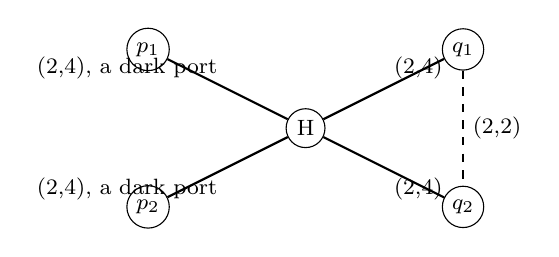
\begin{tikzpicture}[every node/.style={font=\footnotesize}]
\node[circle,draw,inner sep=2pt] (H) at (0,0) {H};
\node[circle,draw,inner sep=2pt] (p1) at (-2,1) {$p_1$};
\node[circle,draw,inner sep=2pt] (p2) at (-2,-1) {$p_2$};
\node[circle,draw,inner sep=2pt] (q1) at (2,1) {$q_1$};
\node[circle,draw,inner sep=2pt] (q2) at (2,-1) {$q_2$};
\draw[thick] (H) -- node[above left] {(2,4), a dark port} (p1);
\draw[thick] (H) -- node[below left] {(2,4), a dark port} (p2);
\draw[thick] (H) -- node[above right] {(2,4)} (q1);
\draw[thick] (H) -- node[below right] {(2,4)} (q2);
\draw[dashed] (q1) -- node[right] {(2,2)} (q2);
\end{tikzpicture}
\caption{The first depth web of the cross core. A hub H of dimension four with four (2,4) legs to qubits and one (2,2) pair, five sites and five links. The two pendant legs $p_1$ and $p_2$ at degree one are its dark ports, two of the six of the cross core.}
\end{figure}
\section{The count metric as the logarithm of the tower metric}\label{mod:X-5-D542610-lgtw-t1}
\begin{chconditional}[The count metric as the logarithm of the tower metric]\label{box:X-5-D542610-lgtw-t1:1}
Conditional on the entries this result rests on, each at its own standing. The count metric of the depth-metric open result is the logarithm of its tower metric: at every chain state of that open result the count metric, the cap 96 multiplied by the depth, equals the cap multiplied by the logarithm, to the rung base 36, of the tower metric over its origin 24, the logarithm exact at every chain state and equal to the depth, the tower the origin multiplied by the rung base to the depth, $24\cdot 36$ at every hub-unit pair at k 0, $31\,104$, $1\,119\,744$ and $40\,310\,784$ at k 1, 2 and 3 and 24 at the dock chains at k 0 where the depth is zero, equal at 28 of 28 chain states; the origin 24 equals the product of the three register dimensions 2, 3 and 4 at the dock web; the first parting of the depth-metric open result, the electron at k 0 with the tower $24\cdot 36$ against the count metric 96, is re-read equal as the origin offset, 96 multiplied by the logarithm 1 equal to 96 and at the depth zero 0 equal to 0; the unit reading beside, the base 6 and the origin 4, is exact and parts at every chain state, printed beside.
\end{chconditional}
\chstanding{conditional theorem}
\chdeps{Definitions 1.1 to 1.6 and Theorems 113.1 and 113.2}{no theorem beyond it at this release}
The tower metric and the count metric are read from the chain states of the depth-metric open result, the logarithm of the tower over its origin to the rung base is printed as an exact element at every state and compared with the count, and the origin is set beside the product of the register dimensions at the dock. The two metrics of that open result are one metric in two readings, the tower geometric and the count arithmetic, the logarithm carrying the one into the other with the origin as the offset. The register tower stands at its own chapter.
\begin{chbridge}
In statistical mechanics the entropy of a system is the logarithm of its number of states, so that a count that grows exponentially along a chain and a count that grows linearly are one quantity in two readings, and in a geometry a distance is additive while a volume multiplies \cite{Gibbs1902,Wald1984}. The correspondence is by name.
\end{chbridge}
\begin{chproof}[finite computation with its exact part]
\textit{The premises.} The axiom and the six definitions of Section~\ref{mod:FRAMEWORK}, definitions. The register tower and the metric of Section~\ref{mod:X-5-register-tower-and-the-metric}, a theorem. The depth metric and the serial link of the chapter titled The (2,2) genre, the pair ket, the serial link and the increment (chapter~\ref{mod:X-0-D540399-the-two-two-census-at-every-placement}, among the instruments), at their standings. The chain from the axiom to this result is four chapters deep.

\textit{The procedure.} The tower metric is read from the settled copies of the depth-metric open result at its ten chains and k 0 to 3, the seven chains and the three beside, at the depth readings and the tower readings, 480 cells; the rung base 36 and the origin 24 are read by locator from its rung cells, equal to the whole and the cut of the (2,3) read genre, the cut of the read genre multiplied by its whole re-met at the depth-scale entry at 48 of 48 and at the cut-register entry at 40 of 40. The logarithm of the tower over its origin to the rung base is taken as the greatest integer whose power of the base is at most the ratio, the remainder the ratio over that power, exact where the remainder is one. The count metric, the cap 96 multiplied by the depth, is compared with the cap multiplied by the exponent as an exact difference at every chain state, the first parting taken in the order of the chains and k. The origin is compared with the product of the distinct site dimensions of the dock web.

\textit{The totals.} At every chain state the tower reads the origin multiplied by the rung base to the depth, 24 at the depth 0 of the proton and the photon word at k 0, $24\cdot 36$ at the depth 1 of every hub-unit pair at k 0, and $31\,104$, $1\,119\,744$ and $40\,310\,784$ at the depths 2, 3 and 4, so the logarithm
\begin{equation}
\log_{36}\frac{24\cdot 36^{d}}{24} = d
\end{equation}
is exact at 600 of 600 cells over every reading, each tower reading geometric in its own base, and equal to the depth at 40 of 40 at the readings adopted, 0 at the dock chains, 1 at the hub-unit pairs and 2, 3, 4 at k 1, 2, 3, with 85 to 88 at the whole-web reading of the universe web. From the logarithm, by the cap, we obtain $96 d$ against the count metric $96 d$, the difference zero at every state, 0 against 0 at the depth 0, 96 against 96 at the depth 1 and 192, 288 and 384 against 192, 288 and 384 beyond, equal at 28 of 28 chain states and at every depth and tower reading at its own base, the whole-web reading 8160 against 8160 at k 0; the smallest instance is the electron at k 0, the tower $24\cdot 36$ over the origin 24 the base to the one, 96 multiplied by 1 equal to 96, which re-reads the first parting of the depth-metric open result as the origin offset. From the dock web of the electron, by its three distinct site dimensions, we obtain the origin
\begin{equation}
2\cdot 3\cdot 4 = 24,
\end{equation}
equal to the cut of the electron dock pair of the mass-unit entry with the rung base equal to its whole. The unit reading beside, four multiplied by 6 to the twice the depth plus one, is exact with the exponent twice the depth plus one and parts at every chain state, the electron at k 0 reading 96 against 288. So the rule pinned ahead reads face A yes and face B no with the first parting none.

\textit{The check.} The shifted origin moves the exponent at the electron from 1 to 0 and the deciding cell to no, the different base moves the logarithm inexact at every depth beyond zero, the (2,3) insertion in place of the (2,2) moves the depth at k 1 from 2 to 0 with the comparison standing, the text struck excludes the run, and the chain with no insertion moves every k to its k 0 state, 5 of 5 as pinned. The controls read the same at 16 of 16, among them the tower cells of the depth-metric open result at 480 of 480, its count metric at 80 of 80, the depth-scale entry at 48 of 48 and the distinct ratios 9, 162, 3888 and $104\,976$ re-derived. The result was reproduced by an independent route, two engines of different construction agreeing at every cell at both runs.
\chcert{600}
\end{chproof}
\begin{figure}[htbp]\centering
\scriptsize
\setlength{\tabcolsep}{3pt}
\begin{adjustbox}{max width=\linewidth}\begin{tabular}{llrrrrrr}
state & run & depth & tower & logarithm & cap by logarithm & count metric & difference \\ \hline
k0 & a1-a2 & 1 & eight hundred and sixty-four & 1 & 96 & 96 & 0 \\
k1 & a1-x1-a2 & 2 & 31104 & 2 & 192 & 192 & 0 \\
k2 & a1-x1-x2-a2 & 3 & 1119744 & 3 & 288 & 288 & 0 \\
k3 & a1-x1-x2-x3-a2 & 4 & 40310784 & 4 & 384 & 384 & 0 \\
\end{tabular}\end{adjustbox}
\caption{The count metric against the tower metric at the chain states of the electron web: the count metric is the cap 96 multiplied by the depth, the tower is the origin 24 multiplied by the rung base 36 to the depth, the logarithm of the tower over its origin to the rung base is the depth, and the difference between the count metric and the cap multiplied by the logarithm is zero at every state.}\label{fig:X-5-D542610-count-against-tower}
\end{figure}
\begin{figure}[h]
\centering
\begin{adjustbox}{max width=\linewidth}\begin{tabular}{rrr}
\hline
depth & $96 d$ from the logarithm & the count metric \\
\hline
0 & 0 & 0 \\
1 & 96 & 96 \\
2 & 192 & 192 \\
\hline
\end{tabular}\end{adjustbox}
\caption{The smallest instance, the electron at k 0: the tower $24\cdot 36$ over the origin 24 is the base to the one, so 96 multiplied by 1 equals 96, the origin offset of the depth-metric open result re-read; the difference zero at every depth.}
\end{figure}
\par\medskip\noindent{\itshape The next chapter reads the term the literature attaches to the vacuum.}\label{narr:close:10-5}\par
\section{The cosmological term at the depth exponent}\label{mod:X-6-cosmological-term-at-the-depth-exponent}
\chdesig{6-6}{10-6}{X-6-cosmological-term-at-the-depth-exponent}{X-6-D542582-w-tktu}
\label{narr:open:10-6}Theorem~115.1 reads the cosmological term at the depth exponent, resting on the link and the saturation.
\begin{chconditional}[The cosmological term at the depth exponent]\label{box:X-6-cosmological-term-at-the-depth-exponent:1}
Conditional on depth scale at the register tower, horizon at every rung from iterated closure and horizon register face at the closure, each at its own standing. The closure constant of the horizon register is thirty-six at every rung, the two faces of the register are related by the closure count alone, the ratio of the ladder objects at the two faces an exact power of the whole register, and one face names the term, the valence face at the closure count sixty-three equal to its free-direction bound, where the closure is saturated while the cap face is strict; so the cosmological term is an exact object at the valence face, the closure constant to the minus the depth exponent, the exact inverse of the ladder object at ninety-nine digits.
\end{chconditional}
\chstanding{conditional theorem}
\chdeps{Definitions 1.1 to 1.6, Theorems 9.1 to 9.7 and Open result 9.8 and Open results 245.1 and 245.2, Theorem 245.3, Open results 245.4 to 245.8 and Theorem 245.9}{the theorems of Chapters 1-2, 1-5, 4-1, 4-3, 5-3, 6-2, 6-6}
The closure constant of the horizon register is read at every rung of the register tower, the closure count re-derived from the universe web at the valence face and at the cap face and compared with the free-direction bound at each, the ladder objects formed at both faces and their ratio computed by exact division, and the term formed as the closure constant to the minus the depth exponent at the one face at which the closure is saturated. The cosmological term is the closure constant to the minus the depth exponent, an exact object at one reading of the horizon register, sixty-three at the valence reading and four hundred thirty-two at the cap reading, the one reading named the valence reading. What stands open is not a question of this chapter. The depth exponent at the valence face is a reading carried at a face the derivations do not fix, so the term as an exact object stands at that reading and its magnitude is not compared with observation here.
\begin{chbridge}
One term of this chapter stands beyond the framework, defined at its first use, \rosetta{the register tower}{a tower of Hilbert spaces of growing dimension}. The correspondence is by name, and no value of the term is displayed here.
\end{chbridge}
\begin{chproof}[finite computation with its exact part]
\textit{The premises.} The axiom and the six definitions of Section~\ref{mod:FRAMEWORK}, definitions. The link and its genres of Section~\ref{mod:I-2-link-and-its-six-genres}, definitions. The rungs and the horizon web of Section~\ref{mod:I-5-saturation-in-one-figure-seeds-waves-termination-sinks}, a theorem. The depth scale at the register tower of Section~\ref{mod:X-5-register-tower-and-the-metric}, a theorem under its posed count face. The horizon at every rung of Section~\ref{mod:X-3-horizon-at-every-rung-and-the-horizon-web-as-a-seeded-saturation} and the horizon register face at the closure, theorems. The join from shared, an open result consumed as a material. The chain from the axiom to this result is five chapters deep.

\textit{The exact part: the closure constant and the term.} The registers from the dimensions of the read genre (2,3) are the whole $36=4\cdot 9$ and the cut $24=8\cdot 3$. The register tower, listed at the figure, is the cut multiplied by the whole to the rung,
\begin{equation} \adjustbox{max width=\dimexpr\linewidth-3em\relax}{$\displaystyle T_k=24\cdot 36^{k}:\quad 24,\ 24\cdot 36,\ 31\,104,\ 1\,119\,744,\ 40\,310\,784,\ 1\,451\,188\,224,\ 52\,242\,776\,064\quad (k=0,\dots,6),$} \end{equation}
and from consecutive rungs, by exact division, we obtain the closure constant $T_k/T_{k-1}=36$ at every rung one to six, the law a power at the whole register. At the fixed interface the count is nine at every rung and the constant one. The closure count at each face is the readable spare of the universe web, $63$ at the valence face (over 60 sites) and $432$ at the cap face (over 369 sites). From the closure constant and the closure count, by the power, we obtain the ladder object $36^{63}$ at the valence face (an exact integer of ninety-nine digits) and $36^{432}$ at the cap face, their ratio $36^{369}$ an exact power of the whole register by exact division, so the two faces are related by the closure count alone. At the valence face the closure count $63$ equals its free-direction bound $63$, the closure saturated, while at the cap face $432$ stands against the bound $507$, strict. So the one face naming the term is the valence face, and the term is
\begin{equation}
\Lambda=36^{-63},
\end{equation}
the exact inverse of the ladder object, compared with nothing here. The smallest instance is the first rung, $(24\cdot 36)/24=36$, checked by hand.

\textit{The finite computation.} The input objects are the universe web (444 sites, 551 links, the one open dock on its tether to the closure site) and the eleven sequence rows of the horizon table. The enumeration rule computes the constant at every rung of every sequence as an exact rational. At the register face under the Weyl alphabet with the own-genre sub-clause the constants are $36$ at every rung, without the sub-clause $24$ at every rung, under the monomial alphabet the rational constants $31\,068/23$, $1\,119\,708/863$ and so on, parting at the second rung, and at the moving interface $1, 1/9, 9, 1/9, 9, 1/9$. The readings are eleven, with the law a power at five and parting at six. The cosmological term at the count-face exponent six beside is $36^{-6}$, equal to the scale cell of the depth-scale result. At the fixed interface the term is one, a trivial reading. The monomial and moving-interface readings leave the term undefined at the depth exponent.

\textit{The check.} Taking the cut as the constant, the interface count nine as the constant and the count-face exponent each move the term they name. Striking the text moves every cell. The result was reproduced by an independent route, two engines of different construction agreeing at every cell at both runs, with the registers of the horizon register face, the objects of the depth-scale result and the consumed files at 18 of 18 hashes as the controls.
\chcert{92}
\end{chproof}
\begin{figure}[h]
\centering
\begin{adjustbox}{max width=\linewidth}\begin{tabular}{llll}
\hline
rung & the register of the tower & the fixed interface & the closure constant \\
\hline
0 & 24 & 9 & \\
1 & $24\cdot 36$ & 9 & 36 \\
2 & 31\,104 & 9 & 36 \\
3 & 1\,119\,744 & 9 & 36 \\
4 & 40\,310\,784 & 9 & 36 \\
5 & 1\,451\,188\,224 & 9 & 36 \\
6 & 52\,242\,776\,064 & 9 & 36 \\
\hline
\end{tabular}\end{adjustbox}
\caption{The register tower of the horizon register at the rungs zero to six, the cut twenty-four multiplied by the whole thirty-six to the rung, with the count at the fixed interface nine at every rung and the closure constant thirty-six at every step.}
\end{figure}
\section{The serial (2,2) insertion at the metric}\label{mod:X-6-D540763-w-sttw}
\begin{chwall}[The serial (2,2) insertion at the metric]\label{box:X-6-D540763-w-sttw:1}
Face A, the per-link increment of the serial (2,2) insertion a constant of the placement, with the office increment zero at every chain and step, the metric increment equal to its first value and the cut increment zero, reads no. Face B reads yes with the first parting named. The metric stretches by one cell 96 per inserted link at every chain and body, 21 of 21 steps, and the register at the cut stays unmoved, 21 of 21, but the office by the body-alone rule moves at every uncapped body and every word, the electron by $536\,569/972 + (25/1458)\sqrt{2}$ at the first link, the muon by $847\,609/12 + (25/18)\sqrt{2}$, the tau by $3\,475\,947/4 + (25/2)\sqrt{2}$, the photon word by $202\,201/972 + (25/1458)\sqrt{2}$ and the body of the universe web by $917\,593/12 + (25/18)\sqrt{2}$, each growing at every further link, while the proton and the neutron read their inserted links beyond the entry at zero, the increment parting by body and by step; the first parting is the electron at the step 0 to 1, the office increment against zero.
\end{chwall}
\chstanding{open result}
\chdeps{Definitions 1.1 to 1.6, Theorems 99.1 and 99.2, Open results 99.3 and 99.4, Theorem 99.5 and Open result 99.6, Theorems 113.1 and 113.2, Theorem 115.1 and Theorem 195.1}{no theorem beyond it at this release}
Serial (2,2) links are inserted one by one into a chain of every body and of the universe web and three readouts are taken at every step, the office by the body-alone rule, the metric at its terminating wave and the register at the cut, so that the per-link increment of each is compared across chains and steps. The metric and the cut read one constant and the office does not, so the increment is no constant of the placement. The register tower and the body-alone rule stand at their own chapters.
\begin{chbridge}
In the literature a photon added to a bound state changes its energy by a self-energy that depends on the state, while the length of a path grows by one unit per quantum of length regardless of what the path passes through \cite{Weinberg1995,Wald1984}. The correspondence is by name.
\end{chbridge}
\begin{chproof}[finite computation]
\textit{The premises.} The axiom and the six definitions of Section~\ref{mod:FRAMEWORK}, definitions. The register tower and the metric of Section~\ref{mod:X-5-register-tower-and-the-metric}, a theorem. The body-alone office rule of Section~\ref{mod:VIII-2-body-alone-office-rule}, a theorem. The horizon web at its cap of Section~\ref{mod:X-3-horizon-at-every-rung-and-the-horizon-web-as-a-seeded-saturation}, an open result. The chain from the axiom to this result is five chapters deep.

\textit{The procedure.} The input objects are nine webs with a chain each, the electron web at its hub-unit pair, 9 sites and 10 links at k zero, the muon at 13 and 15, the tau at 17 and 20, the proton at its dock chain, 8 and 9, a web with no (2,2) link, the neutron through the deuteron, 26 and 28, the photon word at the bulk of its alternating chain, 6 and 5, the universe web within its body B00, 444 sites and 551 links, and beside them the neutron of the seeds and the tau sink, 13 and 16 and 16 and 19. At every step k from 0 to 3 one site of dimension 2 is inserted in series at the chain link, the site and link counts and the (2,2) count growing by one and every other genre unchanged, the rule a hub-unit pair at 7 of 9 chains and the first unentered dock chain at the proton and the photon word. Three readouts are taken at every chain and k: the office by the body-alone rule at the typed segment reading, the metric at the shared reading at its terminating wave with every link at its cap, and the register at the cut.

\textit{The totals.} The first powers at the inserted links read 67, 71, 75, 79 at the electron with the act 4, 963, 999, 1035, 1071 at the muon with the act 36, 3969, 4077, 4185, 4293 at the tau with the act 108, 2871 unmoved at the proton and the neutron with the act 0, 24, 28, 32, 36 at the photon word with the act 4 and 1044, 1080, 1116, 1152 at the body of the universe web with the act 36, the k zero cells equal to the settled offices at 6 of 6 reads. The office increment per inserted link is the difference of the squares of the first powers plus the closure increment at the dressing, so at the electron at the first step
\begin{equation}
71^2 - 67^2 + \frac{25}{972} + \frac{25}{1458}\sqrt{2} = 552 + \frac{25}{972} + \frac{25}{1458}\sqrt{2} = \frac{536\,569}{972} + \frac{25}{1458}\sqrt{2},
\end{equation}
the smallest instance, and at the muon at the dressing 9
\begin{equation}
999^2 - 963^2 + \frac{25}{12} + \frac{25}{18}\sqrt{2} = 70632 + \frac{25}{12} + \frac{25}{18}\sqrt{2} = \frac{847\,609}{12} + \frac{25}{18}\sqrt{2},
\end{equation}
the identity of the pair part with the first power squared holding at 36 of 36 cells. The metric reads $513\,055$ at the universe web at k zero, the register at wave 0 $501\,661$ plus the growth $11\,394$, then $513\,151$, $513\,247$ and $513\,343$, every inserted link at its cap 96 from wave 0; the electron 8613, 8709, 8805, 8901; the proton 10224 to 10512; the photon word 1595 to 1883; the increment one cell 96 at 21 of 21 steps. The register at the cut reads 6561 at the whole face, 4096 at the cut face and 81 at the rank face at every chain and every k, the inserted links within one body crossing no wire, the increment 0 at 21 of 21. The office increment reads the elements of the box at the first step of the five uncapped chains and 0 at the proton and the neutron, so the rule pinned ahead reads face A no and face B yes with the first parting the electron at the step 0 to 1.

\textit{The check.} The inserted links declared wires of the cut move the cut register, the metric read at the key rule at wave 0 moves the register of the universe web to $391\,711$, the dressing struck to one moves the first power of the muon to 107, the inserted sites read as qutrits move the metric increment to 542 and the text struck excludes the run, 5 of 5 as pinned. The controls read the same at 16 of 16, among them the settled offices at 6 of 6, the count law and the caps 96, 319, 906, 1036, 2053 and 5100 at the six genres, and the copied body-alone engines re-run at 24 of 24 cells. The result was reproduced by an independent route, two engines of different construction agreeing at every cell at both runs.
\chcert{36}
\end{chproof}
\section{The serial (2,2) link at the washed Laplacian}\label{mod:X-6-D541010-w-stwl}
\begin{chwall}[The serial (2,2) link at the washed Laplacian]\label{box:X-6-D541010-w-stwl:1}
Face A, the increment of the washed Laplacian of the universe web per serial (2,2) link a uniform term at every site of the chain, a constant added to the washed curvature, reads no at 21 of 21 cells of k and rung. Face B reads yes with the parting named. At the chain of the body S from B09.f1 to B09.f2 and at every k 1 to 3 and every rung 0 to 6 the increment is the local one-link difference of the subdivision, two one-link Laplacians added at the new site and one removed at the subdivided link, supported at three sites with the trace 2, the row sums zero, the rank 2 and the spectrum $-1$, 0 and 3 on its support, equal to the one-link Laplacian of the (2,3) rung at the trace and the row sums and parting from it at the spectrum and the rank; restricted to the chain sites its diagonal reads 0 at the old sites and 2 at the new site with the off-diagonal cells $-1$ and 1, the first parting at the first chain site B09.f1 at the cell to B09.i1, 0 against $-1$, and the row sums zero at every site admit the zero term alone as a uniform term, so that no constant is added to the washed curvature at the sites by a serial (2,2) link.
\end{chwall}
\chstanding{open result}
\chdeps{Definitions 1.1 to 1.6, Theorems 90.1 to 90.4 and Theorem 115.1}{no theorem beyond it at this release}
The chain of the body S is subdivided in series one site at a step, the washed Laplacian of every inserted web is recomputed at every rung of the ladder, and the increment per inserted link is compared with a uniform term at the chain sites and with the one-link Laplacian of the rung. The increment is a local difference at three sites and no term at the sites. The curvature as the washed Laplacian stands at its own chapter.
\begin{chbridge}
On a lattice the discrete Laplacian of a graph is the sum over its links of one-link Laplacians, and refining the lattice by one site changes the operator locally while a cosmological constant adds the same term at every site \cite{Chung1997,Einstein1917}. The correspondence is by name.
\end{chbridge}
\begin{chproof}[exhaustive census with its exact part]
\textit{The premises.} The axiom and the six definitions of Section~\ref{mod:FRAMEWORK}, definitions. The curvature as the graph Laplacian washed over the ladder of Section~\ref{mod:X-1-curvature-as-the-graph-laplacian-washed-over-the-ladder}, a theorem. The chain from the axiom to this result is three chapters deep.

\textit{The census.} The set counted is the (2,2) chains of the universe web, 444 sites, 551 links and 27 components with the open dock: 85 chains, every one a pair of qubit legs of one hub joined by one (2,2) link, the chain adopted the first bulk chain in link order, the chain 16 from B09.f1 to B09.f2 in the body S. The inserted webs at k 0 to 3 carry 444 to 447 sites, 551 to 554 links and 85 to 88 (2,2) links with 27 components at every k, the chain run growing by one site of dimension 2 at a step. The washed Laplacian of every inserted web at the rungs 0 to 6 carries the trace 1102, 1104, 1106 and 1108 at rung 0, two per inserted link, the row sums zero at every site and the kernel 27 equal to the components at every web and rung, the copied engines of the curvature chapter run unedited at the inserted webs re-meet their settled captures at k 0 and the 1288 Laplacian, wash and tensor cells at 1288 of 1288 at every k and rung. The increment per inserted link, the difference of the Laplacians with the older one extended by zero, is supported at the three sites of the step, at k 1 the sites B09.f1, B09.i1 and B09.f2, with the cells of the figure, the trace 2, the row sums zero, the rank 2, the polynomial $x^3 - 2x^2 - 3x$ and the spectrum $-1$, 0, 3, the decomposition two one-link Laplacians added and one removed, equal at every rung and at the ladder wash at 21 of 21 cells; the one-link Laplacian of the (2,3) rung of the connection table at its 18 steps has the trace 2, the row sums zero, the rank 1 and the spectrum 0, 2, equal at the trace and the row sums and parting at the spectrum and the rank. The smallest case is the chain at k 1, worked at the figure: the uniform term the row sums admit is the zero term and the diagonal reads 0, 2, 0. The result is certified at the repository.

\textit{The check.} The uniform strike moves the face to yes with the row sums off zero, the extension struck moves the trace to 0, the chain rule struck moves the chain to a rung component, the genre struck moves the inserted sites to dimension 3, the serial strike as a parallel pendant moves the increment to the one-link Laplacian itself, and the text struck excludes the run, 6 of 6 as pinned. The controls read the same at 14 of 14. The result was reproduced by an independent route, two engines of different construction agreeing at every cell at both runs.
\chcert{1288}
\end{chproof}
\begin{figure}[h]
\centering
\begin{adjustbox}{max width=\linewidth}\begin{tabular}{lrrr}
\hline
site & B09.f1 & B09.i1 & B09.f2 \\
\hline
B09.f1 & 0 & $-1$ & 1 \\
B09.i1 & $-1$ & 2 & $-1$ \\
B09.f2 & 1 & $-1$ & 0 \\
\hline
\end{tabular}\end{adjustbox}
\caption{The smallest case, the chain at k 1: the increment of the washed Laplacian per inserted link at its three sites, the trace 2, the row sums zero, the rank 2 and the spectrum $-1$, 0, 3; the diagonal 0, 2, 0 admits the zero uniform term alone.}
\end{figure}
\section{The reservoir cell and the pair ket}\label{mod:X-6-D541128-rcpm-t1}
\begin{chtheorem}[The reservoir cell and the pair ket]\label{box:X-6-D541128-rcpm-t1:1}
The reservoir cell (2,2) of the horizon term and the pair ket at the join are one object under the body-alone rule, the horizon reading and the bulk reading of one genre: the reservoir cell is located at 5 of 5 parents and the pair ket at its entry at 23 of 23 cells, the ten shared cells are equal, the genre (2,2), the sites 2 and 2, the registers 16 and 9, the Born cell 96, the one-exchange 30, the office 0 at the pendant placement and $15577/972 + (25/1458)\sqrt{2}$ at the interior placement, the order 1 and the two electromagnetic kinds, and every (2,2) link of the horizon web stands at the office of the bulk object at its placement, 7 pendant and 78 interior of 85, and every one of the web table at 255 of 255, 10 pendant and 245 interior, so the horizon is a placement of the bulk object; the first parting is none.
\end{chtheorem}
\chstanding{theorem}
\chdeps{Definitions 1.1 to 1.6, Theorems 9.1 to 9.7 and Open result 9.8, Theorems 99.1 and 99.2, Open results 99.3 and 99.4, Theorem 99.5 and Open result 99.6, Theorem 115.1 and Theorem 195.1}{no theorem beyond it at this release}
The one (2,2) token of the horizon term, the free-pair count of its first law at one quantum, is traced to its parents, the cut-register formula at the dimensions 2 and 2, the horizon web with its 85 (2,2) links at the cap 96, the universe web and the genre table, and the pair ket at the join is read at its entry; the cells the two share are compared one by one and the office is read at every (2,2) link of the horizon web at its placement. The cosmological fence is doubled here: no constant and no density enters any cell. The pair ket and the body-alone rule stand at their own chapters.
\begin{chbridge}
In the literature the vacuum energy that gravitates at a horizon and the photon exchanged between two charges are objects of two theories, a cosmological reservoir and a gauge quantum, with no identity between them \cite{Weinberg1987,Peskin1995}. The correspondence is by name.
\end{chbridge}
\begin{chproof}[finite computation]
\textit{The premises.} The axiom and the six definitions of Section~\ref{mod:FRAMEWORK}, definitions. The link and its six genres of Section~\ref{mod:I-2-link-and-its-six-genres}, definitions. The body-alone office rule of Section~\ref{mod:VIII-2-body-alone-office-rule}, a theorem. The horizon web as a seeded saturation of Section~\ref{mod:X-3-horizon-at-every-rung-and-the-horizon-web-as-a-seeded-saturation}, a theorem, and the cosmological term of Section~\ref{mod:X-6-cosmological-term-at-the-depth-exponent}, a theorem. The chain from the axiom to this result is five chapters deep.

\textit{The procedure.} The reservoir cell is located at its five parents: the one (2,2) token of the horizon term at its first-law line, the free-pair count at one quantum; the cut-register formula instantiated at the dimensions 2 and 2; the horizon web with 85 (2,2) links at the seed and the cap 96; the universe web parsed whole at 444 sites and 551 links with 85 (2,2) links; the genre table at the pair 2 and 2 at the order 1 with the carriers of the electromagnetic and the weak. The pair ket at the join is located at its entry at 23 cells, the genre, the sites, the registers, the 57 records of the two reads at the sectors 24, 18, 12 and 3, the second-order cell, the Born cell, the one-exchange and the two-exchange, the offices at both placements, the order and the kinds. The ten cells the two objects share are then compared one by one, and the office is read at every (2,2) link of the horizon web at its placement under the rule, a link at a qubit end of degree one in the dock set struck at the office 0 and a link at two shared ends unstruck.

\textit{The totals.} From the dimensions 2 and 2, by the register formula, we obtain the whole $(2\cdot 2)^2 = 16$ and the cut $(2^2-1)(2^2-1) = 9$. From the four sectors of the records at the gains 1, 2, 2 and 4, by the count law, we obtain the Born cell
\begin{equation}
96 = 24 + 18\cdot 2 + 12\cdot 2 + 3\cdot 4,
\end{equation}
the cap of the (2,2) genre at the horizon web, the smallest instance worked on the page. From the act 4 at an unstruck link, by the body-alone rule, we obtain the interior office $4^2 + 25/972 + (25/1458)\sqrt{2} = 15577/972 + (25/1458)\sqrt{2}$ and at a pendant link the office 0. The ten shared cells, the genre, the sites, the two registers, the Born cell, the one-exchange 30, the two offices, the order and the two electromagnetic kinds, are equal at 10 of 10 between the horizon reading and the bulk reading. At the horizon web the 85 (2,2) links stand 7 pendant at the office 0 and 78 interior at the unstruck office, the hub dressing 1 at every one with both ends qubits, and at the web table the 255 (2,2) links stand 10 pendant and 245 interior, the reads beside at 2 of 2; the first parting is none, so the rule pinned ahead reads face A yes and face B no.

\textit{The check.} The horizon Born cell swapped for the (2,3) entry 319 moves the Born identity, the horizon links all struck moves the interior office, the horizon genre struck to (3,3) moves the one-exchange to 200 and the registers to 81 and 64, the bulk object replaced by the web table word moves the office at the pendant placement to 576, and the text struck excludes the run, 5 of 5 as pinned. The controls read the same at 16 of 16, among them the caps by genre 96, 319, 906, 1036, 2053 and 5100 equal to the Born counts at 6 of 6 and the genres of the horizon web, 85, 34, 229, 134, 67 and 2, equal to the seed cells. The result was reproduced by an independent route, two engines of different construction agreeing at every cell at both runs.
\chcert{255}
\end{chproof}
\section{The tick as the office of one serial (2,2) link}\label{mod:X-6-D542582-w-tktu}
\begin{chwall}[The tick as the office of one serial (2,2) link]\label{box:X-6-D542582-w-tktu:1}
Face A, the office of one serial (2,2) link one element at every chain, so that the tick is the (2,2) cell as its own unit, reads no. Face B reads yes with the first parting named: the office of one serial (2,2) link, the increment of the serial entry read as an office, parts by chain at the first comparison, the muon against the electron, $847\,609/12 + (25/18)\sqrt{2}$ against $536\,569/972 + (25/1458)\sqrt{2}$, 6 distinct cells at the seven chains with zero at the two capped bodies, equal to the tick 1 at none and to a cell of the register tower at none, the tower re-met at 7 of 7 rungs and the office carrying a root-two part at every uncapped chain; the one rule of the tick-scale open result re-posed with that office as the tick re-meets the settled ratios at the electron alone, 1 of 4; at the link-alone reading per dressing squared beside, the five uncapped chains read one element, $15577/972 + (25/1458)\sqrt{2}$, the (2,2) act squared 16 plus the (2,2) closure increment, and the capped bodies read zero, printed beside.
\end{chwall}
\chstanding{open result}
\chdeps{Definitions 1.1 to 1.6, Theorems 113.1 and 113.2, Theorem 115.1, Open result 122.1 and Theorem 195.1}{no theorem beyond it at this release}
The tick is transcribed from the one-link and depth-step theorems and the tick-scale open result, the office of one serial (2,2) link is read at every chain of the serial entry as its increment, and the open result is re-posed with that office as the tick against the tick 1, the (2,2) registers and the register tower. The office parts by chain, so the tick-scale open result is re-posed and not met. The tick scale and the register tower stand at their own chapters.
\begin{chbridge}
In the literature a clock ticks in one unit and a quantum of a field carries one unit of energy at a given frequency, so that the energy of one photon would be the same quantum of the clock wherever it is emitted \cite{Planck1899,Wilczek2005}. The correspondence is by name.
\end{chbridge}
\begin{chproof}[finite computation with its exact part]
\textit{The premises.} The axiom and the six definitions of Section~\ref{mod:FRAMEWORK}, definitions. The tick scale as a coupling scale of Section~\ref{mod:X-10-tick-scale-as-a-coupling-scale}, an open result. The register tower of Section~\ref{mod:X-5-register-tower-and-the-metric}, a theorem. The body-alone office rule of Section~\ref{mod:VIII-2-body-alone-office-rule}, a theorem. The chain from the axiom to this result is five chapters deep.

\textit{The procedure.} The tick is transcribed: the one-link theorem at the reach 1 link per instance and 0 per read with the move-tick map zero at 9 of 9 moves over 32851 instances, the depth-step theorem at the increment zero at 8 of 8 moves and 32 of 32 move faces over 29703 instances, and the tick-scale open result at its one rule, a mass in the electron unit the office multiplied by the register ratio at the one tick, the tick 1 at 4 of 4 unit lines and the registers at the one tick 36 at the electron, the muon and the proton and 16 at the tau, the rule re-met at the mass at 4 of 4 and at the settled ratio at 3 of 4 with the tau the one that differs. The office of one serial (2,2) link at a chain is the office at k one less the office at k zero at the typed segment reading of the serial entry, read at its seven chains and the two beside. The open result is re-posed by comparing that office across the chains as one element, against the tick 1, against the (2,2) whole 16, cut 9 and cap 96, and against the cells of the register tower at the rungs 0 to 6.

\textit{The totals.} The office of one serial (2,2) link reads at the electron $536\,569/972 + (25/1458)\sqrt{2}$, the first power 67 to 71 at the act 4 with the cross term 536 and the closure increment $25/972 + (25/1458)\sqrt{2}$, at the muon $847\,609/12 + (25/18)\sqrt{2}$ at the act 36 and the dressing 9, at the tau $3\,475\,947/4 + (25/2)\sqrt{2}$ at the act 108 and the dressing 27, 0 at the proton and the neutron, at the photon word $202\,201/972 + (25/1458)\sqrt{2}$ at the first power 24 and the act 4, and at the body of the universe web $917\,593/12 + (25/18)\sqrt{2}$ at the first power 1044 and the act 36, equal to the increment cells of the serial entry at 9 of 9 chains and the office identity at 18 of 18 cells. The smallest instance is the electron,
\begin{equation}
71^2 - 67^2 + \frac{25}{972} + \frac{25}{1458}\sqrt{2} = \frac{536\,569}{972} + \frac{25}{1458}\sqrt{2},
\end{equation}
worked on the page. Across the seven chains the office takes 6 distinct cells, the first parting the muon against the electron; it equals the tick 1 at 0 of 7, the whole 16, the cut 9 and the cap 96 at 0 of 7 each, and a cell of the tower, 24 multiplied by 36 to the rung at 7 of 7 rungs re-met, at 0 of 7, the surd part nonzero at every uncapped chain and the valuation of the rational part at the prime 2 reading 2 at every uncapped chain. The one rule re-posed with the office as the tick, the tick ratio the office at the chain over the office at the electron, re-meets the settled ratio at the electron alone and parts first at the muon. So face A reads no at the one-element cell and face B reads yes with the first parting named; the readings beside, the increment per dressing squared at 6 distinct cells, the link-alone cell at 4 and the link-alone cell per dressing squared at 2 with the five uncapped chains at one element, are printed alongside the two faces.

\textit{The check.} The inserted link read at the (2,3) measure, two serial links in place of one, the increment struck to the cell of the first chain, which moves the one-element cell to yes, the tower read at a shifted rung and the text struck each move the cells they name, 5 of 5 as pinned. The controls read the same at 14 of 14, among them the serial entry re-met at its increments 9 of 9, the tick-scale open result at its registers 24 of 24 and the tower at 7 of 7 at three readings. The result was reproduced by an independent route, two engines of different construction agreeing at every cell at both runs.
\chcert{7}
\end{chproof}
\begin{figure}[h]
\centering
\begin{adjustbox}{max width=\linewidth}\begin{tabular}{lll}
\hline
chain & the working & the cell \\
\hline
the electron & $71^2 - 67^2 + 25/972 + (25/1458)\sqrt{2}$ & $536\,569/972 + (25/1458)\sqrt{2}$ \\
the photon word & the first power 24 at the act 4 & $202\,201/972 + (25/1458)\sqrt{2}$ \\
the body of the universe web & the first power 1044 at the act 36 & $917\,593/12 + (25/18)\sqrt{2}$ \\
\hline
\end{tabular}\end{adjustbox}
\caption{The smallest instance, the electron, with the photon word and the body of the universe web beside: the office cell at the chain, equal to the increment cells of the serial entry at 9 of 9 chains.}
\end{figure}
\par\medskip\noindent{\itshape The sinks without a dock are read in the next chapter.}\label{narr:close:10-6}\par
\section{Dark matter as the dock-free sinks}\label{mod:X-7-dark-matter-as-the-dock-free-sinks}
\chdesig{6-7}{10-7}{X-7-dark-matter-as-the-dock-free-sinks}{X-7-dark-matter-as-the-dock-free-sinks}
\label{narr:open:10-7}Open result~120.3 states dark matter as the dock-free sinks, with the structure counts at the dark cut, Open result~120.1, and the dark acting centers as the structure counts, Open result~120.2, every one an open result.
\begin{chwall}[Structure counts at the dark-cut]\label{box:X-7-dark-matter-as-the-dock-free-sinks:1}
At every dark (3,3) cut of the dark-cut admissibility question the triangle count changes by minus one, the star count is unchanged and the per-corner vector changes at every one, so the difference of the star count and the triangle count is conserved at none and is no second-order invariant, the lepton number alone changing at second order, under the one-act clause as the ancestors print it.
\end{chwall}
\chstanding{open result}
\chdeps{Definitions 1.1 to 1.6, Theorems 9.1 to 9.7 and Open result 9.8, Theorems 28.1 and 28.2, Open results 28.3 and 28.4 and Theorem 28.5, Open results 241.1 and 241.2, Theorems 241.3 and 241.4 and Open results 241.5 to 241.7 and Open results 245.1 and 245.2, Theorem 245.3, Open results 245.4 to 245.8 and Theorem 245.9}{Theorem 255.1}
\begin{chwall}[Dark acting centres as the structure counts]\label{box:X-7-dark-matter-as-the-dock-free-sinks:2}
The two dark acting centres, the (2,4) and (3,4) centres of the centre census, are conserved at every interaction as functionals of the typed count, but the matching of the centres to the junction count and the triangle count agrees at a minority of the webs at both assignments, so the two centres are two conserved charges with no Standard Model name, their carriers the webs carrying a (2,4) link and those carrying a (3,4) link, a prediction stated and not adopted.
\end{chwall}
\chstanding{open result}
\chdeps{Definitions 1.1 to 1.6, Theorems 9.1 to 9.7 and Open result 9.8, Theorems 28.1 and 28.2, Open results 28.3 and 28.4 and Theorem 28.5, Open results 241.1 and 241.2, Theorems 241.3 and 241.4 and Open results 241.5 to 241.7 and Open results 245.1 and 245.2, Theorem 245.3, Open results 245.4 to 245.8 and Theorem 245.9}{Theorem 255.1}
\begin{chwall}[Dark matter as the dock-free sinks]\label{box:X-7-dark-matter-as-the-dock-free-sinks:3}
The rule that a web is neutral exactly when it carries no (2,3) dock, checked against the derived charges over the webs censused at their dock count, parts at the docked webs of charge zero, the first parting web the docked S web; the released object and the dark candidates of the readability order, the kind readable by no photon, lie in the dock-free kind at both readings. Face A, the dock-free kind and the charge-zero kind one kind at the typed webs, reads no. Of the 140 webs whose charge is typed, every one reads charge zero at the first spelling, while the dock-free webs among them are fewer. Face B reads yes, and the parting is named. No dock-free web stands at a nonzero charge, but fifty-two docked webs stand at charge zero, the first the docked S web of ten sites and eleven links with one (2,3) dock.
\end{chwall}
\chstanding{open result}
\chdeps{Definitions 1.1 to 1.6, Theorems 9.1 to 9.7 and Open result 9.8, Theorems 28.1 and 28.2, Open results 28.3 and 28.4 and Theorem 28.5, Open results 241.1 and 241.2, Theorems 241.3 and 241.4 and Open results 241.5 to 241.7 and Open results 245.1 and 245.2, Theorem 245.3, Open results 245.4 to 245.8 and Theorem 245.9}{Theorem 255.1}
This chapter carries three open questions and no theorem. The first evaluates the star count, the triangle count and the per-corner vector at every dark cut and finds the difference conserved at none. The second enumerates the dark acting centres as functionals of the typed count, checks their conservation at every interaction and matches them against the structure counts at both assignments, the matching parting at both. The third censuses the docks of every web and checks the neutrality rule against the derived charges, the two kinds parting at the docked webs of charge zero. The dark genre and its readability stand at the confinement chapter. What stands open is the identity of the dark sinks as the dock-free webs at the parting of the neutrality rule, the two dark acting centres as charges with no name, and the second-order invariant that the dark cut does not conserve. The dark fraction as a register ratio stands at its own open question.
\begin{chbridge}
Three terms of this chapter stand beyond the framework, each defined at its first use, \rosetta{the acting centre}{the center of an algebra of observables}, \rosetta{the released object}{a decay product} and \rosetta{the dart}{a directed edge of a graph}. The correspondence is by name.
\end{chbridge}
\begin{chproof}[exhaustive census]
\textit{The premises.} The axiom and the six definitions of Section~\ref{mod:FRAMEWORK}, definitions. The link and its genres of Section~\ref{mod:I-2-link-and-its-six-genres}, definitions. The moves of Section~\ref{mod:I-4-moves-in-one-table}, definitions. The sinks of Section~\ref{mod:I-5-saturation-in-one-figure-seeds-waves-termination-sinks}, a theorem. The read at a register of Section~\ref{mod:I-6-read-at-a-register-the-probe-and-the-measurement}, a theorem. The dart as the unit weight, the neutral sinks census, the photon join face and the readability order, theorems. The released object, the library webs as seeds, the bound-respecting seed and the kernel results, open results consumed at their tables. The chain from the axiom to this result is five chapters deep.

\textit{The census.} The set counted is the webs, 2551 in all, generated from five families (the library 64, the seeded sinks of the library webs 2203, the neutral sinks 247, the released object 21, the bound-respecting seed 16), every web spelled as sites and links. The property tested at each web is its (2,3) dock count at the reading adopted (a pendant qubit at a qutrit), with every (2,3) link counted at the reading beside, and its derived charge where a derived charge is typed, the dart as the unit weight. The counts by dock count at the reading adopted are
\begin{equation}
0{:}1309,\quad 1{:}548,\quad 2{:}539,\quad 3{:}61,\quad 4{:}44,\quad 5{:}41,\quad 6{:}9 ,
\end{equation}
the zero kind 1309 of 2551 (and 1036 at the reading beside), the derived dock columns re-met at 2506 of 2506. The derived charge is typed at 140 webs, every one at charge zero at the first spelling. The rule that a web is neutral exactly when it carries no (2,3) dock holds at 88 of 140 and parts at 52 of 140, the partings every one a docked web at charge zero and none a dock-free web at a nonzero charge. The first parting element is the docked S web (ten sites, eleven links, one (2,3) dock, the charge zero at the first spelling and nonzero at the shared and cut spellings), which is the parting the box names. The released object derived, the one anatomy at the measure 28, lies in the zero kind at both readings, and the dark candidates of the readability order, the 1036 webs readable by no photon, lie in the zero kind at 1036 of 1036 at both readings. The smallest case is the up quark web, three sites and two links with no (2,3) dock and the charge zero, checked by hand.

\textit{The check.} At every other spelling of the charge (the shared, cut and cut-shared spellings and the kernel functionals) the partings move (87, 90, 90 and 287 of their counts) and the first parting web moves with them. The dock count at the reading beside moves the partings to 67. Striking the text moves every cell. The result was reproduced by an independent route, two engines of different construction agreeing at every cell, the census strings of three spellings ordered differently by the two routes and counted apart as a presentation and no cell, the controls at 13 of 14 beside.
\chcert{2551}
\end{chproof}
\par\medskip\noindent{\itshape The horizon returns in the next chapter as a non-sink.}\label{narr:close:10-7}\par
\section{The uncapped genre as the depth}\label{mod:X-7a-D542798-w-ncgu}
\chdesig{6-7a}{10-7a}{X-7a-D542798-w-ncgu}{X-7a-D542798-w-ncgu}
\begin{chwall}[The uncapped genre as the depth]\label{box:X-7a-D542798-w-ncgu:1}
Face A, one uncapped genre named at the three closure partings and its chain the depth as one object, reads no. Face B, another genre than (2,2) named at the three, reads no. Neither face holds, with the first parting named: the three closure open results part at three different genres, the cap reachable by genre first at (2,4) with the letter open against the order expecting locked, the genre closure of the seeded saturations at a made end of dimension 3, a (2,3) link at the link reading, and the sector identity at (2,2) at every one of its 11 lines, and the termination census names two, (3,3) at the joins first in table order and (2,2) at the pair link of the hub unit at the site-creating reading, so no one uncapped genre is named; the (2,2) chain, the serial insertion with 2, 3 and 4 inserted links at k 1, 2 and 3 and the metric stretched by one cell 96 per link, is not equal to the depth as one object, the dark-port count 6 counting 3 ports at (2,2) and 3 at (2,4) and the depth of the unstopped saturation a lower bound 3 of waves at no genre; the register of the (2,2) genre at the cap census of the horizon web grows by 252 at the one rung to its terminating wave at the shared reading, 7 uncapped (2,2) links at 36 each, and by 0 beyond and at the key reading, printed and compared with nothing; the first parting is the cap reachable by genre at (2,4) against the genre closure at 3.
\end{chwall}
\chstanding{open result}
\chdeps{Definitions 1.1 to 1.6, Theorems 9.1 to 9.7 and Open result 9.8, Theorems 105.1 and 105.2, Open results 105.3 to 105.5 and Theorem 105.6 and Open results 245.1 and 245.2, Theorem 245.3, Open results 245.4 to 245.8 and Theorem 245.9}{no theorem beyond it at this release}
The three closure open results are transcribed at their parting cells from the copies, the genre named at each parting is compared pairwise and against the termination census at two readings, the (2,2) chain is set beside the dark-port count and the lower-bound depth, and the growth of the register per rung is printed at the two readings of the unstopped saturation and the four readings of open at the cap census. The reading that named the one genre at which the closure open results part and called it the (2,2) chain is not met at the settled cells. The depth and the universe web stand at their own chapters.
\begin{chbridge}
In a cosmology the dimension of space is the exponent of the growth of a ball with its radius \cite{Friedmann1922,Weinberg1995}. The correspondence is by name.
\end{chbridge}
\begin{chproof}[finite computation with its census]
\textit{The premises.} The axiom and the six definitions of Section~\ref{mod:FRAMEWORK}, definitions. The link and its six genres of Section~\ref{mod:I-2-link-and-its-six-genres}, definitions. The saturation with its seeds, waves and termination of Section~\ref{mod:I-5-saturation-in-one-figure-seeds-waves-termination-sinks}, a theorem. The depth as the growth order and the termination wave of Section~\ref{mod:X-4-depth-the-growth-order-and-the-termination-wave}, open results, and the depth of the universe web of the chapter titled The depth of the universe web (chapter~\ref{mod:X-7a-D542798-w-ncgu}), at its standing. The chain from the axiom to this result is five chapters deep.

\textit{The procedure.} The three closure open results are read at their parting cells from the settled copies: the cap reachable by genre at its six letters at the passage reading, the genre closure of the seeded saturations at its first made end outside the closure, and the sector identity at the first parting genre of each of its 11 lines. The genre at each parting is re-derived from the cell and the three are compared pairwise at an end reading and a link reading. The termination theorem is read at its face naming the first move that adds a site without bound at two readings, and the genre at which the site-creating growth re-applies is read at the web of its seed. The (2,2) chain of the serial entry is set beside the dark-port count of the depth-scale entry and the lower-bound depth of the unstopped saturation, and the register growth per rung is read at the shared, key, valence and key-and-shared readings of the cap census of the horizon web.

\textit{The totals.} The cap reachable by genre reads open at the five genres (2,2) to (3,4) and locked at (4,4) at the shared passage reading against the readability order open, open, locked, locked, locked, locked, the parting genres (2,4), (3,3) and (3,4) at 3 of 6 and the first (2,4); the genre closure parts at the web 19 of the pair-ket root seed at wave 2 by the reverse hub move, three sites of the dimensions 2, 2 and 3 with the links (2,2) and (2,3), the made qutrit linked to a qubit, the genre 3 at the end reading and (2,3) at the link reading; the sector identity parts at (2,2) at 11 of 11 lines. So the genres at the three partings are (2,4), 3 and (2,2) at the end reading and (2,4), (2,3) and (2,2) at the link reading, three distinct at both, and one genre at the three is none. The termination theorem terminates every seeded saturation under the site bound and with the bound lifted grows first at the (3,3) join in table order and at the (2,2) pair link of the hub unit at the site-creating reading, the seed web of five sites with the link census 1, 3, 1 at (2,2), (2,4) and (3,4) carrying the one pair link, so the census names two genres and one genre at the census is none. The (2,2) chain at the electron carries the inserted links 0, 2, 3, 4 at k 0 to 3, every one of the genre (2,2), with the metric increment 96 at 21 of 21 steps, while the dark-port count 6 counts the ports
\begin{equation}
3 \text{ at } (2,2) + 3 \text{ at } (2,4) = 6,
\end{equation}
the ports at the chain genre 3 of 6, and the depth of the unstopped saturation is a lower bound 3 at the wave reached 2, a count of waves at no genre, so the chain is equal to the depth as one object at no reading, the first parting the dark-port count 6 against the ports at (2,2) 3. The register growth of the (2,2) genre at the horizon web reads 252 at rung 1 and 0 at rung 2 at the shared reading, the growth by genre 252, 258, 8772, 0, 2112, 0 summing to $11\,394$, 0 at the key reading, 252 and undecided at the valence reading and 252 then 0 at the key-and-shared reading, the growth per uncapped link an integer at every genre, 252 over 7 the smallest instance at 36. So the rule pinned ahead reads face A no, face B no and neither yes with the first parting named.

\textit{The check.} The budget wave bound widened to 16 moves no shared key, the seed census taken from the one-link web moves the genre growth to none at the seed, the chain genre read at (3,3) moves the serial insertion and the ports, and the web table with every (2,2) link struck moves the presence control, 4 of 4 as pinned. The controls read the same at 20 of 20, among them the serial increments at 21 of 21, the dark ports, the depth quotients, the cap-wave histogram and the registers at 4 of 4 shared readings. The result was reproduced by an independent route, two engines of different construction agreeing at every cell with the runs byte-identical.
\chcert{20}
\end{chproof}
\section{The tick scale as a coupling scale}\label{mod:X-10-tick-scale-as-a-coupling-scale}
\chdesig{6-10}{10-10}{X-10-tick-scale-as-a-coupling-scale}{X-10-tick-scale-as-a-coupling-scale}
\label{narr:open:10-10}Open result~122.1 states the tick scale as a coupling scale as an open result, resting on the records, the saturation, the probe, curvature, the field equation and the tower.
\begin{chwall}[The tick scale as a coupling scale]\label{box:X-10-tick-scale-as-a-coupling-scale:1}
The register tower of the horizon web read at the depth bound re-keys the scale factor as the tower cell at the wave and the Hubble ratio as the growth thirty-six per wave, a structure at every wave up to the depth bound, and re-reads the field equation of the counting face as the tower identity, the cosmological term the doubled flux through the fixed interface over the tower cell at the depth, equal at every depth, while the balance closes at no depth bound, the residuals of the field-equation result re-met at the tower reading cell for cell and the first parting standing at every bound. Face A, the field equation of the counting face closing at some depth bound derived under the tower reading, reads no at the bounds three, four and five and at the exponent six, the balance zero at none of the sixty cells at every one. Face B reads yes, and the parting is named. The first rung pair of the universe web at the second reading of the attachment site at the first interface, with the deviation minus 52\,242\,776\,063 over 1\,088\,391\,168 equal to the derived residual, standing at every bound. The large-register reading beside, with the share of the cosmological term dropped, is zero at no cell and parts by forty-eight at the fixed interface.
\end{chwall}
\chstanding{open result}
\chdeps{Definitions 1.1 to 1.6, Theorems 18.1 to 18.4 and Open results 18.5 and 18.6, Theorems 28.1 and 28.2, Open results 28.3 and 28.4 and Theorem 28.5, Theorems 90.1 to 90.4, Open result 92.1 and Theorem 92.2, Theorems 113.1 and 113.2 and Open results 245.1 and 245.2, Theorem 245.3, Open results 245.4 to 245.8 and Theorem 245.9}{Open result 119.1}
This chapter carries one open question and no theorem. The register tower of the horizon web is read at every wave up to the depth bound, the scale factor and the Hubble ratio are keyed as tower structures, the field equation of the counting face is re-read as the tower identity and the balance evaluated at every bound, parting at the same first cell as the field-equation result. The tick is the depth step of the register tower, and the termination wave and the seeded saturation among its parents stand as they are. What stands open is the field equation of the counting face holding at no bound under the tower reading. The coupling scale itself, the scale at which the gravitational coupling object of the horizon register face is read, stands at the horizon chapter and is not read here.
\begin{chbridge}
One term of this chapter stands beyond the framework, defined at its first use, \rosetta{the register tower}{a tower of Hilbert spaces of growing dimension}. The correspondence is by name, and no value of the scale or of the rate is displayed here.
\end{chbridge}
\begin{chproof}[exhaustive census with its exact part]
\textit{The premises.} The axiom and the six definitions of Section~\ref{mod:FRAMEWORK}, definitions. The records and the reads of Section~\ref{mod:I-3-records-reads-and-the-born-count-the-gain-lemma}, a theorem. The waves and the horizon web of Section~\ref{mod:I-5-saturation-in-one-figure-seeds-waves-termination-sinks}, a theorem. The read at a register of Section~\ref{mod:I-6-read-at-a-register-the-probe-and-the-measurement}, a theorem. The curvature of Section~\ref{mod:X-1-curvature-as-the-graph-laplacian-washed-over-the-ladder}, the register tower of Section~\ref{mod:X-5-register-tower-and-the-metric} and the horizon register face, theorems. The field equation at the counting face of Section~\ref{mod:X-2-field-equation-at-the-counting-face}, the depth bounds and the seeded saturations, open results read at their grades. The chain from the axiom to this result is six chapters deep.

\textit{The exact part: the tower at the one link.} The one link derived, drawn at the figure, has the end dimensions two and three, the open dock of the horizon web at dimension two and its slot at three. From the dimensions, by the products, we obtain the whole register $36=4\cdot 9$ and the cut register $24=3\cdot 8$, and the tower at the wave $w$ is
\begin{equation} \adjustbox{max width=\dimexpr\linewidth-3em\relax}{$\displaystyle \begin{gathered} T_w=24\cdot 36^{w}:\quad 24,\ 24\cdot 36,\ 31\,104,\ 1\,119\,744,\ 40\,310\,784,\ 1\,451\,188\,224\ \ (w=0,\dots,5), \\ T_6=52\,242\,776\,064 , \end{gathered}$} \end{equation}
every cell re-met at the derived tables. The scale factor is re-keyed as the tower cell at the wave and the Hubble ratio as the growth per wave, $T_w/T_{w-1}=36$ at 6 of 6 waves, exact and constant. The smallest instance is the first wave, $(24\cdot 36)/24=36$. The field equation of the counting face re-read as the tower identity carries the cosmological term as the doubled flux through the fixed interface over the tower cell at the depth, $48/T_w$, equal at every depth.

\textit{The census.} The set counted is the deciding cells of the field equation, sixty, at every derived depth bound (three, four and five) and at the exponent six. The property tested is whether the balance closes at the tower reading. The derived residuals are re-met at the tower reading at the exponent six at 60 of 60 cells string for string, the balance zero at 0 of 60 at every bound, the first parting the first rung pair at the second reading of the attachment site at the first interface with the deviation
\begin{equation}
-\frac{52\,242\,776\,063}{1\,088\,391\,168}
\end{equation}
equal to the derived residual at every bound. The large-register reading, the Newtonian limit of the question with the share of the cosmological term dropped, is zero at 0 of 60 and parts by $-48$ at the fixed interface. The curvature side is zero at 42 of 42 Laplacian rows, equal to the count change at the fixed interface at 12 of 12 pairs. So the three readings are each a tower reading by structure and the field equation holds at none, which is the parting the box names. The smallest case is one dark link at one rung pair, whose count change is zero and whose flux is nonzero, checked by hand.

\textit{The check.} The four alterations of the construction (the bound, the reading of the attachment site, the share of the cosmological term and the text) each move the cells they name as the preceding result predicts. The result was reproduced by an independent route, two engines of different construction agreeing at 641 shared keys with none differing at the main piece, with the tower re-met at the horizon-depth register at 6 of 6, at the closure tower at 15 of 15 and at the growth keys at 5 of 5 as the controls.
\chcert{1692}
\end{chproof}
\begin{figure}[h]
\centering
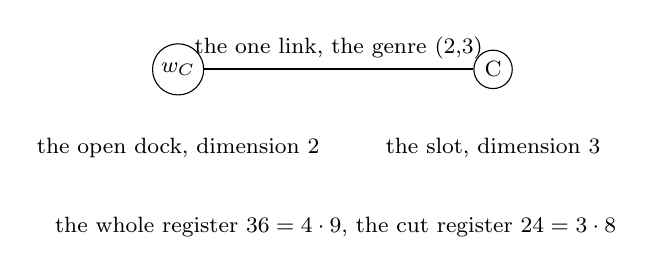
\begin{tikzpicture}[every node/.style={font=\footnotesize}]
\node[circle,draw,inner sep=2pt] (a) at (0,0) {$w_C$};
\node[circle,draw,inner sep=2pt] (b) at (4,0) {C};
\draw[thick] (a) -- node[above] {the one link, the genre (2,3)} (b);
\node at (0,-1) {the open dock, dimension 2}; \node at (4,-1) {the slot, dimension 3};
\node at (2,-2) {the whole register $36=4\cdot 9$, the cut register $24=3\cdot 8$};
\end{tikzpicture}
\caption{The one link derived of the register tower. The open dock of the horizon web at dimension two and its slot at dimension three, the read genre (2,3), whose whole and cut registers give the tower twenty-four multiplied by thirty-six to the wave.}
\end{figure}
\par\medskip\noindent{\itshape Gravity read at the counting face, Part VII turns to the photon.}\label{narr:close:10-10}\par
\section{The frame as the qubit end of the two two link}\label{mod:X-11-frame-as-the-qubit-end-of-the-two-two-link}
\chdesig{6-11}{10-11}{X-11-frame-as-the-qubit-end-of-the-two-two-link}{X-11-frame-as-the-qubit-end-of-the-two-two-link}
\begin{chwall}[The frame as the qubit end of the two two link]\label{box:X-11-frame-as-the-qubit-end-of-the-two-two-link:1}
Face A, every frame and Lorentz open result an instance of the Lorentz theorem at a qubit end of a (2,2) link, reads no. Face B reads yes with the first open result named: the Lorentz theorem carries one exact object at every one of the 510 qubit ends of the 255 (2,2) links of the 64 settled webs, the 486 sites of fifty-five webs, the Gram with the unit entry 4 and every direction entry $-1$ at the signature one against three, the isometry algebra of dimension 6 with the rotation stabiliser of dimension 3, the fifteen brackets equal to the theorem at each end with two further generators closing to minus a rotation, the frame orbit the orbit of the stabiliser on the three directions, 8 frames under the 32 monomials of the matching group at the determinant one with the kernel of the lift the 4 phases and the full rotation minus one, the pair ket the unit at 2 of 2 ends fixed by 32 monomials and 32 pairs and the transport identity at 3 of 3, exact at 510 of 510 ends; but of the eleven frame and Lorentz open results only one parts at such an end, the own-site sign at the tau port, re-met as an instance, the full rotation at that port the square of the half rotation equal to minus one equal to the swap sign, and the ten part elsewhere, three at the hub F of the first web at dimension 4, one at its qutrit core, one at the (4,4) Higgs word, one at a hub-forming move, one at a text open result and three at a qubit end of a (2,3) link beside, 4 of 11 at any qubit end; the first open result whose parting is not at a qubit end is the frame-words open result at the item order, a site-less parting at a step open result, the qudit-as-the-frame-orbit open result at the order over the located sites and the unit-from-the-single-pair open result at the address order.
\end{chwall}
\chstanding{open result}
\chdeps{Definitions 1.1 to 1.6, Theorem 53.1, Theorem 54.1 and Theorems 235.1 to 235.4 and Open result 235.5}{no theorem beyond it at this release}
The object of the Lorentz theorem is re-derived at every qubit end of every (2,2) link of the sixty-four settled webs and found exact, the eleven frame and Lorentz open results are transcribed at their parting cells and typed by the site of their parting, and each parting at such an end is re-met as an instance while each parting elsewhere is named with its dimension. The frame of reference is the qubit end of the (2,2) link wherever such an end stands, and the open results part where none does. The Lorentz group, the rotation group and the holonomy stand at their own chapters.
\begin{chbridge}
In special relativity a frame of reference at a point is an orthonormal tetrad on which the Lorentz group acts, the light cone at that point is fixed by the Minkowski form, and a rotation by a full turn acts as minus one on a spinor \cite{Minkowski1908,Wigner1939,Wald1984}. The correspondence is by name.
\end{chbridge}
\begin{chproof}[finite computation with its census and its exact part]
\textit{The premises.} The axiom and the six definitions of Section~\ref{mod:FRAMEWORK}, definitions. The Lorentz group and the signature of Section~\ref{mod:III-3-lorentz-group-and-the-signature}, a theorem, and the rotation group of Section~\ref{mod:III-2-rotation-group}, a theorem. The Lorentz group at the (2,2) pair of the chapter titled The (2,2) genre, the pair ket, the serial link and the increment (chapter~\ref{mod:X-0-D540399-the-two-two-census-at-every-placement}, among the instruments), a theorem. The holonomy and the transport of records of Section~\ref{mod:XIII-6-holonomy-and-the-record-transport}, theorems and open results. The chain from the axiom to this result is five chapters deep.

\textit{The procedure.} The 255 (2,2) links of the settled webs carry 510 ends at 486 sites, every one of dimension 2, listed one per line with the web, the ket or bra, the degree, the genres and the typing, spatial at the 14 dock-link ends and internal at the 496 others. At every end the split of the unit and the three direction steps is placed, the two-by-two directions tensor the identity at the other end, the plain-trace Gram taken and its isometry algebra formed, the six generators tested inside it with their fifteen brackets against the Lorentz theorem, the frame orbit formed as the orbit of the rotation stabilizer on the three directions at the finite face under the 32 monomial matrices of the matching group, and the pair ket tested as the unit under the pair action. The eleven open results are transcribed at their parting cells from the settled copies and the site of each parting is located and typed; an open result at a qubit end of a (2,2) link is an instance if the object the theorem carries there is defined and re-met against the frame object the open result defines, and an open result at no such end is named with the dimension at its parting.

\textit{The totals.} At every one of the 510 ends the Gram reads
\begin{equation}
\begin{pmatrix} 4 & 0 & 0 & 0 \\ 0 & -1 & 0 & 0 \\ 0 & 0 & -1 & 0 \\ 0 & 0 & 0 & -1 \end{pmatrix},
\end{equation}
the imaginary parts zero at 16 of 16, the signature one against three, the algebra of dimension 6 with the stabilizer 3, the six generators isometries at 6 of 6 with the fifteen brackets equal at 15 of 15 at each end, the frame orbit 8 frames, the signed permutations at the determinant one, the kernel of the lift the 4 phases, the half rotation about the third direction squaring to the full rotation minus one, the pair ket $(1, 0, 0, 1)$ the unit at 2 of 2 ends fixed by 32 monomials and 32 pairs with the projection to the end 32 and the center 4, annihilated by the rotations at 3 of 3 and carried by the further generators at 3 of 3, the transport at 3 of 3; exact at 510 of 510 ends with the Gram equal to the theorem at 510 of 510, the smallest instance the first end of the first web worked as the Gram above. Of the eleven open results, the own-site sign at the spatial ends parts at the tau port w1 of dimension 2 at degree 1 paired to the leaf b3 at a (2,2) link, the one parting at such an end, re-met as an instance: the full rotation at w1, the square of the half rotation, equals minus one equals the swap sign $-1$, the instance yes, the parting of that open result itself, the phase $+1$ at a read opening the port at neither orientation, carried beside and re-decided never. The ten others part elsewhere: three at the hub F of the first web, dimension 4 at degree 4 with three (2,4) links and one (3,4) and no (2,2) link, the qudit-as-the-frame-orbit, the chain-orbit-modulo-junctions and the open-set-at-the-read open results; one at the qutrit core Q of that web at dimension 3, the dimension-as-the-valence open result; one at the (4,4) Higgs word, the unit-from-the-single-pair open result; one at the hub-forming move adding four sites and five links, the light-cone open result; one at the frame-words open result, a text open result parting at a step open result with no site; and three at a qubit end of a (2,3) link, the dock of the ladder web, the two dock ends of the docked one-link body and the derived directions of the one-link model, where the (2,3) end carries the Gram with the unit entry 6 and the direction entries $-3/2$ printed beside. So the instances number 1 of 11, the named 10 of 11, and face B reads yes at three orders with the first open result the frame-words open result at the item order. The gauge half from the holonomy entry re-meets at the (2,2) cell, the 32 pairs, the projection 32, the center 4 and the swap at the odd loops at the determinant $-1$, and the orientation half from the involutions entry re-meets, the end swap fixing the pair ket and the transposed frame at the determinant $-1$ the other orientation.

\textit{The check.} A qutrit end in place of the qubit end moves the Gram unit entry to 9, a struck direction moves the algebra dimension to 3, a product ket in place of the pair ket moves the unit to 0 of 2 ends, the text struck excludes the run, and the gluon word with no qubit moves the ends to 0, 5 of 5 as pinned. The controls read the same at 15 of 16, the one that differs the orientation of one genre string, twelve link labels of the table written in the reversed order which the theorem counts at the sorted pair, mis-posed at the pinned engines and typed at the return, so the control letter reads fails at the pinned grammar beside, disclosed and deciding no grade. The result was reproduced by an independent route, two engines of different construction agreeing at every cell at both runs.
\chcert{510}
\end{chproof}
\begin{figure}[h]
\centering
\begin{adjustbox}{max width=\linewidth}\begin{tabular}{lrrrr}
\hline
the Gram at the qubit end & unit & first & second & third \\
\hline
unit & 4 & 0 & 0 & 0 \\
first & 0 & $-1$ & 0 & 0 \\
second & 0 & 0 & $-1$ & 0 \\
third & 0 & 0 & 0 & $-1$ \\
\hline
\end{tabular}\end{adjustbox}
\caption{The smallest instance, the first end of the first web: the Gram of the qubit end with the signature one against three and the imaginary parts zero at 16 of 16, equal at 510 of 510 ends.}
\end{figure}
